\documentclass[oneside]{article} 
\usepackage[utf8]{inputenc}
\usepackage[T5]{fontenc} 
\usepackage[fontsize=13pt]{scrextend} 
\usepackage[paperheight=29.7cm,paperwidth=21cm,right=2cm,left=3.5cm,top=3cm,bottom=3.5cm]{geometry}
\usepackage{mathptmx} 
\usepackage{graphicx} 
\usepackage{amssymb}
\usepackage{amsmath}
\usepackage{float} 
\usepackage{tikz} 
\usetikzlibrary{calc} 
\usepackage{indentfirst} 
\renewcommand{\baselinestretch}{1.2} 
\setlength{\parskip}{6pt} 
\setlength{\parindent}{1cm} 
\usepackage{titlesec} 
\setcounter{secnumdepth}{4} 
\titlespacing*{\section}{0pt}{0pt}{10pt} 
\titleformat*{\section}{\fontsize{13pt}{0pt}\selectfont \bfseries \centering}
\titlelabel{\thetitle.\quad}
\titlespacing*{\subsection}{0pt}{6pt}{0pt} 
\titleformat*{\subsection}{\fontsize{13pt}{0pt}\selectfont \bfseries}
\titlespacing*{\subsubsection}{0pt}{0pt}{0pt} 
\titleformat*{\subsubsection}{\fontsize{13pt}{0pt}\selectfont \bfseries}
\titlespacing*{\paragraph}{0pt}{0pt}{0pt} 
\titleformat*{\paragraph}{\fontsize{13pt}{0pt}\selectfont \itshape}
\renewcommand{\figurename}{\fontsize{13pt}{0pt}\selectfont \itshape Hình}
\renewcommand{\thefigure}{\thesection.\arabic{figure}.}
\usepackage{caption}
\captionsetup[figure]{labelsep=space}
\renewcommand{\tablename}{\fontsize{13pt}{0pt}\selectfont \itshape Bảng}
\renewcommand{\thetable}{\arabic{table}.}
\captionsetup[table]{labelsep=space}
\usepackage{tabularx}
\newcolumntype{s}{>{\hsize=.1\hsize}X}
\newcolumntype{y}{>{\hsize=.2\hsize}X}
\newcolumntype{d}{>{\hsize=.1\hsize}X}
\newcolumntype{a}{>{\hsize=1.1\hsize}X}
\newcolumntype{g}{>{\hsize=5\hsize}X}
\renewcommand{\tabularxcolumn}[1]{>{\small}m{#1}}
\renewcommand{\theequation}{\thesection.\arabic{equation}} % Thay đổi đánh số phương trình mặc định
\newtheorem{theorem}{Định lý}[section]
\newtheorem{defn}[theorem]{Định nghĩa}
\newtheorem{corollary}[theorem]{Hệ quả}
\newtheorem{lemma}[theorem]{Bổ đề}
\usepackage{lipsum}
\renewcommand{\contentsname}{MỤC LỤC}
\renewcommand{\listfigurename}{DANH MỤC HÌNH VẼ}
\renewcommand{\listtablename}{DANH MỤC BẢNG BIỂU}
\renewcommand{\refname}{TÀI LIỆU THAM KHẢO}
\usepackage[unicode]{hyperref}
\usepackage{colortbl}
\definecolor{LightCyan}{rgb}{0.88,1,1}
\usepackage{forloop}
\newcounter{loopcntr}
\newcommand{\rpt}[2][1]{\forloop{loopcntr}{0}{\value{loopcntr}<#1}{#2}}
\usepackage{enumitem} 
\setitemize{itemsep=0pt,leftmargin=1.25cm,topsep = 3pt} 
\usepackage{chngcntr}
\begin{document}
\begin{titlepage}
\begin{tikzpicture}[overlay,remember picture]
\draw [line width=3pt]
    ($ (current page.north west) + (3.0cm,-2.0cm) $)
    rectangle
    ($ (current page.south east) + (-2.0cm,2.5cm) $);
\draw [line width=0.5pt]
    ($ (current page.north west) + (3.1cm,-2.1cm) $)
    rectangle
    ($ (current page.south east) + (-2.1cm,2.6cm) $); 
\end{tikzpicture}
\begin{center}
	\vspace{-12pt}  ĐẠI HỌC QUỐC GIA HÀ NỘI \\
	\textbf{\fontsize{16pt}{0pt}\selectfont TRƯỜNG ĐẠI HỌC KHOA HỌC TỰ NHIÊN}
	\vspace{0.5cm}
	\\
	\textbf{- - - - - - - - - - - - - -}
	\\
	\vspace{1.5cm}
	\textbf{NGUYỄN THỊ DIỆU LINH}
	\\
	\vspace{4cm}
	\textbf{\fontsize{19pt}{0pt}\selectfont PHÂN TÍCH VÀ MÔ PHỎNG MỘT SỐ BÀI TOÁN THỰC TẾ BẰNG PHƯƠNG TRÌNH VI PHÂN TUYẾN TÍNH SỬ DỤNG EXCEL}
	\\
	\vspace{4cm}
	LUẬN VĂN THẠC SĨ KHOA HỌC
	\vspace{1.5cm}
\end{center}
	\vspace{3cm}
	\begin{center}
		\fontsize{14pt}{0pt}\selectfont Hà Nội, 2023
	\end{center}
\end{titlepage}
\cleardoublepage
\thispagestyle{empty}
\begin{tikzpicture}[overlay,remember picture]
\draw [line width=3pt]
    ($ (current page.north west) + (3.0cm,-2.0cm) $)
    rectangle
    ($ (current page.south east) + (-2.0cm,2.5cm) $);
\draw [line width=0.5pt]
    ($ (current page.north west) + (3.1cm,-2.1cm) $)
    rectangle
    ($ (current page.south east) + (-2.1cm,2.6cm) $); 
\end{tikzpicture}
\begin{center}
\vspace{-12pt}  ĐẠI HỌC QUỐC GIA HÀ NỘI \\
\textbf{\fontsize{16pt}{0pt}\selectfont TRƯỜNG ĐẠI HỌC KHOA HỌC TỰ NHIÊN}
\vspace{0.5cm}
\\
\textbf{- - - - - - - - - - - - - -}
\\
\vspace{1.5cm}
\textbf{NGUYỄN THỊ DIỆU LINH}
\\
\vspace{4cm}
\textbf{\fontsize{19pt}{0pt}\selectfont PHÂN TÍCH VÀ MÔ PHỎNG MỘT SỐ BÀI TOÁN THỰC TẾ BẰNG PHƯƠNG TRÌNH VI PHÂN TUYẾN TÍNH SỬ DỤNG EXCEL}
\end{center}
\vspace{0.6cm}
\indexspace Chuyên ngành: Phương pháp toán sơ cấp
\vspace{-0.6cm}
\indexspace Mã số: \qquad \quad\! 60460113\\
\vspace{0.5cm}
\begin{center}
LUẬN VĂN THẠC SĨ KHOA HỌC
\vspace{1.5cm}
\\NGƯỜI HƯỚNG DẪN KHOA HỌC: TS. Hà Phi
\end{center}
\vspace{2.2cm}
\begin{center}
 \fontsize{14pt}{0pt}\selectfont Hà Nội, 2023
\end{center}
\cleardoublepage 
\pagenumbering{arabic} 
\begin{center}
	\textbf{\fontsize{15pt}{0pt}\selectfont LỜI CẢM ƠN}
\end{center}

Bản luận văn với đề tài “Phân tích và mô phỏng một số bài toán thực tế bằng phương trình vi phân tuyến tính sử dụng Excel” được thực hiện dưới sự hướng dẫn tận tình của tiến sỹ Hà Phi. Em xin bày tỏ lòng biết ơn sâu sắc tới  thầy Hà Phi, người đã dành nhiều thời gian tận tình hướng dẫn, chỉ bảo, kiểm tra, giúp đỡ em để em hoàn thành bản luận văn này.

     Em cũng xin gửi lời cảm ơn chân thành nhất tới phòng sau đại học và các thầy cô trong  khoa Toán-Cơ-Tin trường ĐH Khoa học tự nhiên-Đại học Quốc Gia Hà Nội đã tạo điều kiện tốt nhất trong quá trình em học tập cũng như bảo vệ luận văn tốt nghiệp.
     
     Qua đây tôi cũng xin cảm ơn Trường THPT Ứng Hòa A, nơi tôi đang công tác đã tạo điều kiện cho tôi trong quá trình tôi công tác và đi học ,xin cảm ơn gia đình đã luôn là chỗ dựa vững chắc cho tôi để tôi hoàn thành khóa học này.
     
     Mặc dù đã có nhiều cố gắng nhưng bản luận văn khó tránh khỏi những thiếu sót. Em rất mong nhận được sự góp ý của các thầy cô để bản luận văn được hoàn thiện hơn.
     
     Em xin chân thành cảm ơn!
%\vspace{2.2cm}
\begin{flushleft}
\begin{tabular}{c@{\hspace{9.5cm}}c} 
	&  Tác giả luận văn\\
	& \\
	&\\
	&\\
	& Nguyễn Thị Diệu Linh \\ 
\end{tabular}
\end{flushleft}
%\section*{ĐÁNH GIÁ QUYỂN ĐỒ ÁN TỐT NGHIỆP\\\fontsize{14pt}{0pt}\selectfont \vspace{4pt}\textnormal{(Dùng cho giảng viên hướng dẫn)}}
%\thispagestyle{empty}
%\vspace{-16pt}
%\hspace{-1cm}Tên giảng viên đánh giá:\dotfill\\
%Họ và tên sinh viên:\dotfill MSSV:\dotfill\\
%Tên đồ án:\dotfill\\
%\rpt[1]{\noindent\vbox spread 6pt {}\null\xleaders\hbox to 2mm {\hss . \hss}\hfill \null}\\
%\textbf{Chọn các mức điểm phù hợp cho sinh viên trình bày theo các tiêu chí dưới đây:}\\
%Rất kém (1); Kém(2); Đạt(3); Giỏi(4); Xuất sắc(5)
%\begin{table}[H]
%\begin{tabularx}{\textwidth}{ 
%    | >{\centering\arraybackslash}s
%    | >{\arraybackslash}g
%    | >{\centering\arraybackslash}d
%    | >{\centering\arraybackslash}d
%    | >{\centering\arraybackslash}d
%    | >{\centering\arraybackslash}d
%    | >{\centering\arraybackslash}d|
%}
% \hline
% \rowcolor{LightCyan}
% \multicolumn{7}{|>{\hsize=\dimexpr6\hsize+11\tabcolsep+3\arrayrulewidth\relax}X|}{\bfseries\fontsize{11pt}{0pt}\selectfont Có sự kết hợp giữa lý thuyết và thực hành (20)} \\
% \hline
%1 &\fontsize{11pt}{0pt}\selectfont Nêu rõ tính cấp thiết và quan trọng của đề tài, các vấn đề và các giả thuyết (bao gồm mục đích và tính phù hợp) cũng như phạm vi ứng dụng của đồ án & 1 & 2 & 3 & 4 & 5 \\
% \hline
% 2 & \fontsize{11pt}{0pt}\selectfont Cập nhật kết quả nghiên cứu gần đây nhất (trong nước/quốc tế) & 1 & 2 & 3 & 4 & 5 \\
%  \hline
%3 & \fontsize{11pt}{0pt}\selectfont Nêu rõ và chi tiết phương pháp nghiên cứu/giải quyết vấn đề  & 1 & 2 & 3 & 4 & 5 \\
% \hline
%4 &\fontsize{11pt}{0pt}\selectfont Có kết quả mô phỏng/thực nghiệm và trình bày rõ ràng kết quả đạt được & 1 & 2 & 3 & 4 & 5 \\
% \hline
%\rowcolor{LightCyan}
%\multicolumn{7}{|>{\hsize=\dimexpr6\hsize+11\tabcolsep+4\arrayrulewidth\relax}X|}{\bfseries\fontsize{11pt}{0pt}\selectfont Có khả năng phân tích và đánh giá kết quả (15)} \\
% \hline
%5 &\fontsize{11pt}{0pt}\selectfont Kế hoạch làm việc rõ ràng bao gồm mục tiêu và phương pháp thực hiện dựa trên kết quả nghiên cứu lý thuyết một cách có hệ thống & 1 & 2 & 3 & 4 & 5 \\
% \hline
%6 & \fontsize{11pt}{0pt}\selectfont Kết quả được trình bày một cách logic và dễ hiểu, tất cả kết quả đều được phân tích và đánh giá thỏa đáng & 1 & 2 & 3 & 4 & 5 \\
% \hline
%7 & \fontsize{11pt}{0pt}\selectfont Trong phần kết luận, tác giả chỉ rõ sự khác biệt (nếu có) giữa kết quả đạt được và mục tiêu ban đầu đề ra đồng thời cung cấp lập luận để đề xuất hướng giải quyết có thể thực hiện trong tương lai  & 1 & 2 & 3 & 4 & 5 \\
% \hline
%\rowcolor{LightCyan}
%\multicolumn{7}{|>{\hsize=\dimexpr6\hsize+11\tabcolsep+4\arrayrulewidth\relax}X|}{\bfseries\fontsize{11pt}{0pt}\selectfont Kỹ năng viết quyển đồ án (10)} \\
% \hline
%8 &\fontsize{11pt}{0pt}\selectfont Đồ án trình bày đúng mẫu quy định với cấu trúc các chương logic và đẹp mắt (bảng biểu, hình ảnh rõ ràng, có tiêu đề, được đánh số thứ tự và được giải thích hay đề cập đến; căn lề thống nhất, có dấu cách sau dấu chấm, dấu phảy v.v.), có mở đầu chương và kết luận chương, có liệt kê tài liệu tham khảo và có trích dẫn đúng quy định & 1 & 2 & 3 & 4 & 5 \\
% \hline
%9 & \fontsize{11pt}{0pt}\selectfont Kỹ năng viết xuất sắc (cấu trúc câu chuẩn, văn phong khoa học, lập luận logic và có cơ sở, từ vựng sử dụng phù hợp v.v.) & 1 & 2 & 3 & 4 & 5 \\
% \hline
%\rowcolor{LightCyan}
%\multicolumn{7}{|>{\hsize=\dimexpr6\hsize+11\tabcolsep+4\arrayrulewidth\relax}X|}{\fontsize{11pt}{0pt}\selectfont \textbf{Thành tựu nghiên cứu khoa học (5)} \emph{(chọn 1 trong 3 trường hợp)}} \\
% \hline
%10a & \fontsize{11pt}{0pt}\selectfont Có bài báo khoa học được đăng hoặc chấp nhận đăng/Đạt giải SVNCKH giải 3 cấp Viện trở lên/Có giải thưởng khoa học (quốc tế hoặc trong nước) từ giải 3 trở lên/Có đăng ký bằng phát minh, sáng chế & \multicolumn{5}{>{\hsize=\dimexpr1\hsize+\tabcolsep+5\arrayrulewidth\relax}X|}{\centering 5} \\
% \hline
%10b & \fontsize{11pt}{0pt}\selectfont Được báo cáo tại hội đồng cấp Viện trong hội nghị SVNCKH nhưng không đạt giải từ giải 3 trở lên/Đạt giải khuyến khích trong các kỳ thi quốc gia và quốc tế khác về chuyên ngành (VD: TI contest) & \multicolumn{5}{>{\hsize=\dimexpr1\hsize+\tabcolsep+5\arrayrulewidth\relax}X|}{\centering 2} \\
% \hline
%10c & \fontsize{11pt}{0pt}\selectfont Không có thành tích về nghiên cứu khoa học & \multicolumn{5}{>{\hsize=\dimexpr1\hsize+\tabcolsep+5\arrayrulewidth\relax}X|}{\centering 0} \\
% \hline
%\rowcolor{LightCyan}
%\multicolumn{2}{|>{\hsize=\dimexpr5\hsize+5\tabcolsep+8\arrayrulewidth\relax}X|}{\bfseries\fontsize{11pt}{0pt}\selectfont Điểm tổng} &
%\multicolumn{5}{>{\hsize=\dimexpr1\hsize+3\tabcolsep+9\arrayrulewidth\relax}X|}{\hspace{2cm}/50} \\
% \hline
% \rowcolor{LightCyan}
%\multicolumn{2}{|>{\hsize=\dimexpr5\hsize+5\tabcolsep+8\arrayrulewidth\relax}X|}{\bfseries\fontsize{11pt}{0pt}\selectfont Điểm tổng quy đổi về thang 10} &
%\multicolumn{5}{>{\hsize=\dimexpr1\hsize+3\tabcolsep+8\arrayrulewidth\relax}X|}{} \\
% \hline
%\end{tabularx}
%\end{table}
%\newpage
%\thispagestyle{empty}
%\noindent\emph{\textbf{Nhận xét khác} (về thái độ và tinh thần làm việc của sinh viên)}\\
%\rpt[6]{\noindent\vbox spread 6pt {}\null\xleaders\hbox to 1mm {\hss . \hss}\hfill \null\newline}\\
%
%\hspace{9cm} Ngày: ... / ... / 20...
%
%\hspace{9.3cm}\textbf{Người nhận xét}
%
%\vspace{-6pt}
%\hspace{9cm}(Ký và ghi rõ họ tên)
%\cleardoublepage
%
%\section*{ĐÁNH GIÁ QUYỂN ĐỒ ÁN TỐT NGHIỆP\\\fontsize{14pt}{0pt}\selectfont \vspace{4pt}\textnormal{(Dùng cho cán bộ phản biện)}}
%\thispagestyle{empty}
%\vspace{-16pt}
%\hspace{-1cm}Giảng viên đánh giá:\dotfill\\
%Họ và tên sinh viên:\dotfill MSSV:\dotfill\\
%Tên đồ án:\dotfill\\
%\rpt[1]{\noindent\vbox spread 6pt {}\null\xleaders\hbox to 2mm {\hss . \hss}\hfill \null}\\
%\textbf{Chọn các mức điểm phù hợp cho sinh viên trình bày theo các tiêu chí dưới đây:}\\
%Rất kém (1); Kém(2); Đạt(3); Giỏi(4); Xuất sắc(5)
%\begin{table}[H]
%\begin{tabularx}{\textwidth}{ 
%    | >{\centering\arraybackslash}s
%    | >{\arraybackslash}g
%    | >{\centering\arraybackslash}d
%    | >{\centering\arraybackslash}d
%    | >{\centering\arraybackslash}d
%    | >{\centering\arraybackslash}d
%    | >{\centering\arraybackslash}d|
%}
% \hline
% \rowcolor{LightCyan}
% \multicolumn{7}{|>{\hsize=\dimexpr6\hsize+11\tabcolsep+3\arrayrulewidth\relax}X|}{\bfseries\fontsize{11pt}{0pt}\selectfont Có sự kết hợp giữa lý thuyết và thực hành (20)} \\
% \hline
%1 &\fontsize{11pt}{0pt}\selectfont Nêu rõ tính cấp thiết và quan trọng của đề tài, các vấn đề và các giả thuyết (bao gồm mục đích và tính phù hợp) cũng như phạm vi ứng dụng của đồ án & 1 & 2 & 3 & 4 & 5 \\
% \hline
% 2 & \fontsize{11pt}{0pt}\selectfont Cập nhật kết quả nghiên cứu gần đây nhất (trong nước/quốc tế) & 1 & 2 & 3 & 4 & 5 \\
%  \hline
%3 & \fontsize{11pt}{0pt}\selectfont Nêu rõ và chi tiết phương pháp nghiên cứu/giải quyết vấn đề  & 1 & 2 & 3 & 4 & 5 \\
% \hline
%4 &\fontsize{11pt}{0pt}\selectfont Có kết quả mô phỏng/thực nghiệm và trình bày rõ ràng kết quả đạt được & 1 & 2 & 3 & 4 & 5 \\
% \hline
%\rowcolor{LightCyan}
%\multicolumn{7}{|>{\hsize=\dimexpr6\hsize+11\tabcolsep+4\arrayrulewidth\relax}X|}{\bfseries\fontsize{11pt}{0pt}\selectfont Có khả năng phân tích và đánh giá kết quả (15)} \\
% \hline
%5 &\fontsize{11pt}{0pt}\selectfont Kế hoạch làm việc rõ ràng bao gồm mục tiêu và phương pháp thực hiện dựa trên kết quả nghiên cứu lý thuyết một cách có hệ thống & 1 & 2 & 3 & 4 & 5 \\
% \hline
%6 & \fontsize{11pt}{0pt}\selectfont Kết quả được trình bày một cách logic và dễ hiểu, tất cả kết quả đều được phân tích và đánh giá thỏa đáng & 1 & 2 & 3 & 4 & 5 \\
% \hline
%7 & \fontsize{11pt}{0pt}\selectfont Trong phần kết luận, tác giả chỉ rõ sự khác biệt (nếu có) giữa kết quả đạt được và mục tiêu ban đầu đề ra đồng thời cung cấp lập luận để đề xuất hướng giải quyết có thể thực hiện trong tương lai  & 1 & 2 & 3 & 4 & 5 \\
% \hline
%\rowcolor{LightCyan}
%\multicolumn{7}{|>{\hsize=\dimexpr6\hsize+11\tabcolsep+4\arrayrulewidth\relax}X|}{\bfseries\fontsize{11pt}{0pt}\selectfont Kỹ năng viết quyển đồ án (10)} \\
% \hline
%8 &\fontsize{11pt}{0pt}\selectfont Đồ án trình bày đúng mẫu quy định với cấu trúc các chương logic và đẹp mắt (bảng biểu, hình ảnh rõ ràng, có tiêu đề, được đánh số thứ tự và được giải thích hay đề cập đến; căn lề thống nhất, có dấu cách sau dấu chấm, dấu phảy v.v.), có mở đầu chương và kết luận chương, có liệt kê tài liệu tham khảo và có trích dẫn đúng quy định & 1 & 2 & 3 & 4 & 5 \\
% \hline
%9 & \fontsize{11pt}{0pt}\selectfont Kỹ năng viết xuất sắc (cấu trúc câu chuẩn, văn phong khoa học, lập luận logic và có cơ sở, từ vựng sử dụng phù hợp v.v.) & 1 & 2 & 3 & 4 & 5 \\
% \hline
%\rowcolor{LightCyan}
%\multicolumn{7}{|>{\hsize=\dimexpr6\hsize+11\tabcolsep+4\arrayrulewidth\relax}X|}{\fontsize{11pt}{0pt}\selectfont \textbf{Thành tựu nghiên cứu khoa học (5)} \emph{(chọn 1 trong 3 trường hợp)}} \\
% \hline
%10a & \fontsize{11pt}{0pt}\selectfont Có bài báo khoa học được đăng hoặc chấp nhận đăng/Đạt giải SVNCKH giải 3 cấp Viện trở lên/Có giải thưởng khoa học (quốc tế hoặc trong nước) từ giải 3 trở lên/Có đăng ký bằng phát minh, sáng chế & \multicolumn{5}{>{\hsize=\dimexpr1\hsize+\tabcolsep+5\arrayrulewidth\relax}X|}{\centering 5} \\
% \hline
%10b & \fontsize{11pt}{0pt}\selectfont Được báo cáo tại hội đồng cấp Viện trong hội nghị SVNCKH nhưng không đạt giải từ giải 3 trở lên/Đạt giải khuyến khích trong các kỳ thi quốc gia và quốc tế khác về chuyên ngành (VD: TI contest) & \multicolumn{5}{>{\hsize=\dimexpr1\hsize+\tabcolsep+5\arrayrulewidth\relax}X|}{\centering 2} \\
% \hline
%10c & \fontsize{11pt}{0pt}\selectfont Không có thành tích về nghiên cứu khoa học & \multicolumn{5}{>{\hsize=\dimexpr1\hsize+\tabcolsep+5\arrayrulewidth\relax}X|}{\centering 0} \\
% \hline
%\rowcolor{LightCyan}
%\multicolumn{2}{|>{\hsize=\dimexpr5\hsize+5\tabcolsep+8\arrayrulewidth\relax}X|}{\bfseries\fontsize{11pt}{0pt}\selectfont Điểm tổng} &
%\multicolumn{5}{>{\hsize=\dimexpr1\hsize+3\tabcolsep+9\arrayrulewidth\relax}X|}{\hspace{2cm}/50} \\
% \hline
% \rowcolor{LightCyan}
%\multicolumn{2}{|>{\hsize=\dimexpr5\hsize+5\tabcolsep+8\arrayrulewidth\relax}X|}{\bfseries\fontsize{11pt}{0pt}\selectfont Điểm tổng quy đổi về thang 10} &
%\multicolumn{5}{>{\hsize=\dimexpr1\hsize+3\tabcolsep+8\arrayrulewidth\relax}X|}{} \\
% \hline
%\end{tabularx}
%\end{table}
%\newpage
%\thispagestyle{empty}
%\noindent\emph{\textbf{Nhận xét khác của cán bộ phản biện}}\\
%\rpt[6]{\noindent\vbox spread 6pt {}\null\xleaders\hbox to 1mm {\hss . \hss}\hfill \null\newline}\\
%
%\hspace{9cm} Ngày: ... / ... / 20...
%
%\hspace{9.3cm}\textbf{Người nhận xét}
%
%\vspace{-6pt}
%\hspace{9cm}(Ký và ghi rõ họ tên)
\cleardoublepage
 
\addtocontents{toc}{\protect\thispagestyle{empty}}
\tableofcontents 
\thispagestyle{empty}
\cleardoublepage
{\let\oldnumberline\numberline
\renewcommand{\numberline}{Hình~\oldnumberline}
\listoffigures} 
\newpage
{\let\oldnumberline\numberline
\renewcommand{\numberline}{Bảng~\oldnumberline}
\listoftables}
\newpage
\section*{MỞ ĐẦU}
\phantomsection\addcontentsline{toc}{section}{\numberline{}MỞ ĐẦU}
\noindent \textbf{Lý do chọn đề tài}

Rất nhiều bài toán trong sinh học, khoa học kỹ thuật và công nghiệp gắn liền với việc giải một phương trình vi phân, tức là một phương trình thể hiện mối liên hệ của một hàm số chưa biết (cần tìm) với các đạo hàm của nó, xem \cite{ref1}, \cite{ref4}, \cite{ref6}. Các phương trình vi phân có thể được sử dụng như một mô hình toán học để nghiên cứu về sự sinh trưởng và phát triển của một quần thể động vật, về sự phát triển của vi khuẩn, về sự phân rã chất phóng xạ, về việc làm nóng/mát các vật thể, về hỗn hợp dung dịch, về vận tốc của một vật thể rơi trong không khí, về các mạch điện, ... Phương trình vi phân là một bộ phận vô cùng quan trọng của cả toán học cơ bản (toán lý thuyết) và toán học ứng dụng (toán ứng dụng/toán công nghiệp, v.v. ). 

Trong chương trình toán Trung học phổ thông hiện nay các ứng dụng thực tiễn của toán học đã và đang được đặc biệt quan tâm. Trong thực tế các phương trình sai phân đã được đưa vào trong chương trình, tuy nhiên phạm vi ứng dụng của các phương trình sai phân trong toán học ứng dụng hẹp hơn nhiều so với các phương trình vi phân. Lí do là vì đa phần các phương trình sai phân là hệ quả của việc rời rạc hóa các phương trình vi phân. Vì vậy phần đông học sinh ít thấy được ứng dụng thực tiễn của chúng. 

Một lí do khác là cho đến nay có rất ít các tài liệu hướng dẫn về mô phỏng một bài toán thực tế sử dụng phương trình vi phân cho học sinh trung học phổ thông, xem \cite{ref3}. Theo nhiều người quan niệm phương trình vi phân hiện đang được dạy ở đại học và không nên giới thiệu cho học sinh phổ thông. Mặc dù vậy, như thể hiện trong luận văn này, các phương trình vi phân được giới thiệu ở đây đều ở mức rất cơ bản, và học sinh không cần phải giỏi, vẫn có thể hiểu và thực hành được. Bên cạnh đó, việc tìm hiểu các mô hình toán học và thực hành sử dụng Excel như một công cụ mô phỏng cũng có tác dụng giúp học sinh thấy được vai trò của toán học ứng dụng và máy tính trong việc nghiên cứu một bài toán thực tiễn, xem \cite{ref5}. Phần mềm Excel được sử dụng là phù hợp với học sinh phổ thông, giúp các em có thể thực hành được ở trường và ở nhà, dưới sự hướng dẫn của thầy cô. 

Vì những lí do trên, trong luận văn này tôi tập trung vào việc phân tích và mô phỏng một số bài toán thực tế bằng phương trình vi phân sử dụng Excel. Vì có rất nhiều lớp phương trình vi phân khác nhau (tuyến tính, phi tuyến, thuần nhất, không thuần nhất, bậc nhất hoặc bậc cao, …), và để phù hợp với học sinh trung học phổ thông nên trong luận văn này tôi chỉ lựa chọn một lớp nhỏ các phương trình vi phân tuyến tính bậc nhất và thực hiện việc mô phỏng việc giải xấp xỉ nghiệm cho bài toán giá trị ban đầu sử dụng Excel. Luận văn được thực hiện dựa trên việc tìm hiểu tài liệu chính là các cuốn sách \cite{ref3}, \cite{ref5}. Nội dung chính của luận văn được thực hiện trong phạm vi hai chương như sau.

Chương 1 của luận văn trình bày một số kiến thức chuẩn bị, bao gồm bài toán giá trị ban đầu cho phương trình vi phân tuyến tính bậc nhất, phương pháp xấp xỉ Euler tiến và cách sử dụng Excel để giải gần đúng bài toán giá trị ban~ đầu. 

Chương 2 trình bày một số mô hình toán học trong sinh học, khoa học kỹ thuật và công nghiệp sử dụng phương trình vi phân tuyến tính bậc nhất, ví dụ như các bài toán về sự sinh trưởng và phát triển của một quần thể động vật, về sự phân rã chất phóng xạ, về việc làm nóng/mát các vật thể, về hỗn hợp dung dịch, về vận tốc của một vật thể rơi trong không khí, về các mạch điện, về sự chuyển động của một vật thể trượt. Đối với mỗi mô hình này luận văn đều trình bày chi tiết về cách xây dựng mô hình, cách mô phỏng trong Excel cùng một số bài tập liên quan nhằm hướng dẫn cho học sinh tiếp thu được tốt hơn. 
\newpage
\section*{CHƯƠNG 1.  KIẾN THỨC CHUẨN BỊ}
\phantomsection\addcontentsline{toc}{section}{\numberline{}\hspace{-1cm}CHƯƠNG 1.  KIẾN THỨC CHUẨN BỊ}
\setcounter{section}{1}
\setcounter{figure}{0}
\setcounter{table}{0}
\subsection{Phương trình vi phân tuyến tính và bài toán giá trị ban đầu}
Rất nhiều bài toán trong sinh học, khoa học kỹ thuật và công nghiệp gắn liền với việc giải một phương trình vi phân, tức là một phương trình thể hện mối liên hệ của một hàm số chưa biết (cần tìm) với các đạo hàm của nó, xem \cite{ref1}, \cite{ref4}, \cite{ref6}. Luận văn này tập trung vào việc phân tích và mô phỏng (sử dụng phầm mềm Excel, xem \cite{ref2}, \cite{ref5}) các phương trình vi phân tuyến tính bậc nhất có dạng                                
\begin{equation}
	A(t)y'(t)+B(t)y=C(t),
	\label{eq:1.1}
\end{equation}
với mọi $  t \in [{t}_{0},{{t}_{f}})$       \\
trong đó $t$ là biến thời gian, $y(t)$ là hàm chưa biết, $A(t)$, $B(t)$, $C(t)$ là các hàm số nhận giá trị thực cho trước và liên tục trong khoảng    $[t_0, t_f)$        đang xét. \\
Nếu trong khoảng đang xét mà $A(t)\ne 0\,\,\forall t$ thì bằng cách chia cho $A(t)$, phương trình trên có thể đưa được về dạng         
\begin{equation}
	y'(t)+P(t)y=Q(t).
	\label{eq:1.2}
\end{equation}
Cùng với (\ref{eq:1.2}), ta cũng xét phương trình tuyến tính thuần nhất tương ứng có dạng 
\begin{equation}
	y'(t)+P(t)y=0.
	\label{eq:1.3}
\end{equation}
Các phương trình (\ref{eq:1.2}) và (\ref{eq:1.3}) đều có vô số nghiệm. Thông thường thì các phương trình đó cần được ghép cặp với một thông tin bổ sung (điều kiện ban đầu, điều kiện biên) để dẫn đến sự tồn tại duy nhất nghiệm.  Trong nhiều ứng dụng, người ta quan tâm đến bài toán giá trị ban đầu  
\begin{equation}
	\left\{ \begin{array}{l}
	y'(t)+P(t)y=Q(t) \\ 
	y({{t}_{0}})=\,{{y}_{0}} \\ 
\end{array} \right.
\label{eq:1.4}
\end{equation}
trong đó phương trình thứ hai được gọi là điều kiện ban đầu. \\
Bài toán giá trị ban đầu (\ref{eq:1.4}) có công thức nghiệm tường minh, còn được gọi là công thức biến thiên hằng số (variational of constant). Để đảm bảo cho tính toàn vẹn của luận văn, và phù hợp với học sinh phổ thông, cách xây dựng các công thức này sẽ được trình bày lại chi tiết như sau đây. \\
\underline{Bước 1:} Xét phương trình tuyến tính thuần nhất (\ref{eq:1.3}). Giả sử $y\ne 0$  khi đó phương trình  (\ref{eq:1.3}) đưa được về dạng $$\frac{y'(t)}{y(t)}  =-\,P(t).$$
Do đó lấy tích phân hai vế từ ${{t}_{0}}$ đến $t$ ta được 
\[\ln\left| y(t) \right|=-\,\,\int\limits_{{{t}_{0}}}^{t}{P(s)ds\,+\,\ln |{{C}_{1}}|\,\,\,\,\,\,\,\,\,\,\,\,\,\,\,\,\,\,({{C}_{1}}=y({{t}_{o}})\ne 0).}\]
Vì vậy ta có                           
\begin{equation}
	y(t)\,=\,\,y({{t}_{0}})\,{{e}^{-\int\limits_{{{t}_{0}}}^{t}{P(s)ds}}}\,\,\,\,\,.  
	\label{eq:1.5}
\end{equation}                                   Trong trường hợp điều kiện ban đầu chưa biết, ta có thể xét công thức nghiệm của phương trình (\ref{eq:1.3}) dưới dạng 
\begin{equation}
	y(t)\,=\,\,C\,{{e}^{-\int\limits_{{{t}_{0}}}^{t}{P(s)ds}}}.
\label{eq:1.6}
\end{equation}
\underline{Bước 2:} Trong bước này ta đi tìm nghiệm của (\ref{eq:1.2}) có dạng tương tự (\ref{eq:1.6}), tuy nhiên ở đây thay vì hằng số $C$ ta sẽ xét hàm $C(t)$. \\
Khi đó ta có
\begin{equation}
	y(t)\,=\,\,C(t)\,\,{{e}^{-\int\limits_{{{t}_{0}}}^{t}{P(s)ds}}}.
	\label{eq:1.7}
\end{equation}
Hiển nhiên $y({{t}_{0}})=C({{t}_{0}})$ và \[\frac{dy}{dt}=\dfrac{dC}{dt}\,{{e}^{-\int\limits_{_{{{t}_{0}}}}^{t}{P(s)ds}}}-P(t)\,C\,{{e}^{-\int\limits_{_{{{t}_{0}}}}^{t}{P(s)ds}}}\,.\]
Thay hệ thức này vào phương trình (\ref{eq:1.2}) ta có \[\dfrac{dC}{dt}\,{{e}^{-\int\limits_{_{{{t}_{0}}}}^{t}{P(s)ds}}}-P(t)\,C\,{{e}^{-\int\limits_{_{{{t}_{0}}}}^{t}{P(s)ds}}}\,\,+P(t)\,\,C\,{{e}^{-\int\limits_{_{{{t}_{0}}}}^{t}{P(s)ds}}}\,\,=\,\,Q(t)\,.\]
Do đó $\dfrac{dC}{dt}\,{{e}^{-\int\limits_{_{{{t}_{0}}}}^{t}{P(s)ds}}}\,=\,\,Q(t)\,$. Điều này dẫn đến \[C'(t)\,\,=\,\,{{e}^{\int\limits_{{{t}_{0}}}^{t}{P(s)ds}}}Q(t).\]
Vì $C({{t}_{0}})\,\,=\,y({{t}_{0}})\,$ nên ta có thể lấy tích phân từ ${{t}_{o}}$ đến $t$ để thu được \[C(t)\,=\,\,C({{t}_{0}})\,\,+\,\,\,\int\limits_{{{t}_{0}}}^{t}{{{e}^{\int\limits_{{{t}_{0}}}^{s}{P(z)dz}}}}\,\,Q(s)\,ds\,\,=\,\,\,\,C({{t}_{0}})\,\,+\,{{e}^{\int\limits_{{{t}_{0}}}^{t}{P(z)dz}}}\,\,\,\int\limits_{{{t}_{0}}}^{t}{{{e}^{-\int\limits_{s}^{t}{P(z)dz}}}}\,\,Q(s)\,ds\,.\]
Thay $C(t)$ vào công thức (\ref{eq:1.7}) và chú ý rằng $y({{t}_{0}})=C({{t}_{0}})$ ta thu được 
\begin{equation}
	y(t)\,=\,\,y({{t}_{0}})\,\,{{e}^{-\int\limits_{{{t}_{0}}}^{t}{P(s)ds}}}\,+\,\,\,\int\limits_{{{t}_{0}}}^{t}{{{e}^{-\int\limits_{s}^{t}{P(z)dz}}}}\,\,Q(s)\,ds.
	\label{eq:1.8}
\end{equation}
\textbf{Ví dụ 1.1.} Tìm công thức nghiệm tường minh cho bài toán giá trị ban đầu
\[\left\{ \begin{array}{l}
	 y'(t)-\dfrac{y}{t}={{t}^{2}}\,\,\,\forall \,t>\,1,\, \\ 
	 y(1)\,=\,{{y}_{0}}. \\ 
\end{array} \right.\]
\textbf{Lời giải.}\\
Áp dụng công thức (\ref{eq:1.8}) với $P\left( t \right)=-\dfrac{1}{t},\,\,Q(t)={{t}^{2}}$ ta có \[y(t)\,=\,\,y(1)\,\,{{e}^{\int\limits_{1}^{t}{\frac{1}{s}ds}}}\,+\,\,\,\int\limits_{1}^{t}{{{e}^{\int\limits_{s}^{t}{\frac{1}{z}dz}}}}\,\,{{s}^{2}}\,ds\,\,=\,\left( {{y}_{0}}-\dfrac{1}{2} \right)\,t\,+\,\dfrac{{{t}^{3}}}{2}.\]
Vậy nghiệm của phương trình là $y(t)=\dfrac{{{t}^{3}}}{2}+\left( {{y}_{0}}-\dfrac{1}{2} \right)\,t\,.$\\
\textbf{Chú ý 1.1.
} Trong một số bài toán, khi ta chưa được cho trước điều kiện ban đầu thì thay vì công thức (\ref{eq:1.8}) ta sẽ sử dụng công thức dựa trên nguyên hàm thay vì tích phân như sau
\begin{equation}
	y(t)\,=\,\,C\,{{e}^{-\int{P(t)dt}}}\,+\,{{e}^{-\int{P(t)dt}}}\,\int{{{e}^{\int{P(t)dt}}}}\,Q(t)\,dt.
\label{eq:1.9}
\end{equation}
\subsection{Giải gần đúng bài toán giá trị ban đầu bằng phương pháp Euler tiến}
Xét bài toán giá trị ban đầu (\ref{eq:1.4}), ta thấy rằng có công thức nghiệm tường minh (\ref{eq:1.8}). Tuy vậy, việc tính toán chính xác tích phân  $\int\limits_{_{{{t}_{0}}}}^{t}{P(s)ds}\,$ không phải luôn luôn thực hiện được. Mặt khác, trong nhiều bài toán ứng dụng trong thực tiễn, ta chỉ cần tính xấp xỉ nghiệm đến một mức độ chính xác nhất định. Chính vì vậy các phương pháp số được xây dựng để xấp xỉ nghiệm của bài toán (\ref{eq:1.4}). Để phù hợp với trình độ của học sinh phổ thông trung học, luận văn này chỉ xét phương pháp Euler tiến. Đây là một phương pháp cơ bản và tương đối đơn giản nhưng vẫn thường được sử dụng, xem~ \cite{ref2}.\\
Cơ sở của phương pháp Euler tiến dựa trên việc xấp xỉ đạo hàm bởi sai phân $$y'(t)\approx \dfrac{y(t+h)-y(t)}{h}.$$
trong đó $h$ là một số thực dương đủ nhỏ. Để giải bài toán giá trị ban đầu (\ref{eq:1.4}), ta chia nhỏ đoạn $\,\!\![{{t}_{0}},{{t}_{f}})$ thành N đoạn nhỏ bằng nhau, mỗi đoạn có độ dài $h$ (được gọi là bước). Đặt $\,\,\,{{t}_{n}}={{t}_{0}}+nh$, với $n=0, 1, 2, 3...$ Khi đó ta có
$$\dfrac{y({{t}_{n+1}})-y({{t}_{n}})}{h}\,\approx \,y'({{t}_{n}})=\,-P({{t}_{n}})\,y({{t}_{n}})\,+\,Q({{t}_{n}})\,\,.$$
Do đó ta có $y({{t}_{n+1}})\,\,\approx \,\,(1-hP({{t}_{n}})\,)\,y({{t}_{n}})\,\,+\,\,h\,Q({{t}_{n}})\,$.\\
Ta đặt giá trị xấp xỉ của nghiệm tại thời điểm ${{t}_{n}}$ là ${{y}_{n}}\,\approx y({{t}_{n}})$ khi đó ta có thể tính lần lượt   ${{y}_{n}}\,,\,n\,\,=\,0,\,1,2,....\,$ sử dụng công thức Euler tiến 
\begin{equation}
	{{y}_{n+1}}\,\,\approx \,\,(1-h\,P({{t}_{n}})\,)\,{{y}_{n}}\,\,+\,\,h\,Q({{t}_{n}}).
\label{eq:1.10}
\end{equation}
Trong ví dụ minh họa dưới đây, ta sẽ thấy rằng phương pháp Euler là tương đối chính xác nếu như bước $h$ là đủ nhỏ. Giá trị bước $h$ càng nhỏ thì sai số càng thấp.\\
\textbf{Ví dụ 1.2.} Xét bài toán giá trị ban đầu được đề cập trong Ví dụ 1.1.
\begin{equation}
	\left\{ \begin{array}{l}
	 y'(t)-\dfrac{y}{t}={{t}^{2}},\,\,\forall \,t>\,1,\, \\ 
	 y(1)\,\,=\,\,\dfrac{3}{2}. \\ 
\end{array} \right.
\label{eq:1.11}
\end{equation}
Theo Ví dụ 1.1. ta thấy rằng nghiệm chính xác của bài toán (\ref{eq:1.11}) là $y(t)=~\dfrac{{{t}^{3}}}{2}+~t\,.$\\
Giả sử rằng ta muốn tìm nghiệm xấp xỉ của bài toán (\ref{eq:1.11}) trên đoạn $[1,3]$, chính xác đến $4$ chữ số thập phân bằng cách sử dụng phương pháp Euler tiến. \\
Ta chia đoạn $[1,3]$ thành N đoạn nhỏ có độ dài $h$ và đặt ${{t}_{n}}:=1\,+n\,h$, ${{y}_{n}}:=y({{t}_{n}}).$ \\
Khi đó ta có thể tính lần lượt các giá trị xấp xỉ  ${{y}_{n}}\,$với $n=0,1,2,...$ sử dụng công thức
\[{{y}_{n+1}}\,\,\approx \,\,(1+\dfrac{h}{{{t}_{n}}}\,)\,{{y}_{n}}\,\,+\,\,h\,\,t_{n}^{2}.\]
Tại mỗi thời điểm ${{t}_{n}}$ ta xác định các công thức sai số như sau\\ 
Sai số tuyệt đối  tại thời điểm ${{t}_{n}}$ là  $$\Delta {{y}_{n}}:=\left| y({{t}_{n}})-{{y}_{n}} \right|\,$$ 
Sai số tương đối  tại thời điểm ${{t}_{n}}$ là \\ $$\delta {{y}_{n}}:=\dfrac{\left| y({{t}_{n}})-{{y}_{n}} \right|\,}{\left| y({{t}_{n}}) \right|}\,\,\times \,\,100\%=\dfrac{\Delta {{y}_{n}}}{\left| y({{t}_{n}}) \right|}\times \,\,100\% $$\\
Trong khi sai số tuyệt đối xác định sai số so với nghiệm chính xác thì sai số tương đối cho thấy mức độ sai số tính theo phần trăm. Sai số tương đối phù hợp hơn sai số tuyệt đối trong những bài toán mà nghiệm chính xác quá lớn hoặc quá nhỏ, xem [2,4]. Sau đây ta đi thực hiện quá trình xấp xỉ nghiệm trên trong Excel.\newpage
\noindent \underline{Bước 1:} Nhập các tham số sử dụng trong công thức $(h, n, y(1)).$
\begin{center}
	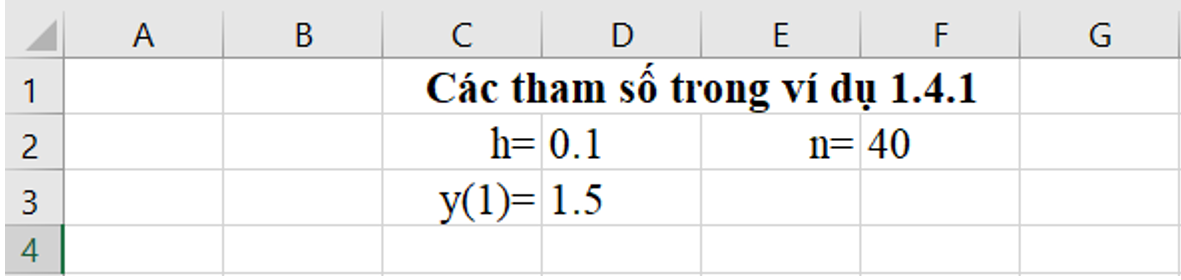
\includegraphics[scale=0.6]{Images/cac_tham_so_trong_vidu_1_4_1}
\end{center}
\underline{Bước 2:} Lập bảng gồm các cột: $n$, ${{t}_{n}}$, nghiệm xấp xỉ, nghiệm chính xác, sai số tuyệt đối, sai số tương đối (\%). \\
\underline{Bước 3.} Tính giá trị ở các cột.\\
+ Cột n: nhận các giá trị từ $0$ đến $40$.\\
+ Cột ${{t}_{n}}$ được tính bằng công thức ${{t}_{n}}:=1\,+n\,h$
\begin{center}
	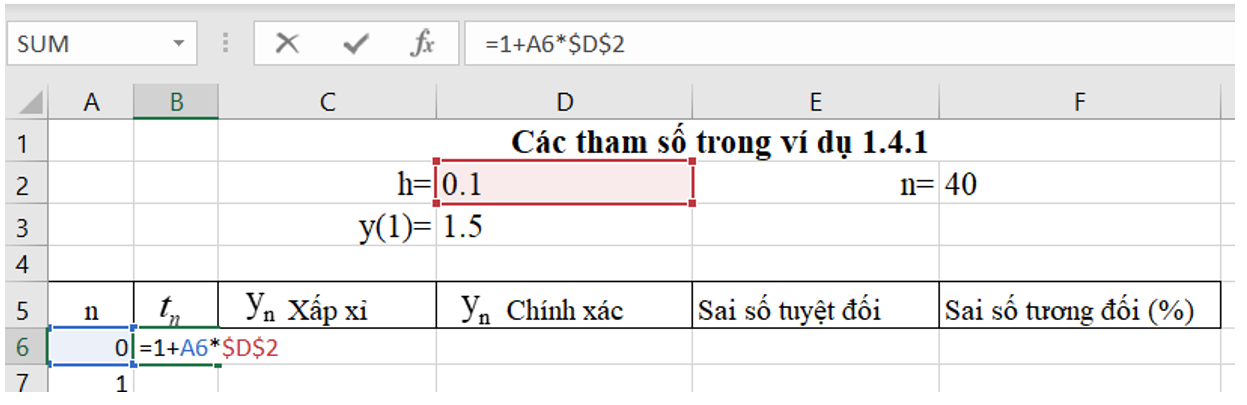
\includegraphics[scale=0.7]{Images/cac_tham_so_trong_vidu_1_4_1t}
\end{center}
+ Cột ${{y}_{n}}$ xấp xỉ được tính bằng công thức ${{y}_{n+1}}\,\,\approx \,\,(1+\dfrac{h}{{{t}_{n}}}\,)\,{{y}_{n}}\,\,+\,\,h\,\,t_{n}^{2}.$
\begin{center}
	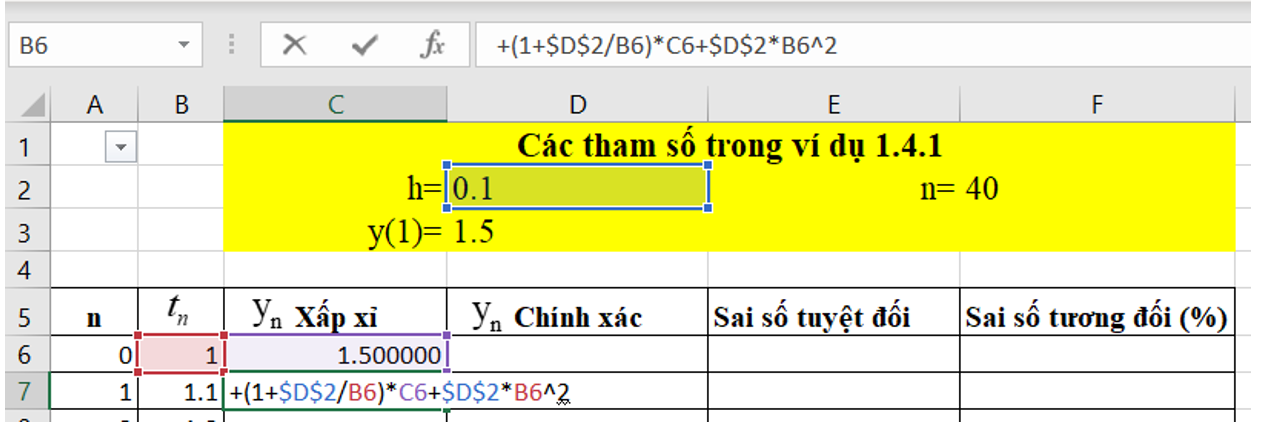
\includegraphics[scale=0.7]{Images/cac_tham_so_trong_vidu_1_4_1tt}
\end{center}\newpage
+ Cột ${{y}_{n}}$ chính xác được tính bằng công thức $y(t)=\dfrac{{{t}^{3}}}{2}+t\,.$
\begin{center}
	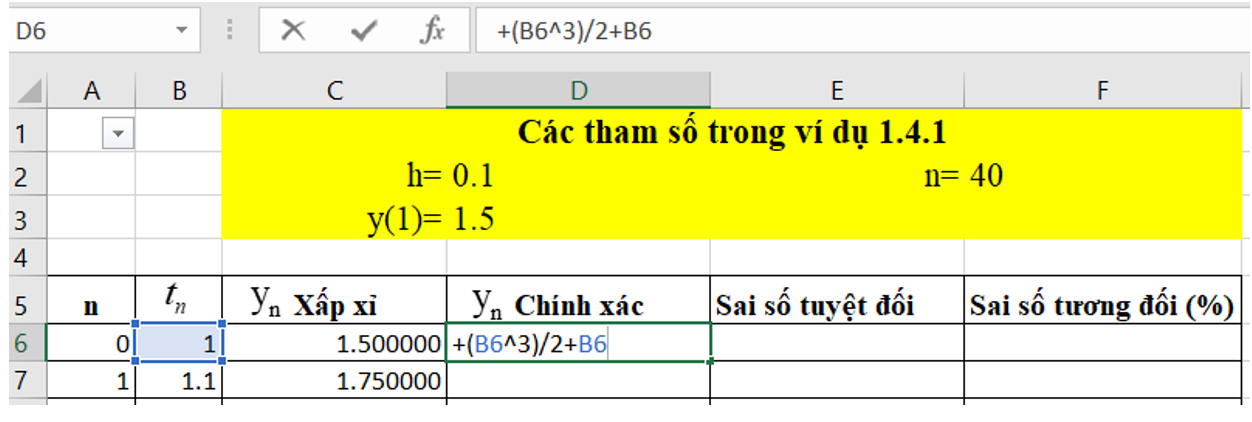
\includegraphics[scale=0.7]{Images/cac_tham_so_trong_vidu_1_4_1ttt}
\end{center}
+ Sai số tuyệt đối được tính bằng công thức  $\left|y_n\right.$ chính xác $-$ $y_n$ xấp xỉ $\left.\right|$
\begin{center}
	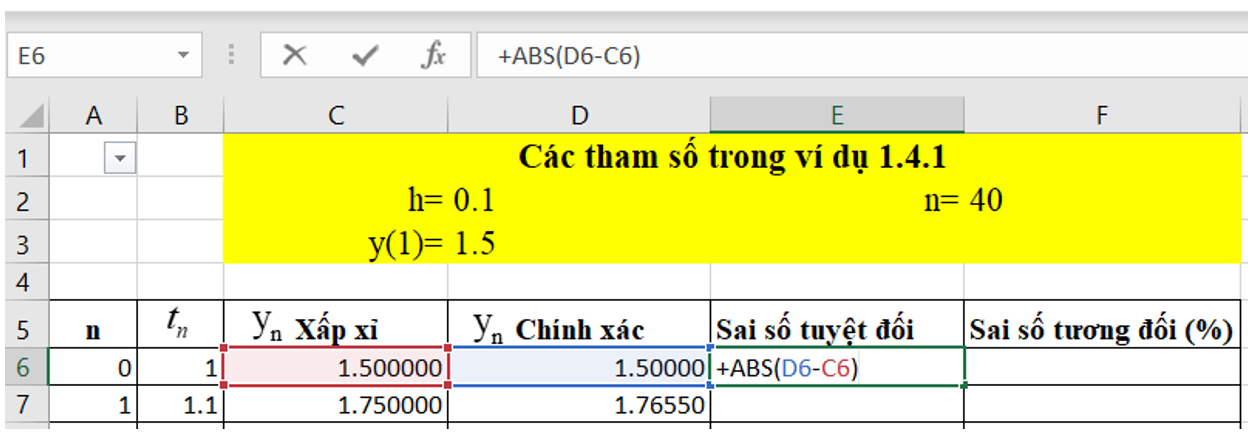
\includegraphics[scale=0.7]{Images/cac_tham_so_trong_vidu_1_4_1tttt}
\end{center}
	+ Sai số tương đối (\%) được tính bằng công thức
\begin{center}
	(Sai số tuyệt đối : ${{y}_{n}}$ chính xác) x 100
\end{center}
\begin{center}
	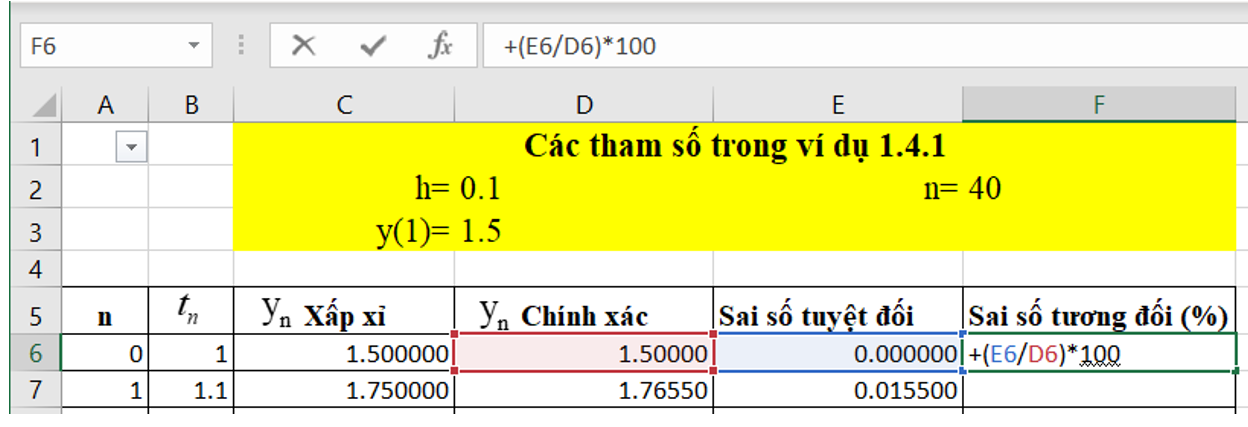
\includegraphics[scale=0.7]{Images/cac_tham_so_trong_vidu_1_4_1t5}
\end{center}
\underline{Bước 4.} Vẽ đồ thị\\
+ Ta trích xuất $1$ bảng gồm các giá trị tương ứng với số thứ tự $n$ chia hết cho $5$ (ta sử dụng filter để lọc dữ liệu) 
\begin{center}
	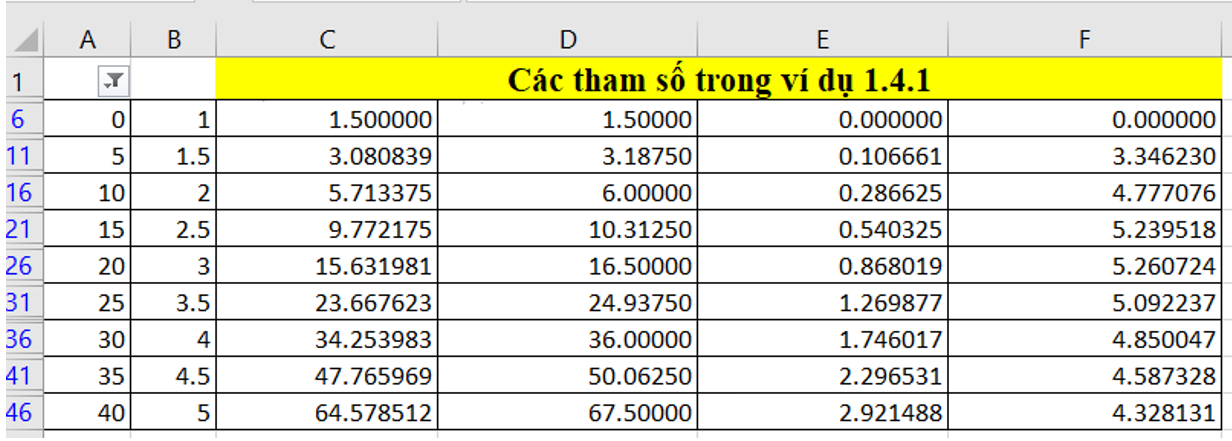
\includegraphics[scale=0.7]{Images/cac_tham_so_trong_vidu_1_4_1t6}
\end{center}
+ Từ bảng trích xuất ta vẽ đồ thị nghiệm xấp xỉ: \\
Chọn $2$ cột ${{t}_{n}}$ và nghiệm xấp xỉ $\rightarrow$  chọn insert $\rightarrow$ chọn insert line or Area chart \newline$\rightarrow$ chọn vào dạng đồ thị phù hợp
\begin{center}
	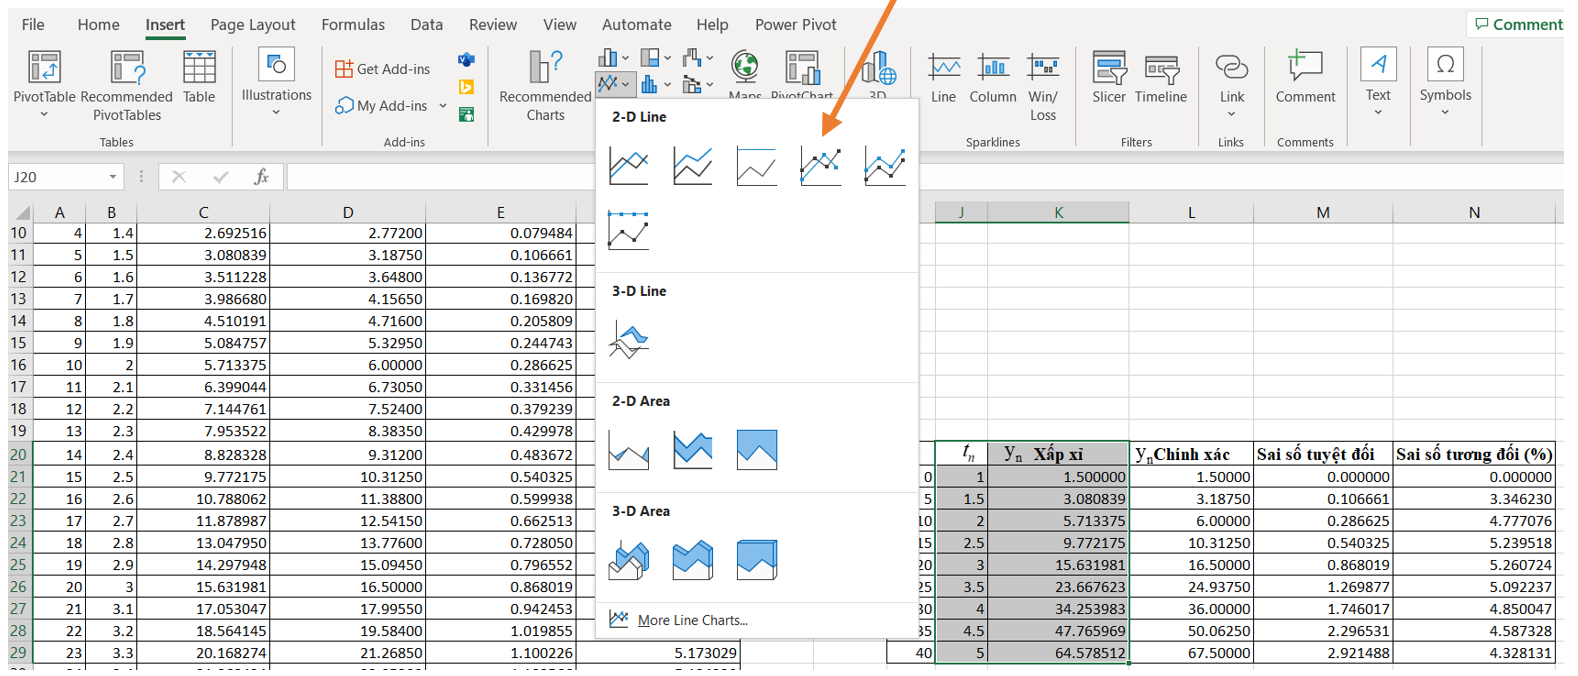
\includegraphics[scale=0.57]{Images/cac_tham_so_trong_vidu_1_4_1t7}
\end{center}
+ Để vẽ đồ thị sai số tuyệt đối và sai số tương đối của nghiệm xấp xỉ:\\
Chọn $2$ cột sai số tuyệt đối và sai số tương đối $\rightarrow$ chọn insert $\rightarrow$ chọn insert line or Area chart $\rightarrow$ chọn vào dạng đồ thị phù hợp
\begin{center}
	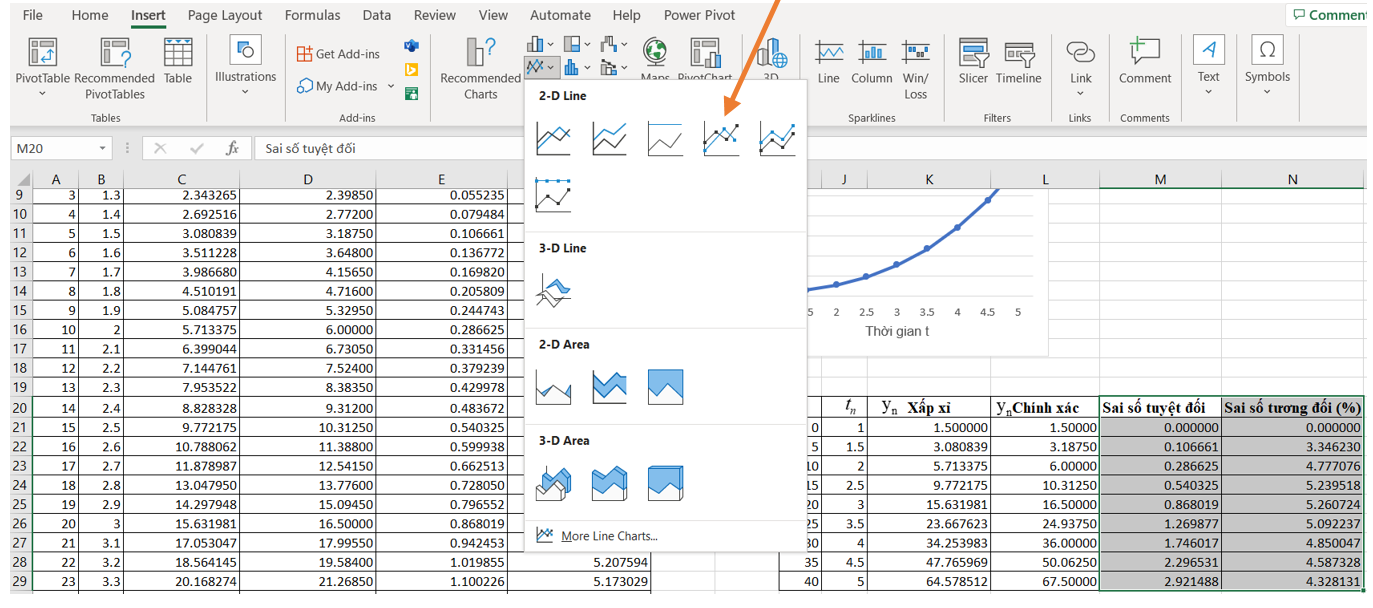
\includegraphics[scale=0.65]{Images/cac_tham_so_trong_vidu_1_4_1t8}
\end{center}
Xét trường hợp $h = 0.1$, trong bảng dưới đây ta giải số nghiệm của (\ref{eq:1.11}) cùng với sai số tuyệt đối và sai số tương đối tại mỗi giá trị ${{t}_{n}}\,$.
\begin{table}[H]
	\centering
	\begin{tabularx}{\textwidth}{
			|>{\centering\arraybackslash}s
			|>{\centering\arraybackslash}s
			|>{\centering\arraybackslash}y
			|>{\centering\arraybackslash}y
			|>{\centering\arraybackslash}y
			|>{\centering\arraybackslash}y|
		}
		\hline
		\bfseries  n  
		&\bfseries  $\mathbf{t}_{\mathbf{n}}$
		& \bfseries Nghiệm 
		xấp xỉ
		& \bfseries Nghiệm 
		chính xác
		& \bfseries Sai số 
		tuyệt đối
		& \bfseries Sai số 
		tương đối (\%)
		\\
		\hline
		0 &	1	 &   1.5000	&   1.5000  & 0.0000 &	0.0000 \\ \hline
		1 &	1.1	 &   1.7500 &  	1.7655  & 0.0155 &	0.8779 \\ \hline
		2 &	1.2	 &   2.0301 &	2.0640  & 0.0339 &	1.6429 \\ \hline
		3 &	1.3	 &   2.3433	&   2.3985  & 0.0552 &	2.3029 \\ \hline
		4 &	1.4	 &   2.6925	&   2.7720  & 0.0795 &	2.8674 \\ \hline
		5 &	1.5	 &   3.0808	&   3.1875  & 0.1067 &	3.3462 \\ \hline
		6 &	1.6	 &   3.5112	&   3.6480  & 0.1368 &	3.7492 \\ \hline
		7 &	1.7	 &   3.9867	&   4.1565  & 0.1698 &	4.0857 \\ \hline
		8 &	1.8	 &   4.5102	&   4.7160  & 0.2058 &	4.3641 \\ \hline
		9 &	1.9	 &   5.0848	&   5.3295  & 0.2447 &	4.5922 \\ \hline
		10 & 2	 &   5.7134	&   6.0000  & 0.2866 &	4.7771 \\ \hline
		11 & 2.1 &	 6.3990	&   6.7305  & 0.3315 &	4.9247 \\ \hline
		12 & 2.2 &	 7.1448	&   7.5240  & 0.3792 &	5.0404 \\ \hline
		13 & 2.3 &	 7.9535	&   8.3835  & 0.4300 &	5.1289 \\ \hline
		14 & 2.4 &	 8.8283	&   9.3120  & 0.4837 &	5.1941 \\ \hline
		15 & 2.5 &	 9.7722	&   10.3125 & 0.5403 &	5.2395 \\ \hline
		
		
	\end{tabularx}
	\caption[Bảng số liệu giá trị nghiệm bằng phương pháp Euler tiến với $h = 0.1.$]{\itshape\fontsize{13pt}{0pt}\selectfont Bảng số liệu giá trị nghiệm bằng phương pháp Euler tiến với $h = 0.1.$}
	\label{bang1}
\end{table}
\begin{figure}[H]
	\centering
	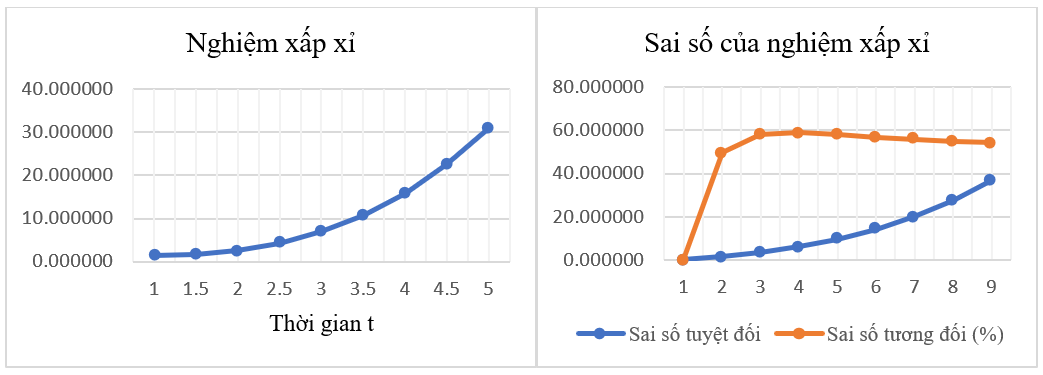
\includegraphics[scale=0.7]{Images/hinh_1_1.png}
	\caption[Biểu đồ nghiệm xấp xỉ và sai số với bước $h = 0.1.$]{\itshape\fontsize{13pt}{0pt}\selectfont Biểu đồ nghiệm xấp xỉ và sai số với bước $h = 0.1.$}
	\label{hinh1}
\end{figure}
Để minh họa tính chính xác của phương pháp Euler tiến, ta sẽ đi tìm hiểu xem sai số của nghiệm sẽ giảm như thế nào khi ta giảm bước đi một nửa. Kết quả được thể hiện trong Bảng \ref{bang2} dưới đây.
\begin{table}[H]
	\centering
	\begin{tabularx}{\textwidth}{
			|>{\centering\arraybackslash}s
			|>{\centering\arraybackslash}s
			|>{\centering\arraybackslash}y
			|>{\centering\arraybackslash}y
			|>{\centering\arraybackslash}y
			|>{\centering\arraybackslash}y|
		}
		\hline
		\bfseries  Bước h  
		&\bfseries   Số đoạn N
		& \bfseries Giá trị xấp xỉ y(t) tại t=3
		& \bfseries Giá trị chính xác y(t=3)
		& \bfseries Sai số 
		tuyệt đối
		& \bfseries Sai số 
		tương đối (\%)
		\\
		\hline
		0.4  & 5  & 13.368928 & 16.5 & 3.131072 & 18.97619149 \\ \hline
		0.2  & 10 & 14.824187 & 16.5 & 1.675813 & 10.15643952 \\ \hline
		0.1  & 20 & 15.631981 & 16.5 & 0.868019 & 5.260723841 \\ \hline
		0.05 & 40 & 16.058116 & 16.5 & 0.441884 & 2.678084966 \\ \hline
	\end{tabularx}
	\caption[Kết quả xấp xỉ tính bằng phương pháp Euler tiến với giá trị bước khác nhau.]{\itshape\fontsize{13pt}{0pt}\selectfont Kết quả xấp xỉ tính bằng phương pháp Euler tiến với giá trị bước khác nhau.}
	\label{bang2}
\end{table}
Từ Bảng \ref{bang2} ta thấy rằng khi bước $h$ giảm thì sai số của nghiệm xấp xỉ giảm. Trong ví dụ này khi bước $h$ giảm đi một nửa thì sai số dường như cũng giảm đi một nửa. Điều này phù hợp với kiến thức giảng dạy ở bậc đại học, tức là phương pháp Euler tiến có cấp chính xác là $1$, xem \cite{ref2}.\\
\textbf{Chú ý 1.2.} Có rất nhiều các phương pháp số khác nhau để giải bài toán giá trị ban đầu (\ref{eq:1.4}), và không nhất thiết phải chọn bước $h$ luôn là $1$ hằng số. Tuy nhiên để phù hợp với trình độ học sinh THPT, luận văn này được giới hạn ở phương pháp Euler tiến với bước $h$ là hằng số. Để tham khảo thêm các phương pháp khác, xem tài liệu \cite{ref2}, \cite{ref3}, \cite{ref5}.
\newpage
\section*{CHƯƠNG 2. PHÂN TÍCH VÀ MÔ PHỎNG MỘT SỐ MÔ HÌNH  THỰC TẾ SỬ DỤNG PHƯƠNG TRÌNH VI PHÂN TUYẾN TÍNH}
\phantomsection\addcontentsline{toc}{section}{\numberline{}\hspace{-1cm}CHƯƠNG 2. PHÂN TÍCH VÀ MÔ PHỎNG MỘT SỐ MÔ HÌNH  THỰC TẾ SỬ DỤNG PHƯƠNG TRÌNH VI PHÂN TUYẾN TÍNH}
\setcounter{section}{2}
\setcounter{subsection}{0}
\setcounter{figure}{0}
\setcounter{table}{2}
\setcounter{equation}{0}
Trong chương này luận văn trình bày chín mô hình toán học (sử dụng phương trình vi phân tuyến tính) được áp dụng phổ biến trong thực tiễn. Với mỗi mô hình cụ thể luận văn trình bày các bước theo thứ tự như sau.
\begin{itemize}
	\item[i)]	Xây dựng mô hình
	\item[ii)]	Trình bày một số bài tập lý thuyết để củng cố và kiểm tra lại kiến thức của học sinh.
	\item[iii)]	Thực hiện mô phỏng bằng Excel để kiểm chứng lại kết quả lý thuyết.  
\end{itemize}
Số lượng mô hình được trình bày trong luận văn là tương đối nhiều, nhằm mục đích trang bị và cung cấp một nguồn tư liệu tham khảo phong phú, tương thích với nhiều môn học trong chương trình THPT như sinh học, hóa học, cơ học, điện, khảo cổ học. Các mô hình được trình bày ở đây với mong muốn rằng một học sinh, dù không nhất thiết phải khá, giỏi trong môn toán, vẫn có thể tìm thấy một mô hình toán học thú vị và có thể tự thực hiện mô phỏng được tương đối thành thạo trong Excel. \\
Các mô hình cơ bản, phù hợp với học sinh trung bình/khá được trình bày trong các mục từ Mục 2.1 đến Mục 2.5.\\
Các mô hình còn lại (từ Mục 2.6 đến Mục 2.9) phù hợp hơn với học sinh khá/giỏi và yêu thích môn Vật lý.
\subsection{Mô hình sự tăng trưởng của vi khuẩn}
\subsubsection{Xây dựng mô hình.}
Xét một loại vi khuẩn có số lượng ban đầu tại thời điểm ${{t}_{o}}=0$ là $P_o$ và $P =~ P(t)$ là số lượng vi khuẩn tại thời điểm t. Khi đó $$P'(t):=\,\underset{\Delta t\to 0}{\mathop{\lim }}\,\dfrac{P(t+\Delta t)-P(t)}{\Delta t}=~\underset{\Delta t\to 0}{\mathop{\lim }}\,\dfrac{\Delta P}{\Delta t}.$$ thể hiện tốc độ tăng trưởng của vi khuẩn tại thời điểm t.\\
Trong thực tế, tốc độ tăng trưởng của vi khuẩn tại một thời điểm t tỷ lệ thuận với số lượng vi khuẩn P(t), do đó mô hình tăng trưởng của vi khuẩn được biểu diễn dưới dạng bài toán giá trị ban đầu                              
\begin{equation}
	\left\{\begin{array}{l}
	 P'(t)=kP, \\ 
	 P({{t}_{0}})={{P}_{0}}. \\ 
\end{array} \right.
\label{eq:2.1}
\end{equation}
trong đó $k$ là hằng số tỉ lệ. Sau đây ta xét hai trường hợp.
\begin{itemize}
	\item[i)]	Nếu $k>0$ thì ${P}'(t)>0$, khi đó $P(t)$ là hàm đồng biến chứng tỏ lượng vi khuẩn tăng dần khi thời gian $t$ tăng.
	\item[ii)]	Nếu $k<0\,$ thì ${P}'(t)<0$, khi đó $P(t)$ là hàm nghịch biến chứng tỏ lượng vi khuẩn giảm dần khi thời gian $t$ tăng.
\end{itemize}
\textbf{Ví dụ 2.1.1. } Một mẫu cấy ban đầu có số lượng vi khuẩn là ${{P}_{0}}$, tại $t = 1$ giờ số lượng vi khuẩn đo được là $\dfrac{3}{2}{{P}_{0}}$. Xác định công thức tính $P(t)$ ?\\
\textbf{Lời giải. }\\
Xét bài toán giá trị ban đầu (\ref{eq:2.1}) với thời điểm ban đầu $\,{{t}_{0}}=0$. Áp dụng công thức nghiệm (\ref{eq:1.5}) ta có $P(t)={{P}_{0}}{{e}^{kt}}$. Khi $t=1 $ theo giả thiết ta có phương trình                              
$$\dfrac{2}{3}{{P}_{0}}={{P}_{0}}{{e}^{k}}\,\Leftrightarrow \,\,{{e}^{k}}=\dfrac{2}{3}\,\,\Leftrightarrow \,\,k=ln\dfrac{2}{3}\Leftrightarrow k\approx 0.4055.$$
Vậy $P(t)={{P}_{0}}{{e}^{0.4055t}}$. 
\subsubsection{Bài tập}
\noindent\textbf{Bài 2.1.1.} Trong mô hình tăng trưởng của vi khuẩn ở Ví dụ 2.1.1, hãy xác định thời gian cần thiết để số lượng vi khuẩn tăng lên gấp ba lần?\\
\textbf{Lời giải. }\\
Theo Ví dụ 2.1.1 số lượng vi khuẩn tại thời điểm t được tính bằng công thức $$P(t)={{P}_{0}}{{e}^{0.4055t}}.$$
Khi số vi khuẩn tăng lên gấp $3$ lần nghĩa là $P(t)=3{{P}_{0}}$, ta có $3{{P}_{0}}={{P}_{0}}{{e}^{0.4055t}}$ kéo theo $0.4055t = \ln 3$ hay $t=\dfrac{\ln 3}{0.4055}\approx 2.71$ (giờ).\\
Vậy sau khoảng $2.71$ giờ số lượng vi khuẩn tăng lên gấp $3$ lần.
\begin{figure}[H]
	\centering
	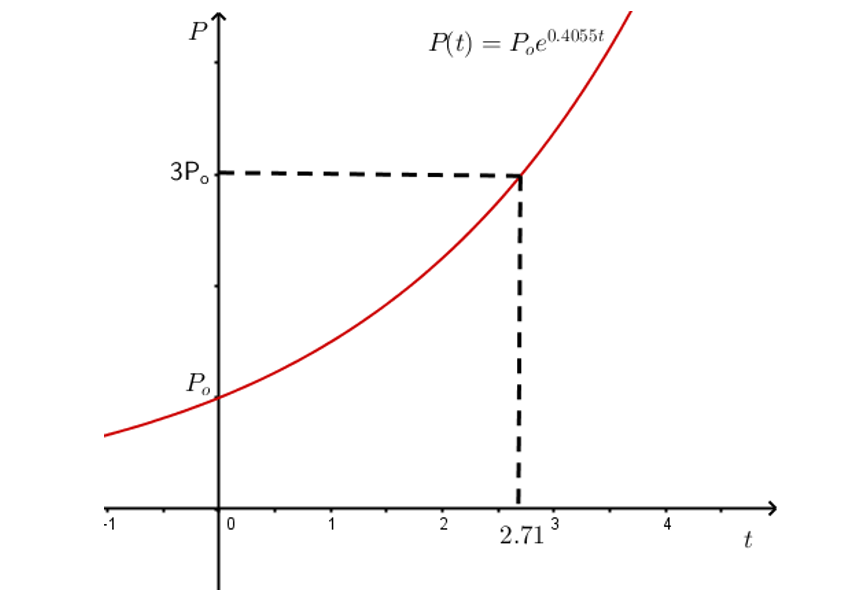
\includegraphics[scale=0.55]{Images/hinh_2_1.png}
	\caption[Thời gian mà lượng vi khuẩn tăng gấp 3 lần.]{\itshape\fontsize{13pt}{0pt}\selectfont Thời gian mà lượng vi khuẩn tăng gấp 3 lần.}
	\label{hinh2.1}
\end{figure}
\noindent\textbf{Bài 2.1.2.} Quần thể vi khuẩn trong môi trường nuôi cấy phát triển với tốc độ tỉ lệ thuận với số lượng vi khuẩn hiện có. Sau $3 $ giờ quan sát thấy có $400$ vi khuẩn. Sau $10$ giờ có $2000$ vi khuẩn. Hãy tính số lượng vi khuẩn ban đầu?\\
\textbf{Lời giải.} \\ Gọi $P=P(t)$ là số lượng vi khuẩn tại thời điểm $t$ và $P_o$ là số lượng vi khuẩn ban đầu. Từ bài toán giá trị ban đầu (\ref{eq:2.1}) và công thức (\ref{eq:1.5}) ta thu được nghiệm  $$P={{P}_{o}}{{e}^{kt}}.$$  
Theo giả thiết  $P(3) = 400$ và $P(10) = 2000$ ta có hệ phương trình
$$\left\{\begin{array}{l}
		{{P}_{0}}{{e}^{3k}}=400 \\ 
		 {{P}_{0}}{{e}^{10k}}=2000 \\ 
	\end{array}\right.
\Leftrightarrow \left\{
	\begin{array}{l}
		{{e}^{k}}={{(400/{{P}_{0}})}^{1/3}} \\ 
		{{P}_{0}}{{(400/{{P}_{0}})}^{10/3}}=2000 \\ 
	\end{array}\right.$$
Từ hệ phương trình ta có
$$	\begin{array}{l}
{{P}_{0}}^{-7/3}=\dfrac{2000}{{{400}^{10/3}}}\\ \Rightarrow {{P}_{0}}={{\left( \dfrac{2000}{{{400}^{10/3}}} \right)}^{-3/7}}\approx 201.
 	\end{array}$$
Vậy số lượng vi khuẩn ban đầu là ${{P}_{o}}\approx 201$ con.
\subsubsection{Mô phỏng bằng Excel.}
Xét mô hình tăng trưởng của vi khuẩn trong Ví dụ 2.1.1, trong đó số lượng vi khuẩn là nghiệm của bài toán giá trị ban đầu (\ref{eq:2.1}).\\ Với $k=0.4055$ và giả sử số lượng vi khuẩn ở thời điểm ban đầu t=0 là ${{P}_{0}}=100\,\,$ (con). Theo công thức nghiệm (\ref{eq:1.5}) ta có $P(t)=100{{e}^{0.4055t}}$.\\ Áp dụng công thức Euler tiến (\ref{eq:1.10}), ta có công thức nghiệm xấp xỉ \\ $${{P}_{n+1}}\approx \,(1\,\,+\,\,0.4055\,h\,)\,{{P}_{n}}.$$
Với bước $h = 0.1$ ta có bảng số liệu sau (ta chỉ trích xuất các giá trị tương ứng với các số thứ tự $n$ chia hết cho $3$).
\begin{table}[H]
	\centering
	\begin{tabularx}{\textwidth}{
			|>{\centering\arraybackslash}s
			|>{\centering\arraybackslash}s
			|>{\centering\arraybackslash}y
			|>{\centering\arraybackslash}y
			|>{\centering\arraybackslash}y
			|>{\centering\arraybackslash}y|
		}
		\hline
		\bfseries  n
		&\bfseries   $\mathbf{t}_{\mathbf{n}}$
		& \bfseries Giá trị xấp xỉ $P_n$
		& \bfseries Giá trị chính xác $P(t_n)$
		& \bfseries Sai số 
		tuyệt đối
		& \bfseries Sai số 
		tương đối (\%)
		\\
		\hline
		0  & 0     & 100.000 & 100.000 & 0.000000 & 0.000000 \\ \hline
		3  & 0.300 & 112.665 & 112.936 & 0.270917 & 0.239886 \\ \hline
		6  & 0.600 & 126.934 & 127.545 & 0.611192 & 0.479196 \\ \hline
		9  & 0.900 & 143.010 & 144.044 & 1.034141 & 0.717933 \\ \hline
		12 & 1.200 & 161.122 & 162.678 & 1.555355 & 0.956097 \\ \hline
		15 & 1.500 & 181.528 & 183.721 & 2.193062 & 1.193689 \\ \hline
		18 & 1.800 & 204.519 & 207.487 & 2.968545 & 1.430712 \\ \hline
		21 & 2.90  & 230.421 & 234.328 & 3.906629 & 1.667165 \\ \hline
		24 & 2.400 & 259.604 & 264.640 & 5.036236 & 1.903052 \\ \hline
		27 & 2.700 & 292.482 & 298.873 & 6.391028 & 2.138373 \\ \hline
		30 & 3.000 & 329.525 & 337.535 & 8.010149 & 2.373129 \\ \hline
	\end{tabularx}
	\caption[Bảng số liệu mô hình tăng trưởng vi khuẩn trong Ví dụ 2.1.1]{\itshape\fontsize{13pt}{0pt}\selectfont Bảng số liệu mô hình tăng trưởng vi khuẩn trong Ví dụ 2.1.1}
	\label{bang3}
\end{table}
\begin{figure}[!ht]
	\centering
	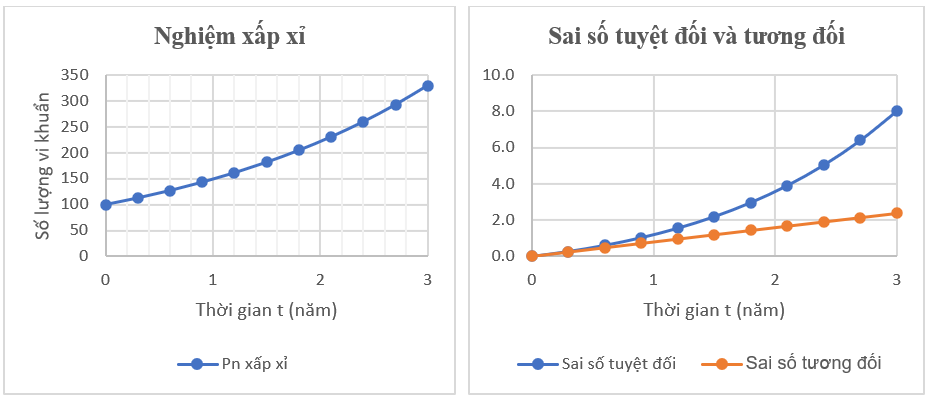
\includegraphics[scale=0.8]{Images/hinh_2_2.png}
	\caption[Biểu đồ sự tăng trưởng của vi khuẩn trong Mục 2.1.1 tính bằng phương pháp Euler tiến với bước h = 0.1.]{\itshape\fontsize{13pt}{0pt}\selectfont\centering Biểu đồ sự tăng trưởng của vi khuẩn trong Mục 2.1.1 tính bằng phương pháp Euler tiến với bước h = 0.1.}
	\label{hinh2.2}
\end{figure}
Nhìn vào Hình \ref{hinh2.2} ta thấy rằng sau khoảng $2.7$ giờ thì số lượng vi khuẩn là $300$, gấp $3$ lần số lượng vi khuẩn tại thời điểm ban đầu. Điều này rất phù hợp với kết quả tính toán lý thuyết trong Bài 2.1.1.
\subsection{Sự phân rã của đồng vị phóng xạ Plutonium-239}
\subsubsection{Xây dựng mô hình}
Hạt nhân của nguyên tử bao gồm sự kết hợp của proton và neutron. Nhiều khi sự kết hợp giữa proton và neutron này không ổn định, nghĩa là các nguyên tử phân rã hoặc biến đổi thành nguyên tử của một chất khác. Những chất chứa các hạt nhân như vậy được gọi là chất phóng xạ. Trong vật lý, chu kỳ bán rã là thước đo độ ổn định của chất phóng xạ. Chu kỳ bán rã là thời gian để một nửa số nguyên tử trong một lượng ban đầu $A_0$  phân hủy, hoặc chuyển hóa thành các nguyên tử của nguyên tố khác. Chu kỳ bán rã của chất càng dài thì chất đó càng bền. Ví dụ, chu kỳ bán rã của Ra-226 là khoảng 1700 năm. Trong 1700 năm, một nửa lượng Ra-226  được biến đổi thành radon Rn-222. Đồng vị uranium phổ biến nhất, U-238 có chu kỳ bán rã xấp xỉ 4.5 tỉ năm, trong khoảng 4.5 tỉ năm, một nửa số lượng U-238 được biến đổi thành chì, Pb-206.

Để mô hình hóa hiện tượng phân rã của chất phóng xạ, ta giả thiết rằng tốc độ phân rã $A'(t)$ tỷ lệ với số hạt nhân $A(t)$ của chất còn lại tại thời điểm $t$ với $k$ là hằng số tỷ lệ $(k <0)$, ta có phương trình $A'(t)=kA$. Nếu gọi $A_0$ là lượng chất phóng xạ ban đầu tại thời điểm $t=0$ thì lượng chất phóng xạ còn lại tại thời điểm $t$ là nghiệm của bài toán giá trị ban đầu 
\begin{equation}
	\left\{ \begin{array}{l}
	 A'(t)=kA, \\ 
	 A(0)={{A}_{0}}. \\ 
\end{array} \right.
\label{eq:2.2}
\end{equation}
\subsubsection{Bài tập}
\noindent\textbf{Bài 2.2.1.} Một lò phản ứng  chuyển đổi uranium-238 tương đối ổn định thành đồng vị plutonium-239. Sau $15$ năm, người ta xác định rằng 0.043\% lượng $A_0$ ban đầu của plutonium-239 đã bị phân hủy. Tìm chu kì bán rã của đồng vị này nếu tốc độ phân huỷ tỉ lệ với lượng nguyên tử còn lại.\\
\textbf{ Lời giải. }\\
Gọi $A(t)$ là lượng plutonium-239 còn lại tại thời điểm $t$ và  $A(t)$ là nghiệm của bài toán giá trị ban đầu (\ref{eq:2.2}). Áp dụng công thức (\ref{eq:1.5})  ta được $A(t)={{A}_{0}}{{e}^{kt}}.$\\
Nếu 0.043\% lượng $A_0$ ban đầu đã bị phân huỷ thì phần còn lại là 99.957\% $A_0$ . \\
Để xác định hằng số $k$, ta sử dụng $0.99957A_0 = A(15)$, nghĩa là $0.99957{{A}_{0}}=~{{A}_{0}}{{e}^{15k}}$, giải $k$ ta được $k\text{ }=\text{ }\dfrac{1}{15}ln\text{ }0.99957\text{ = - }0.00002867$. Do đó $A\left( t \right)\text{ = }{{A}_{0}}.{{e}^{-0.00002867t}}$.\\
    Chu kỳ bán rã là giá trị tương ứng của thời gian mà tại đó $A\left( t \right)\text{ = }\dfrac{1}{2}{{A}_{0}}$, ta có phương trình $\dfrac{1}{2}\text{ }{{A}_{0}}\text{ = }{{A}_{0}}.{{e}^{-0.00002867t}}\Leftrightarrow \dfrac{1}{2}\text{ = }{{e}^{-0.00002867t}}\Leftrightarrow t=\dfrac{\ln 2}{0.00002867}$ $\Leftrightarrow t\approx 24176.$\\
    Vậy chu kỳ bán rã của đồng vị plutonium-239 là $24176$ năm.\\
    \textbf{Bài 2.2.2.} Đồng vị phóng xạ của chì, Pb-209, bị phân hủy với tốc độ tỉ lệ thuận với lượng có mặt tại thời điểm $t$ và có chu kỳ bán rã là $3.3$ giờ. Nếu ban đầu có $1$ gam đồng vị này thì sau bao lâu  $90$\% khối lượng chì bị phân rã?\\
\textbf{    Lời giải.} \\
    Gọi $A = A(t)$ là khối lượng chì có mặt tại thời điểm $t$. Do tốc độ phân hủy tỷ lệ thuận với lượng chất phóng xạ có mặt tại thời điểm $t$ nên $A(t)$ là nghiệm của bài toán giá trị ban đầu (\ref{eq:2.2}), với $A(0)=1$. Áp dụng công thức (\ref{eq:1.5}) ta thu được nghiệm $A(t)={{e}^{kt}}$. Mặt khác chu kỳ bán rã là $3.3$ giờ nên $A(3.3)=\dfrac{1}{2}A(0)=\dfrac{1}{2}$ hay ${{e}^{3.3k}}=\dfrac{1}{2}$ hay $k=\dfrac{1}{3.3}\ln \dfrac{1}{2}.$\\
    Khi 90\% lượng chì đã bị phân rã thì còn lại $0.1$ gam, do đó $A(t) = 0.1$, ta có phương trình sau
    ${{e}^{t(\frac{1}{3.3}\ln \frac{1}{2})}}=0.1\Leftrightarrow t\,(\dfrac{1}{3.3}\ln \dfrac{1}{2})=\ln 0.1\Leftrightarrow t=3.3\dfrac{\ln 0.1}{\ln 0.5}\approx 10.96.\,\,\,$\\
    Vậy sau $10.96$ giờ thì 90\% khối lượng chì bị phân rã.\\
    \textbf{Bài 2.2.3. }Ban đầu có $100$ miligam một chất phóng xạ. Sau $6$ giờ khối lượng đã giảm $3$\%. Nếu tốc độ phân rã tỉ lệ với khối lượng chất có ở thời điểm t thì lượng chất còn 
    lại sau $24$ giờ là bao nhiêu, xác định chu kỳ bán rã của chất phóng xạ đó?\\
    \textbf{Lời giải. }\\
    Gọi $A = A (t)$ là lượng chất phóng xạ còn lại tại thời điểm $t$. Vì tốc độ phân rã tỉ lệ với khối lượng chất có ở thời điểm $t$ nên $A(t)$ là nghiệm của bài toán giá trị ban đầu 
    (\ref{eq:2.2}) với $A(0) = 100.$\\
    Áp dụng công thức (\ref{eq:1.5}) ta thu được nghiệm $A(t)=100{{e}^{kt}}$.
    Theo đề bài sau $6$ giờ khối lượng đã giảm $3$\% nghĩa là khối lượng còn lại là $97$ mg, ta có phương trình \\ $$A(6)=97\Leftrightarrow 100{{e}^{6k}}=97\Leftrightarrow {{e}^{6k}}=0.97\Leftrightarrow k=\dfrac{1}{6}\ln 0.97.$$
    Lượng chất phóng xạ còn lại sau $24$ giờ là $$A(24)=100{{e}^{\left(\frac{1}{6}\ln 0.97\right)24}}=100{{(0.97)}^{4}}\approx 88.5\,\,(mg)$$
    Chu kỳ bán rã là thời gian $T$ mà lượng chất phóng xạ còn lại một nửa, ta có  \newline
    $$\begin{array}{lll}
    A(T)=50\Leftrightarrow 100{{e}^{\left(\frac{1}{6}\ln 0.97\right)T}}=50\\ \Leftrightarrow {{(0.97)}^{\frac{1}{6}T}}=0.5\Leftrightarrow T=6{{\log }_{0.97}}0.5\approx ~136.5.\\
   \end{array}$$
    Vậy chu kỳ bán rã của chất phóng xạ là $T= 136.5$ giờ.\newpage
\noindent\textbf{Bài 2.2.4.} a) Coi bài toán có giá trị ban đầu (\ref{eq:2.2}) là mô hình cho sự phân rã của một chất phóng xạ. Chứng tỏ rằng chu kỳ bán rã $T$ của chất là $T=-\dfrac{1}{k}\ln 2$.\\
b) Chứng tỏ rằng lời giải của bài toán giá trị ban đầu trong phần a) có thể được viết là $A(t)={{A}_{0}}{{2}^{-t/T}}$ . \\
c) Nếu một chất phóng xạ có chu kỳ bán rã $T$ đã cho ở phần (a) thì sau bao lâu một lượng $A_0$ ban đầu của chất đó sẽ bị phân rã thành một lượng bằng $\dfrac{1}{8}{{A}_{0}}$?\\
\textbf{Lời giải.}\\
a) Áp dụng công thức (\ref{eq:1.5}) với $A(0)={{A}_{0}}$  ta có nghiệm của bài toán giá trị ban đầu (\ref{eq:2.2}) là $A(t)={{A}_{0}}{{e}^{kt}}$ . Gọi chu kỳ bán rã của chất phóng xạ là $T$, ta có
$$\begin{array}{lll}
A(T)={{A}_{0}}{{e}^{kT}}=\dfrac{1}{2}{{A}_{0}}\\ \Rightarrow {{e}^{kT}}=\dfrac{1}{2}\Rightarrow T=-\dfrac{1}{k}\ln 2.
\end{array}$$
b) Theo câu a) $k=-\dfrac{1}{T}\ln 2$, ta có công thức tính A(t)\\ $$A(t)={{A}_{0}}{{e}^{kt}} \Leftrightarrow A(t)={{A}_{0}}{{e}^{-\frac{1}{T}t\ln 2}}={{A}_{0}}{{2}^{-\frac{t}{T}}}.$$\\
c) Gọi $t$ là thời gian lượng $A_o$ ban đầu của chất đó sẽ bị phân rã thành $1$ lượng bằng $\dfrac{1}{8}{{A}_{0}}$, ta có $A(t)={{A}_{0}}{{e}^{kt}}=\dfrac{1}{8}{{A}_{0}}$ do đó  ${{e}^{kt}}=\dfrac{1}{8}$ hay $t=-\dfrac{1}{k}3\ln 2=3T$.\\
Vậy sau khoảng thời gian bằng $3$ lần chu kỳ bán rã thì lượng ${{A}_{0}}$ ban đầu của chất đó sẽ bị phân rã thành 1 lượng bằng $\dfrac{1}{8}{{A}_{0}}$.
\subsubsection{Mô phỏng bằng Excel.}
Xét mô hình phân rã của chất phóng xạ plutonium-239 là bài toán giá trị ban đầu (\ref{eq:2.2}). \\Ta giả sử $k  = -0.00002867$ và  ${{A}_{0}}=100\,\,(g)$, khi đó bài toán giá trị ban đầu trở thành $$\left\{ \begin{array}{l}
	 A\text{ }\!\!'\!\!\text{ (t) = - }0.00002867A, \\ 
	 A(0)=100. \\ 
\end{array} \right.$$
Công thức tính lượng chất phóng xạ còn lại tại thời điểm $t$ là $P(t)=100{{e}^{-0.00002867t}}$.\\
Tính gần đúng bằng phương pháp Euler tiến, áp dụng công thức (\ref{eq:1.10}) ta có \newline
${{A}_{n+1}}\approx (1-0.00002867h){{A}_{n}}$. \\Với bước $h = 0.1$ ta có bảng số liệu sau (ta chỉ trích xuất các giá trị tương ứng với các số thứ tự $n$ chia hết cho $3$)
\begin{table}[H]
	\centering
	\begin{tabularx}{\textwidth}{
			|>{\centering\arraybackslash}s
			|>{\centering\arraybackslash}s
			|>{\centering\arraybackslash}y
			|>{\centering\arraybackslash}y
			|>{\centering\arraybackslash}y
			|>{\centering\arraybackslash}y|
		}
		\hline
		\bfseries  n
		&\bfseries $\mathbf{t}_{\mathbf{n}}$
		& \bfseries $A_n$ xấp xỉ
		& \bfseries $A_n$ chính xác
		& \bfseries Sai số 
		tuyệt đối
		& \bfseries Sai số 
		tương đối (\%)
		\\
		\hline
		0  & 0     & 100         & 100         & 0           & 0           \\ \hline
		3  & 3000  & 91.64323409 & 91.75850553 & 0.115271447 & 0.125624809 \\ \hline
		6  & 6000  & 83.98482354 & 84.19623338 & 0.211409839 & 0.251091802 \\ \hline
		9  & 9000  & 76.96640843 & 77.25720546 & 0.290797031 & 0.376401177 \\ \hline
		12 & 12000 & 70.53450584 & 70.89005715 & 0.355551302 & 0.501553133 \\ \hline
		15 & 15000 & 64.6401023  & 65.04765701 & 0.407554707 & 0.626547866 \\ \hline
		18 & 18000 & 59.23828026 & 59.68675795 & 0.44847769  & 0.751385576 \\ \hline
		21 & 21000 & 54.28787585 & 54.7676771  & 0.479801249 & 0.876066458 \\ \hline
		24 & 24000 & 49.75116515 & 50.25400202 & 0.502836876 & 1.00059071  \\ \hline
		27 & 27000 & 45.59357673 & 46.11232123 & 0.51874449  & 1.124958529 \\ \hline
		30 & 30000 & 41.78342825 & 42.31197682 & 0.528548568 & 1.249170111 \\ \hline
	\end{tabularx}
	\caption[Bảng số liệu sự phân rã của plutonium-239 trong Bài tập 2.2.1.]{\itshape\fontsize{13pt}{0pt}\selectfont Bảng số liệu sự phân rã của plutonium-239 trong Bài tập 2.2.1.}
	\label{bang4}
\end{table}
\begin{figure}[!ht]
	\centering
	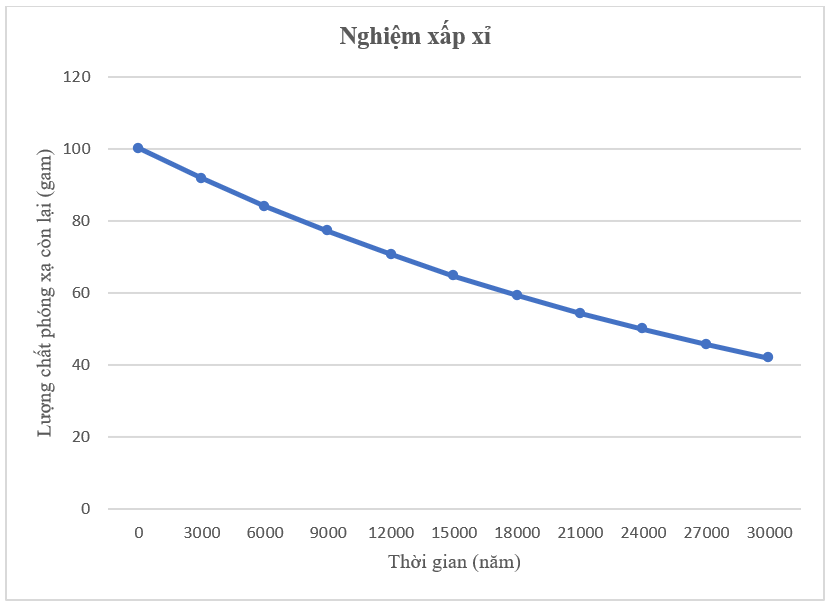
\includegraphics[scale=0.65]{Images/hinh_2_3.png}
	\caption[Biểu đồ sự phân rã của đồng vị phóng xạ plutonium-239 trong Bài tập 2.2.1. tính bằng phương pháp Euler tiến.]{\itshape\fontsize{13pt}{0pt}\selectfont\centering Biểu đồ sự phân rã của đồng vị phóng xạ plutonium-239 trong Bài tập 2.2.1. tính bằng phương pháp Euler tiến.}
	\label{hinh2.3}
\end{figure}
\noindent Nhận xét: Nhìn vào bảng số liệu và Hình \ref{hinh2.3} ta thấy sau khoảng hơn $24000$ năm khối lượng plutonium-239 giảm chỉ còn $1$ nửa. Điều này rất phù hợp với kết quả tính toán lý thuyết trong Bài 2.2.1 chu kỳ bán rã của plutonium-239 là $24176$ năm.    
\subsection{Xác định tuổi của hóa thạch}    
\subsubsection{Xây dựng mô hình xác định niên đại của carbon.}
Khoảng năm 1950, một nhóm các nhà khoa học tại Đại học Chicago do nhà hóa học Willard Libby đứng đầu đã phát minh ra một phương pháp sử dụng đồng vị phóng xạ của carbon để xác định tuổi gần đúng của vật chất hóa thạch carbon, xem \cite{ref7}. Lý thuyết xác định niên đại carbon dựa trên thực tế là đồng vị phóng xạ carbon-14 được tạo ra trong khí quyển do tác động của bức xạ vũ trụ lên nitơ-14. Tỷ lệ giữa lượng 
C-14 và C-12 bền trong khí quyển dường như là một hằng số, và kết quả là lượng tương ứng của đồng vị carbon có trong tất cả các sinh vật sống cũng giống như trong khí quyển. Khi một sinh vật sống chết đi, sự hấp thụ C-14 thông qua hô hấp, ăn uống, hoặc tổng hợp quang học chấm dứt. Bằng cách so sánh tỷ lệ tương ứng của C-14, trong một hóa thạch với tỷ lệ không đổi được tìm thấy trong khí quyển, có thể có được một ước tính hợp lý về tuổi của hóa thạch đó.

Phương pháp này dựa trên kiến    thức về chu kỳ bán rã của C-14. Giá trị tính toán của Libby về chu kỳ bán rã của C-14 là khoảng 5600 năm và được gọi là chu kỳ bán rã Libby. Ngày nay, giá trị thường được chấp nhận cho chu kỳ bán rã của C-14 là chu kỳ bán rã Cambridge gần 5730 năm. Đối với công việc của mình, Libby đã được trao giải Nobel hóa học vào năm 1960. Phương pháp của Libby đã được sử dụng để xác định niên đại cho đồ nội thất bằng gỗ được tìm thấy trong các ngôi mộ Ai Cập, các gói vải dệt của các Dead Sea Scrolls, một bản sao được phát hiện gần đây của Gnostic Gospel của Judas (Gnostic Gospels là những tác phẩm phản ánh quan điểm của những người Ngộ đạo về Cơ đốc giáo được viết trên giấy cói), và tấm vải liệm bí ẩn của thành Turin.
\begin{figure}[H]
	\centering
	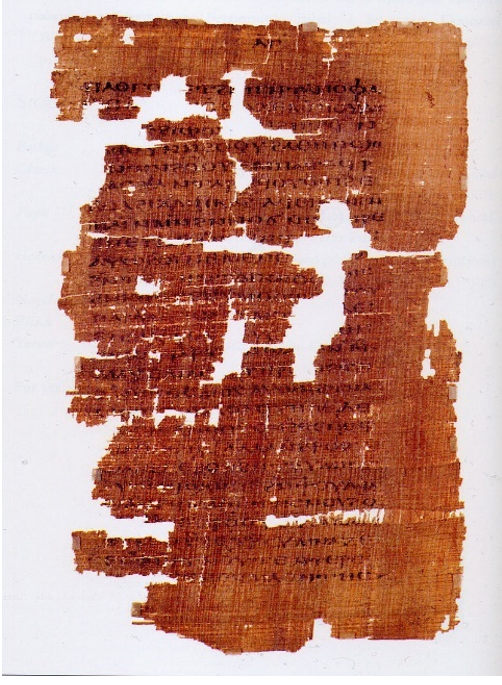
\includegraphics[scale=0.5]{Images/hinh_2_4.png}
	\caption[. Một trang trong Gnostic Gospel của Judas, xem \cite{ref4}]{\itshape\fontsize{13pt}{0pt}\selectfont\centering Một trang trong Gnostic Gospel của Judas, xem \cite{ref4}.}
	\label{hinh2.4}
\end{figure}
Gọi lượng carbon ban đầu có trong mẫu hóa thạch là $A(0)={{A}_{0}}$, và $A(t)$ là lượng carbon tại thời điểm $t$. Do tốc độ phân hủy tỷ lệ thuận với lượng carbon nên ta có phương trình vi phân (\ref{eq:2.2}) chính là bài toán giá trị ban đầu, là mô hình để xác định tuổi của hóa thạch carbon.\\
\textbf{Ví dụ 2.3.1.}  Xét mẫu xương hóa thạch được tìm thấy chứa lượng C-14 bằng 0.1\% lượng C-14 ban đầu. Hãy xác định tuổi của hóa thạch?\\
\textbf{Lời giải.  }\\
Từ bài toán giá trị ban đầu (\ref{eq:2.2}) áp dụng (\ref{eq:1.5}) ta có ngay $A(t)={{A}_{0}}{{e}^{kt}}$. \\
Để xác định giá trị của hệ số phân rã $k$, biết chu kỳ bán rã của carbon C-14 là $5730$ năm, ta sử dụng kết quả thực tế là $A(5730)=\dfrac{1}{2}{{A}_{0}}$ hay ${{A}_{0}}{{e}^{5730k}}=\dfrac{1}{2}{{A}_{0}}$.\\  
Giải phương trình
\[{{A}_{0}}{{e}^{5730k}}=\dfrac{1}{2}{{A}_{0}}\Leftrightarrow {{e}^{5730k}}=\dfrac{1}{2}\Leftrightarrow k=-\dfrac{\ln 2}{5730}\Leftrightarrow k\approx -0.00012097.\]
Do đó $A(t)={{A}_{0}}{{e}^{-0.00012097t}}.$\\
Theo giả thiết lượng carbon còn lại bằng 0.1\% lượng C-14 ban đầu nghĩa là
$$ A(t)=0.001{{A}_{0}}\Leftrightarrow {{A}_{0}}{{e}^{-0.00012097t}}=0.001{{A}_{0}} $$ 
	 $$\Leftrightarrow {{e}^{-0.00012097t}}=0.001\Leftrightarrow t=\dfrac{\ln 1000}{0.00012097}\Leftrightarrow t\approx 57103.$$
Vậy tuổi của hóa thạch là $57103$ tuổi.
\subsubsection{Bài tập}
\noindent\textbf{Bài 2.3.1.} Các nhà khảo cổ đã sử dụng những mảnh gỗ đốt, hoặc than củi, được tìm thấy tại khu vực này để xác định niên đại các bức tranh và hình vẽ thời tiền sử trên tường và trần của một hang động ở Lascaux, Pháp (xem Hình \ref{hinh2.5.}). Trong một mẩu gỗ bị đốt cháy, người ta thấy rằng  85.5\% C-14 được tìm thấy trong các cây sống cùng loại đã bị phân huỷ. Xác định tuổi của các bức tranh?
\begin{figure}[H]
	\centering
	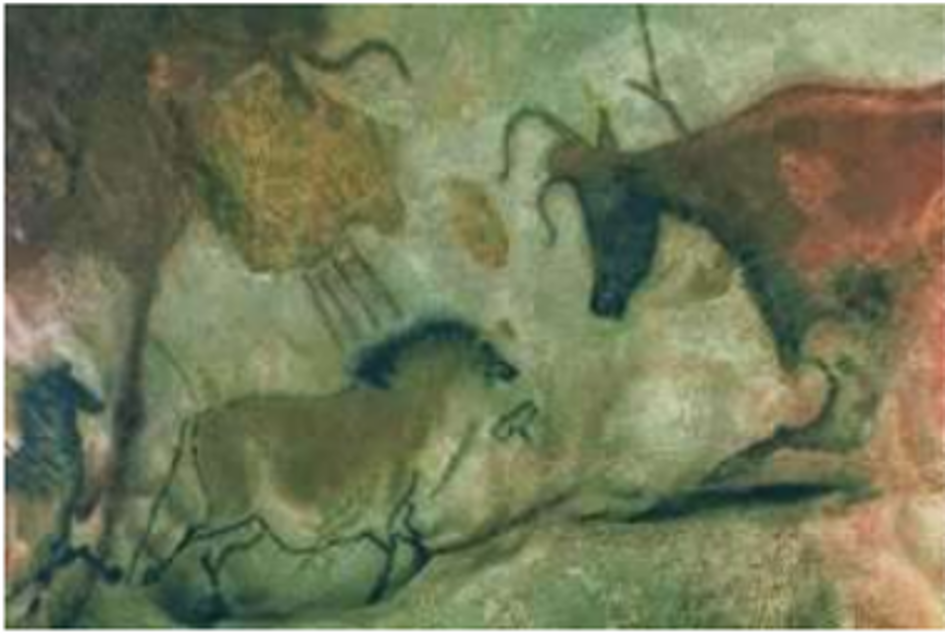
\includegraphics[scale=0.4]{Images/hinh_2_5.png}
	\caption[Bức tranh trên tường trong hang động (bức tranh đá vẽ một con ngựa và một con bò), xem \cite{ref4}.]{\itshape\fontsize{13pt}{0pt}\selectfont\centering Bức tranh trên tường trong hang động (bức tranh đá vẽ một con ngựa và một con bò), xem \cite{ref4}.}
	\label{hinh2.5.}
\end{figure}
\noindent\textbf{Lời giải}\\
Ta có chu kỳ bán rã của C-14 là $5730$ năm. Từ Mục 2.3.1 ta có công thức tính lượng carbon còn lại sau thời gian $t$ là $A(t)={{A}_{0}}{{e}^{-0.00012097t}}.$
Theo giả thiết, có 85.5\% C-14 đã bị phân hủy, nghĩa là lượng còn lại tại thời điểm $t$ là $1 -~ 0.855 =~ 0.145$ lần lượng ban đầu, nghĩa là $A(t)=0.145{{A}_{0}}$, ta có phương~ trình
$$ A(t)=0.145{{A}_{0}}\Leftrightarrow {{A}_{0}}{{e}^{-0.00012097t}}=0.145{{A}_{0}} $$
	$$\Leftrightarrow {{e}^{-0.00012097t}}=0.145\Leftrightarrow t=-\dfrac{\ln 0.145}{0.00012097}\Leftrightarrow t\approx 15963. $$
Vậy tuổi gần đúng của các bức tranh là $15963$ tuổi.\\
\textbf{Bài 2.3.2.} Tấm vải liệm thành Turin (thành phố của Ý) cho thấy hình ảnh âm bản của thi thể một người đàn ông dường như đã bị đóng đinh, được nhiều người tin rằng đó là tấm vải liệm của Chúa Giêsu thành Nazareth (xem Hình \ref{hinh2.6}). Năm $1988$, Vatican đã cho phép giám định carbon của tấm vải liệm. Ba phòng thí nghiệm độc lập của khoa học đã phân tích tấm vải và kết luận rằng tấm vải liệm đã xấp xỉ $660$ năm tuổi, độ tuổi phù hợp với hình dáng lịch sử của nó. Sử dụng độ tuổi này, hãy xác định tỷ lệ phần trăm của lượng C-14 ban đầu còn lại trong vải tính đến năm $1988$?
\begin{figure}[H]
	\centering
	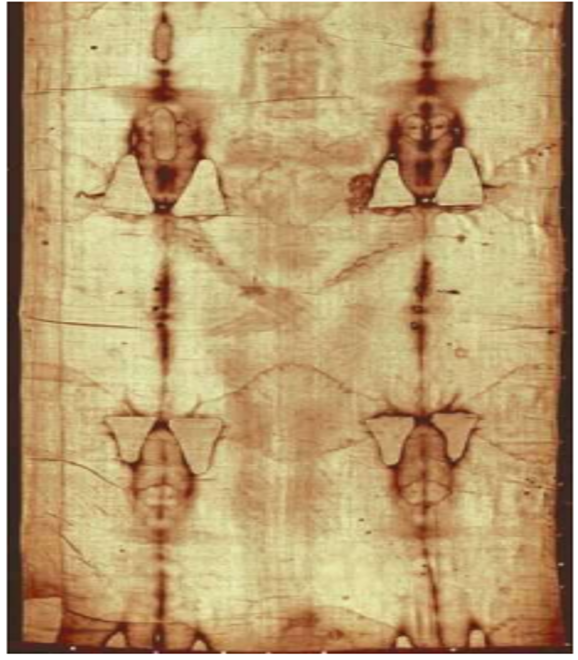
\includegraphics[scale=0.4]{Images/hinh_2_6.png}
	\caption[Tấm vải liệm thành Turin, xem \cite{ref4}.]{\itshape\fontsize{13pt}{0pt}\selectfont\centering Tấm vải liệm thành Turin, xem \cite{ref4}.}
	\label{hinh2.6}
\end{figure}
\noindent\textbf{Lời giải.}\\
Ta có chu kỳ bán rã của C-14 là $5730$ năm. Giả sử ${{t}_{0}}=0$, $A(0)={{A}_{0}}$. Từ Ví dụ 2.3.1 ta có công thức tính lượng carbon còn lại tại thời điểm $t$ là $A(t)=~{{A}_{0}}{{e}^{-0.00012097t}}$.
Theo giả thiết  $t=660$ (năm), ta có $$A(660)={{A}_{0}}{{e}^{-0.00012097\times 660}}=~{{A}_{0}}\times ~0.92326.$$
Vậy tính đến năm $1988$ lượng C-14 còn lại trong vải bằng 92.326\% so với lượng 
C-14 ban đầu.
\subsubsection{Mô phỏng bằng Excel}
Xét mẫu xương hóa thạch được tìm thấy chứa 0.1\% lượng C-14 ban đầu, với $k=-0.00012097$, bài toán giá trị ban đầu để xác định tuổi của hóa thạch là
$$\left\{ \begin{array}{l}
	 A'(t)=-0.00012097A, \\ 
	 A(0)=1000. \\ 
\end{array} \right.$$
Công thức tính số tuổi của hóa thạch là $A(t)=1000{{e}^{-0.00012097t}}$ (theo Ví dụ 2.3.1).\\
Sử dụng tính gần đúng bằng phương pháp Euler tiến với ${{t}_{n}}={{t}_{0}}+n.h$, với bước nhảy $h=200.$ Áp dụng công thức (\ref{eq:1.10}) ta có ${{A}_{n+1}}\approx (1-0.00012097h){{A}_{n}}$, ta có bảng số liệu sau (ta chỉ trích xuất bảng số liệu với giá trị của $n$ chia hết cho $5$)
\begin{table}[H]
	\centering
	\begin{tabularx}{\textwidth}{
			|>{\centering\arraybackslash}s
			|>{\centering\arraybackslash}s
			|>{\centering\arraybackslash}y
			|>{\centering\arraybackslash}y
			|>{\centering\arraybackslash}y
			|>{\centering\arraybackslash}y|
		}
		\hline
		\bfseries  n
		&\bfseries   $\mathbf{t}_{\mathbf{n}}$
		& \bfseries $A_n$ xấp xỉ
		& \bfseries $A_n$ chính xác
		& \bfseries Sai số 
		tuyệt đối
		& \bfseries Sai số 
		tương đối (\%)
		\\
		\hline
		0  & 0    & 1000        & 1000        & 0           & 0           \\ \hline
		5  & 1000 & 884.7435818 & 886.060541  & 1.31695926  & 0.148630844 \\ \hline
		10 & 2000 & 782.7712054 & 785.1032823 & 2.332076887 & 0.297040777 \\ \hline
		15 & 3000 & 692.5518    & 695.6490391 & 3.097239096 & 0.445230126 \\ \hline
		20 & 4000 & 612.7307601 & 616.3871639 & 3.656403855 & 0.593199221 \\ \hline
		25 & 5000 & 542.1096073 & 546.1563439 & 4.046736626 & 0.740948388 \\ \hline
		30 & 6000 & 479.6279957 & 483.9275856 & 4.299589912 & 0.888477954 \\ \hline
		35 & 7000 & 424.3477908 & 428.7891383 & 4.441347494 & 1.035788246 \\ \hline
		40 & 8000 & 375.4389843 & 379.9331359 & 4.494151516 & 1.182879589 \\ \hline
	\end{tabularx}
	\caption[Bảng số liệu lượng carbon C-14 còn lại sau thời gian t
	trong Ví dụ 2.3.1.]{\itshape\fontsize{13pt}{0pt}\selectfont Bảng số liệu lượng carbon C-14 còn lại sau thời gian t trong Ví dụ 2.3.1.}
	\label{bang5}
\end{table}
\begin{figure}[H]
	\centering
	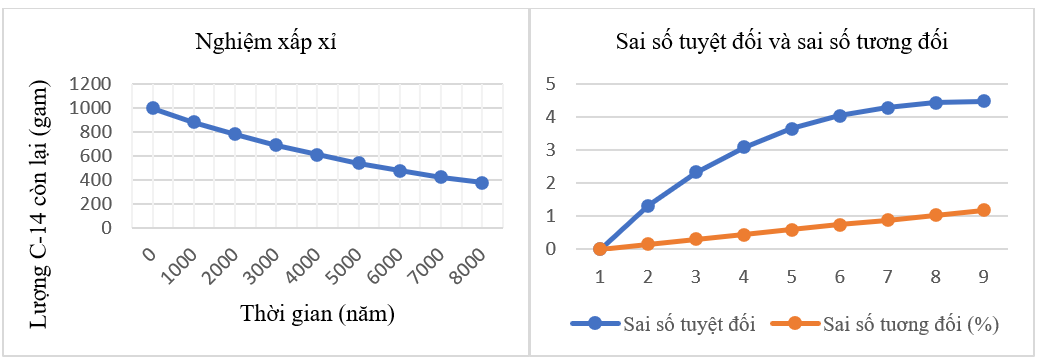
\includegraphics[scale=0.7]{Images/hinh_2_7.png}
	\caption[Biểu đồ lượng C-14 còn lại sau khoảng thời gian t và biểu đồ sai số trong Ví dụ 2.3.1 tính bằng phương pháp Euler tiến]{\itshape\fontsize{13pt}{0pt}\selectfont\centering Biểu đồ lượng C-14 còn lại sau khoảng thời gian t và biểu đồ sai số trong Ví dụ 2.3.1 tính bằng phương pháp Euler tiến}
	\label{hinh2.7}
\end{figure}
\subsection{Định luật làm mát/nóng của Newton}
\subsubsection{Xây dựng mô hình}
Theo định luật làm mát/nóng thực nghiệm của Newton, tốc độ thay đổi nhiệt độ của vật thể tỷ lệ với sự chênh lệch giữa nhiệt độ của vật thể và nhiệt độ của môi trường xung quanh, gọi là nhiệt độ môi trường. Nếu $T= T(t)$ biểu thị nhiệt độ của một vật thể tại thời điểm $t$, $T_m$ là nhiệt độ của môi trường xung quanh và ${T}'(t)$ là tốc độ thay đổi nhiệt độ của vật thể, thì định luật làm mát /nóng của Newton chuyển thành phát biểu toán học ${T}'(t)\sim \,T-{{T}_{m}}$ hay ${T}'(t)=k\left( T-{{T}_{m}} \right)$\\
Khi đó bài toán giá trị ban đầu của mô hình là 
\begin{equation}
	\left\{ \begin{array}{l}
		 {T}'(t)=k\left( T-{{T}_{m}} \right), \\ 
		 T(0)={{T}_{0}}. \\ 
	\end{array} \right.
\label{eq:2.3}
\end{equation}
với $k$ là hằng số tỉ lệ, nếu $T_m$ là một hằng số, ta xét hai trường hợp
\begin{itemize}
	\item[i)] Khi làm mát: nhiệt độ vật giảm dần khi thời gian tăng lên, chứng tỏ hàm $T(t)$ 
	nghịch biến, do đó ${T}'(t)<0 $ hay ${T}'(t)=k\left( T-{{T}_{m}} \right)<0$, mà $T>{{T}_{m}}$ nên $k<0$.
	\item[ii)] Khi làm nóng: nhiệt độ vật tăng dần khi thời gian tăng lên, chứng tỏ hàm $T(t)$ đồng biến, do đó ${T}'(t)>0$ hay ${T}'(t)=k\left( T-{{T}_{m}} \right)>0$, mà $T<{{T}_{m}}$ nên $k<0$.
\end{itemize}
Vậy trong cả hai trường hợp ta đều có hệ số $k<0.$\\
Áp dụng công thức nghiệm (\ref{eq:1.8}) cho bài toán giá trị ban đầu (\ref{eq:2.3}) ta có
\begin{equation}
	T(t)\,=\,\,\,{{T}_{0}}\,{{e}^{\int\limits_{0}^{t}{k\,ds}}}\,+\,\,\,\int\limits_{0}^{t}{{{e}^{\int\limits_{s}^{t}{k\,dz}}}}\,\,(-k\,{{T}_{m}})\,ds\,\,=\,\,{{e}^{kt}}\,({{T}_{0}}-{{T}_{m}})\,\,+\,{{T}_{m}}.
\label{eq:2.4}
\end{equation}
\textbf{Ví dụ 2.4.1.} Khi lấy một chiếc bánh ra khỏi lò, nhiệt độ của nó được đo là 150°C. Ba phút sau nhiệt độ của nó là 93°C. Hỏi phải mất bao lâu để bánh nguội đến nhiệt độ phòng là 21°C? \\
\textbf{Lời giải. }\\
Theo giả thiết nhiệt độ phòng là 21°C nên ${{T}_{m}}=21$. Khi đó bài toán giá trị ban đầu (\ref{eq:2.3}) trở thành $\left\{ \begin{array}{l}
	 {T}'(t)=k\left( T(t)-21 \right), \\ 
	 T(0)=150. \\ 
\end{array} \right.$\\
Sau khi ra lò $3$ phút thì nhiệt độ của bánh là 93°C, như vậy ta cần xác định $k$ để $T(3) = 93$. Theo công thức (\ref{eq:2.4}) ta có $T(t)\,=\,\,{{e}^{kt}}\,(150-21)\,\,+\,21\,\,$ do đó\newline $T(3)\,=\,\,{{e}^{3k}}\,(150-21)\,\,+\,21\,=93$, khi đó $k=\dfrac{1}{3}\ln \dfrac{72}{150-21}\approx -0.1944$.\\  
Vậy ta có nhiệt độ bánh tại thời điểm $t$ là $T(t)=21+129{{e}^{-0.1944t}}.$ \\
Để bánh đạt được nhiệt độ phòng thì $T(t) = 21$ hay ${{e}^{-0.1944t}}=0$, điều này là không thể xảy ra với một giá trị $t$ hữu hạn.\\ Mặc dù vậy, vì $\underset{t\to \infty }{\mathop{\lim }}\,\,\,T(t)=\,\underset{t\to \infty }{\mathop{\lim }}\,\,\,(21+129{{e}^{-0.1944t}})\,=\,21\,$ điều đó có nghĩa là sau một khoảng thời gian đủ dài thì chiếc bánh sẽ đạt xấp xỉ nhiệt độ phòng với sai số bé tùy ý. Ví dụ như để đạt đến nhiệt độ $21.15$ độ thì 
$t\approx \dfrac{-1}{0.1944}\ln \dfrac{0.15}{129}\approx 35$ (phút).
\begin{figure}[H]
	\centering
	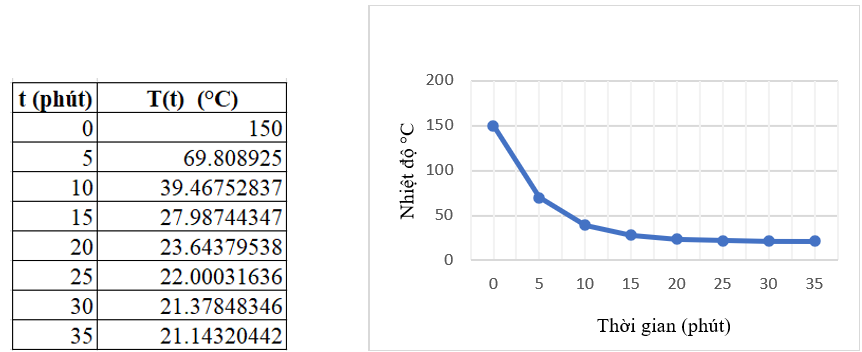
\includegraphics[scale=0.8]{Images/hinh_2_8.png}
	\caption[Biểu đồ nhiệt độ bánh được làm nguội trong Ví dụ 2.4.1.]{\itshape\fontsize{13pt}{0pt}\selectfont\centering Biểu đồ nhiệt độ bánh được làm nguội trong Ví dụ 2.4.1.}
	\label{hinh2.8}
\end{figure}
\subsubsection{Bài tập}
\noindent\textbf{Bài 2.4.1. } Một nhiệt kế được lấy ra khỏi phòng có nhiệt độ 21°C và được mang ra ngoài, nơi có nhiệt độ không khí là -12°C. Sau một nửa phút, nhiệt kế ghi 10°C. Số đo của nhiệt kế là bao nhiêu khi t =1 phút? Sau bao lâu thì nhiệt kế đạt -9°C?\\
\textbf{Lời giải. }
Ta có nhiệt độ phòng  ${{T}_{m}}=-{{12}^{o}}C$ , nhiệt độ nhiệt kế ban đầu $T(0)=21^{\circ}C$.\\
Theo định luật làm mát của Newton ta có bài toán giá trị ban đầu 
$$\left\{ \begin{array}{l}
	 {T}'(t)=k\left( T+12 \right), \\ 
	 T(0)=21. \\ 
\end{array} \right.$$
Áp dụng công thức (\ref{eq:2.4}) ta có công thức nghiệm $T(t)=-12+33{{e}^{kt}}.$\\
Mặt khác theo giả thiết ta có $T(\dfrac{1}{2})=10$ hay $ 10=-12+33\,{{e}^{\frac{k}{2}}}$, do đó $k=2\ln \dfrac{2}{3}.$\\
Nhiệt độ của nhiệt kế tại thời điểm $t$ là $T(t)=-12+33{{e}^{\left( 2\ln \frac{2}{3} \right)t}}=-12+33\,\,{{\left( \dfrac{2}{3} \right)}^{2t}}.$\\
Sau 1 phút số đo của nhiệt kế là $T(1)=-12+33(\dfrac{4}{9})={{2.67}^{o}}C.$\\
Thời gian để nhiệt độ đạt $-9^{\circ}C$ là nghiệm của phương trình  $T(t)=-12+33{{(\dfrac{2}{3})}^{2t}}=~-~9.$ do đó ${{\left( \dfrac{4}{9} \right)}^{t}}=\dfrac{1}{11}$ hay $t\approx 2.957.\,\,$ Vậy sau $2.957 $ phút nhiệt kế chỉ $-9^{\circ}C.$\\
\textbf{Bài 2.4.2.} Một nhiệt kế được đưa từ trong phòng ra bên ngoài, nơi có nhiệt độ không khí là -15°C. Sau 1 phút, nhiệt kế ghi 13°C và sau 5 phút, nhiệt kế ghi -1°C. Nhiệt độ ban đầu trong phòng là bao nhiêu?\\
\noindent\textbf{Lời giải.}
Theo định luật làm mát của Newton ta có phương trình vi phân
$$T'(t)=k(T-{{T}_{m}})=k(T+15)=kT+15k.$$
Áp dụng công thức (2.4) phương trình có nghiệm là 
$$T(t)\,=\,\,\,{{e}^{kt}}\,({{T}_{0}}-{{T}_{m}})\,\,+\,{{T}_{m}}\,\,=\,{{e}^{kt}}\,({{T}_{0}}+15)\,\,-15=C{{e}^{kt}}\,-\,15\,$$ với $C={{T}_{o}}+15$\\
Theo giả thiết $T(1)=13$, $T\left( 5 \right)=-1$, ta có hệ phương trình
$$\left\{ \begin{array}{l}
	13=C{{e}^{k}}-15 \\ 
	-1=C{{e}^{5k}}-15 \\ 
\end{array} \right.\,\,\Leftrightarrow \,\,\,\left\{ \begin{array}{l}
	 28=C{{e}^{k}} \\ 
	 14=C{{e}^{5k}} \\ 
\end{array} \right.\,\,\,\,\Leftrightarrow \,\,\,\,\left\{ \begin{array}{l}
	 28=C{{e}^{k}} \\ 
	 {{e}^{4k}}=\dfrac{1}{2} \\ 
\end{array} \right.\,\,\,\,\Leftrightarrow \,\,\,\,\left\{ \begin{array}{l}
	 k=-\dfrac{1}{4}\ln 2, \\ 
	 C\approx 33.3. \\ 
\end{array} \right.$$
Công thức tính nhiệt độ tại thời điểm $t$ là $$T(t)=-15+33.3{{e}^{(-\frac{1}{4}\ln 2)t}}=-15+33.3\times {{2}^{-\frac{t}{4}}}.$$
Nhiệt độ ban đầu trong phòng là $T(0)=-15+33.3={{18.3}^{o}}C$\\
\textbf{Bài 2.4.3.} Người ta thả một thanh kim loại nhỏ, có nhiệt độ ban đầu là 20°C vào một bình lớn đựng nước sôi. Sau bao lâu thì thanh đó đạt được 90°C nếu biết nhiệt độ của nó tăng 2°C trong 1 giây? Sau bao lâu thì thanh này đạt 98°C?\\
\textbf{Lời giải. }\\
Theo định luật làm nóng của Newton, ta có phương trình vi phân
$$T'(t)=k(T-{{T}_{m}})=k(T-100)=kT-100k.$$
Áp dụng công thức (\ref{eq:2.4}) phương trình có nghiệm 
\[T(t)\,=\,\,\,{{e}^{kt}}\,({{T}_{0}}-{{T}_{m}})\,\,+\,{{T}_{m}}\,\,=\,\,-80{{e}^{kt}}\,+100.\]
Theo giả thiết $T(1)=22$, ta có phương trình $22=-80{{e}^{k}}+100$ do đó $k=~\ln \left( \dfrac{39}{40} \right).$ \\
Công thức tính nhiệt độ thanh kim loại tại thời điểm $t$ là
$$T(t)=100-80{{e}^{t.\ln (\frac{39}{40})}}=100-80.{{(\frac{39}{40})}^{t}}.$$
Khi thanh đạt $90^{\circ}C$ nghĩa là $T(t)=100-80{{(\dfrac{39}{40})}^{t}}=90$ do đó ${{(\dfrac{39}{40})}^{t}}=\dfrac{1}{8}\,\,$\\ hay
$t={{\log }_{\frac{39}{40}}}\dfrac{1}{8}\approx 82.1.\,$ \\ \\Vậy khi $t=82.1$ giây thì thanh đạt 90°C.\\
Khi thanh đạt $98^{\circ}C$ nghĩa là $T(t)=100-80{{(\dfrac{39}{40})}^{t}}=98$ do đó ${{(\dfrac{39}{40})}^{t}}=\dfrac{1}{40}$\newline hay $t={{\log }_{\frac{39}{40}}}\frac{1}{40}\approx 145.7\,$. Vậy khi t=145.7 giây thanh đạt 98°C.\\ \\
\textbf{Bài 2.4.4.} Hai thùng lớn A và B có cùng kích thước được xếp gần nhau. Các dung dịch trong thùng chứa A và B được duy trì tương ứng ở 0°C và 100°C. Người ta hạ một thanh kim loại nhỏ có nhiệt độ ban đầu là 100°C  vào thùng A. Sau 1 phút nhiệt độ của thanh là 90°C. Sau 2 phút thanh này được lấy ra và chuyển ngay sang thùng B. Sau 1 phút ở thùng B nhiệt độ của thanh tăng lên 10°C. Sau bao lâu kể từ khi bắt đầu toàn bộ quá trình để thanh kim loại này đạt đến 99.9°C?\\
\textbf{Lời giải.}\\
Gọi ${{T}_{1}}={{T}_{1}}(t),\,\,{{T}_{2}}={{T}_{2}}(t)$ lần lượt là nhiệt độ của thanh kim loại ở thùng A và thùng B tại thời điểm $t$. Theo định luật làm mát/nóng lên của Newton, phương trình vi phân của thùng A là $\left\{ \begin{array}{l}
	 {{{{T}'}}_{1}}(t)={{k}_{1}}\left( {{T}_{1}}-0 \right)={{k}_{1}}{{T}_{1}}, \\ 
	 {{T}_{1}}(0)=100. \\ 
\end{array} \right.$\\
Áp dụng công thức (\ref{eq:2.4}) nghiệm của phương trình này là ${{T}_{1}}(t)=100{{e}^{{{k}_{1}}t}}$.  \\
Sau $1$ phút nhiệt độ của thanh kim loại là 90°C nên ta có ${{T}_{1}}(1)=100{{e}^{{{k}_{1}}}}=90$, do đó ${{e}^{{{k}_{1}}}}=0.9 $ hay $ {{k}_{1}}=\ln 0.9$. Vậy ${{T}_{1}}(t)=100{{e}^{t\ln 0.9}}.$ \\
Sau $2$ phút nhiệt độ của thanh kim loại là  ${{T}_{1}}(2)=100{{e}^{2\ln 0.9}}=100{{(0.9)}^{2}}={{81}^{o}}C.$ \\
Phương trình vi phân của thùng B là  $\left\{ \begin{array}{l} {{{{T}'}}_{2}}(t)={{k}_{2}}\left( {{T}_{2}}-100 \right)={{k}_{2}}{{T}_{2}}-100{{k}_{2}}, \\ 
	 {{T}_{2}}(0)=81. \\ 
\end{array} \right.$\\
Áp dụng công thức (\ref{eq:2.4}) nghiệm của phương trình là ${{T}_{2}}(t)=100-19{{e}^{{{k}_{2}}t}}.$\\
Sau 1 phút ở thùng B, nhiệt độ của thanh kim loại tăng lên 10°C nghĩa là đạt  ${{91}^{o}}C$, vì vậy ta có  ${{T}_{2}}(1)=100-19{{e}^{{{k}_{2}}}}=91 $ hay $ {{e}^{{{k}_{2}}}}=\dfrac{9}{19}$, do đó  ${{k}_{2}}=\ln \dfrac{9}{19}$.\\
Vậy  ${{T}_{2}}(t)=100-19{{e}^{t.\ln (9/19)}}$. \\
Khi thanh kim loại đạt 99.9°C nghĩa là $T_2(t) = 99.9$ ta có 
\[{{T}_{2}}\left( t \right)\text{ = }99.9\Leftrightarrow 100-19{{e}^{t.\ln (9/19)}}=99.9\,\Leftrightarrow {{e}^{t.\ln (9/19)}}=\dfrac{0.1}{19}\Leftrightarrow t={{\log }_{\frac{9}{19}}}\dfrac{0.1}{19}\approx 7.022\]
Do đó, từ khi bắt đầu quá trình “nhúng kép”, tổng thời gian cho đến khi thanh đạt đến 99.9°C trong thùng B là khoảng $2+7.022= 9.022$ phút.\newpage
\noindent\textbf{Bài 2.4.5. }Một nhiệt kế đọc được 21°C được đặt trong lò đã được làm nóng trước đến nhiệt độ không đổi. Qua cửa sổ kính ở cửa lò, một người quan sát ghi lại rằng nhiệt kế chỉ 43°C sau 1/2 phút và 63°C sau 1 phút. Hỏi nhiệt độ ban đầu trong lò là bao~ nhiêu?\\
\textbf{Lời giải. }\\
Gọi nhiệt độ ban đầu trong lò là   ${{T}_{m}}$. Theo định luật làm nóng của Newton ta có bài toán giá trị ban đầu là (\ref{eq:2.3}) với $T(0)=21$. \\
Áp dụng công thức (\ref{eq:2.4}) nghiệm của phương trình là \[T(t)\,=\,\,\,{{e}^{kt}}\,({{T}_{0}}-{{T}_{m}})\,\,+\,{{T}_{m}}\,\,=\,\,{{e}^{kt}}\,(21-{{T}_{m}})\,\,+\,{{T}_{m}}.\]
Theo giả thiết ta có hệ phương trình sau
\[\left\{ \begin{array}{l}
	 T(\dfrac{1}{2})=43 \\ 
	 T(1)=63 \\ 
\end{array} \right.\Leftrightarrow \left\{ \begin{array}{l}
	 (21-{{T}_{m}}){{e}^{\frac{1}{2}k}}+{{T}_{m}}=43\,\, \\ 
	 (21-{{T}_{m}}){{e}^{k}}+{{T}_{m}}=63\,\, \\ 
\end{array} \right.\Leftrightarrow \left\{ \begin{array}{l}
	 {{e}^{k/2}}=\dfrac{43-{{T}_{m}}}{21-{{T}_{m}}} \\ 
	 {{e}^{k}}=\dfrac{63-{{T}_{m}}}{21-{{T}_{m}}} \\ 
\end{array} \right.\]
Do đó ta có $\,\,\,{{({{e}^{k/2}})}^{2}}={{e}^{k}}\,\,$ hay $\,\,\,{{\left( \dfrac{43-{{T}_{m}}}{21-{{T}_{m}}} \right)}^{2}}=\dfrac{63-{{T}_{m}}}{21-{{T}_{m}}}$, giải phương trình ta được
$$
\begin{array}{ll}
 &{{(43-{{T}_{m}})}^{2}}=(63-{{T}_{m}})(21-{{T}_{m}}) \\
	 \Leftrightarrow &1849-86{{T}_{m}}+T_{m}^{2}=1323-84{{T}_{m}}+T_{m}^{2}\, \\
	\Leftrightarrow &526=2{{T}_{m}}\Leftrightarrow {{T}_{m}}=263. 
	\end{array}
	$$
Vậy nhiệt độ trong lò ban đầu là ${{263}^{o}}C.$ \\
\textbf{Bài 2.4.6. }Tại thời điểm ban đầu $t=0$, một ống nghiệm kín đựng một hoá chất được nhúng vào bể chất lỏng. Nhiệt độ ban đầu của hóa chất trong ống nghiệm là 27°C. Trong bể chất lỏng có kiểm soát nhiệt độ (đo bằng °C) được cho bởi công thức ${{T}_{m}}(t)=38-22{{e}^{-0.1t}}\,\,(t\ge 0)$, trong đó $t$ được đo bằng phút.\\
a) Giả sử rằng $k=-0.1$ trong bài toán giá trị ban đầu (\ref{eq:2.3}). Trước khi giải quyết bài 
toán, hãy mô tả bằng lời bạn mong đợi nhiệt độ $T(t)$ của hóa chất sẽ như thế nào trong một khoảng thời gian ngắn và trong khoảng thời gian dài?\\
b) Giải quyết bài toán giá trị ban đầu. Sử dụng công cụ vẽ đồ thị để vẽ biểu đồ của 
$T(t) $ và ${{T}_{m}}(t)$  trên các khoảng thời gian có độ dài khác nhau. Các đồ thị có phù hợp với dự đoán của bạn trong phần a) không?\\
\textbf{Lời giải.}\\
Nhiệt độ ban đầu của bể chất lỏng là ${{T}_{m}}(0)=38-22={{16}^{o}}C$. \\
a) Nhiệt độ ban đầu của ống nghiệm cao hơn nhiệt độ chất lỏng trong bể, nên trong thời gian ngắn ban đầu nhiệt độ hóa chất trong ống nghiệm sẽ giảm dần (nguội đi). Theo thời gian, nhiệt độ của bể sẽ tăng lên 38°C vì ${{e}^{-0.1t}}$  giảm từ $1$ về $0$ khi $t$ tăng từ $0$. Do đó, về lâu dài, nhiệt độ của hóa chất phải tăng hoặc ấm dần về  38°C.\\
b) Áp dụng định luật làm mát của Newton cho mô hình, ta có 
$${T}'(t)=k\left( T-{{T}_{m}} \right)=-0.1\left( T-38+22{{e}^{-0.1t}} \right)=-0.1T+3.8-2.2{{e}^{-0.1t}}.$$
Áp dụng công thức (1.8) cho bài toán giá trị ban đầu (\ref{eq:2.3}) trong trường hợp hàm ${{T}_{m}}(t)=38-22{{e}^{-0.1t}}\,\,(t\ge 0)$ ta có nghiệm của phương trình là
\[T(t)={{T}_{0}}{{e}^{\int\limits_{0}^{t}{k\,ds}}}+\int\limits_{0}^{t}{{{e}^{\int\limits_{s}^{t}{k\,dz}}}}(-k{{T}_{m}})ds=\,27{{e}^{\int\limits_{0}^{t}{-0.1\,ds}}}+\int\limits_{0}^{t}{{{e}^{\int\limits_{s}^{t}{-0.1\,dz}}}}(3.8-2.2{{e}^{-0.1s}})\,ds\] \[=38-(2.2t+11){{e}^{-0.1t}}.\]
Vậy $T(t)=38-(2.2t+11){{e}^{-0.1t}}$.
\begin{figure}[H]
	\centering
	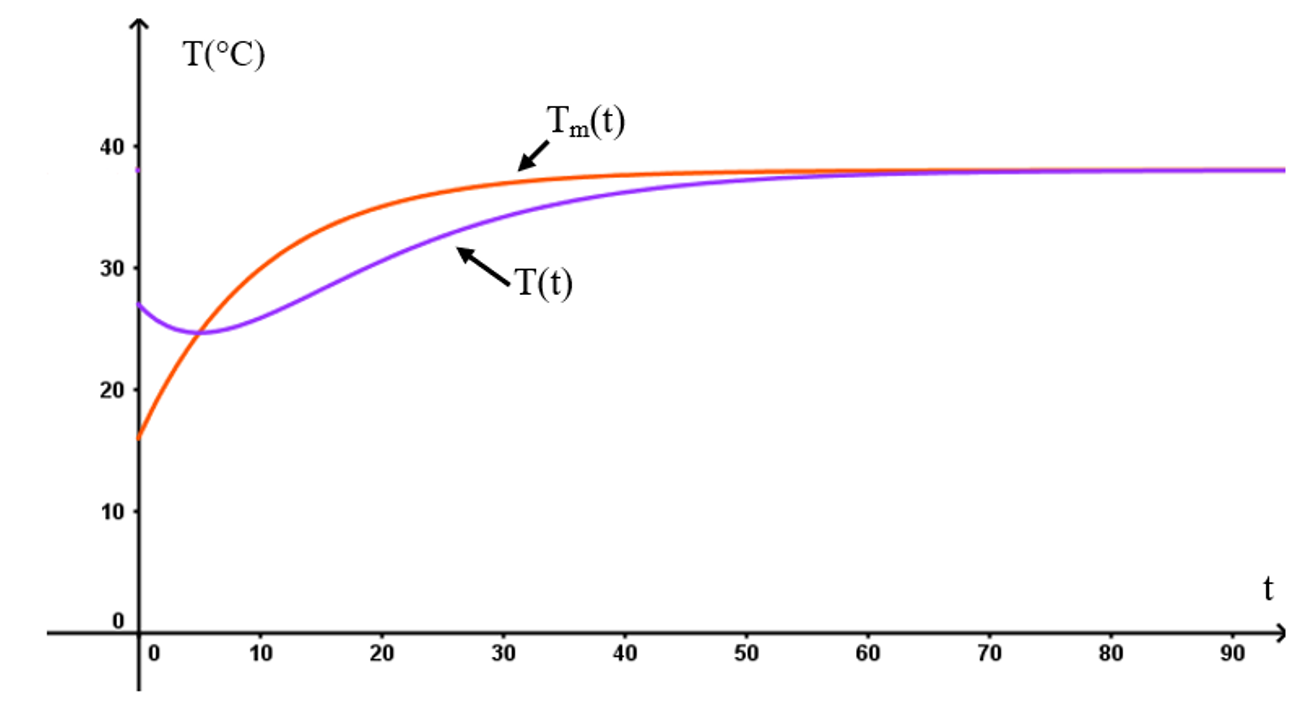
\includegraphics[scale=0.5]{Images/hinh_2_9.png}
	\caption[Đồ thị ${{T}_{m}}(t)$ và $T(t)$ trong Bài toán 2.4.6.]{\itshape\fontsize{13pt}{0pt}\selectfont\centering Đồ thị ${{T}_{m}}(t)$ và $T(t)$ trong Bài toán 2.4.6. }
	\label{hinh2.9}
\end{figure}
\noindent Nhận xét: Đường cong ${{T}_{m}}(t)$ cho thấy nhiệt độ ${{T}_{m}}$ của bể chất lỏng ngày càng tăng lên gần với nhiệt độ 38°C. Đường cong $T(t)$ cho thấy ban đầu hóa chất nguội đi, sau đó là sự ấm dần lên  tới gần 38°C, nghĩa là càng gần với nhiệt độ của bể chất lỏng.\\
\textbf{Bài 2.4.7. }Một xác chết được tìm thấy trong một căn phòng kín của một ngôi nhà có nhiệt độ không đổi 21°C. Tại thời điểm phát hiện, nhiệt độ lõi của thi thể được xác định là 29°C. Một giờ sau, một phép đo thứ hai cho thấy rằng nhiệt độ lõi của cơ thể là 27°C. Giả sử rằng thời điểm tử vong tương ứng với t=0 và nhiệt độ lõi tại thời điểm đó là 37°C. Xác định bao nhiêu giờ đã trôi qua trước khi thi thể được tìm thấy.\\
\textbf{Lời giải.}\\
Nhiệt độ của căn phòng là  ${{T}_{m}}={{21}^{o}}C$ (không đổi).\\
Tại thời điểm nạn nhân chết là $t=0$ ta có $T(0)={{37}^{o}}C$. \\
Thời điểm thi thể được phát hiện là $t>0$, ta có $T(t)={{29}^{o}}C$. \\
Gọi $T(t)$ là nhiệt độ thi thể tại thời điểm $t$, theo Định luật làm mát của Newton ta có phương trình vi phân  ${T}'(t)=k\left[ T(t)-{{T}_{m}} \right]=kT(t)-21k$. \\
Áp dụng công thức nghiệm (\ref{eq:2.4}) ta có \[T(t)\,=\,\,\,{{e}^{kt}}\,({{T}_{0}}-{{T}_{m}})\,\,+\,{{T}_{m}}\,\,=\,\,16{{e}^{kt}}\,+21.\]
Vậy $T(t)=16{{e}^{kt}}+21$.\\
Theo giả thiết nhiệt độ tại thời điểm phát hiện thi thể là $T(t)={{29}^{o}}C$. \\
Sau 1 giờ nhiệt độ là $T(t+1)={{27}^{o}}C$, ta có hệ phương trình
$$\left\{ \begin{array}{l}
	 29=16{{e}^{kt}}+21 \\ 
	 27=16{{e}^{k(t+1)}}+21 \\ 
\end{array} \right.\Leftrightarrow \left\{ \begin{array}{l}
	 16{{e}^{kt}}=8 \\ 
	 {{e}^{k}}=\dfrac{3}{4} \\  
\end{array} \right.\Leftrightarrow \left\{ \begin{array}{l}
	 k=\ln \dfrac{3}{4} \\ 
	 t={{\log }_{\frac{3}{4}}}\dfrac{1}{2} \\ 
\end{array} \right.\Leftrightarrow \left\{ \begin{array}{l}
	 k=-0.288, \\ 
	 t=2.41. \\ 
\end{array} \right.$$
Vậy thời điểm tìm thấy thi thể cách thời điểm chết là 2.14 giờ.\\
Tốc độ nguội đi của một vật cũng phụ thuộc vào diện tích bề mặt tiếp xúc S của nó với môi trường xung quanh. Nếu S là hằng số, thì phương trình (\ref{eq:2.3}) trở thành        
\begin{equation}
	T'(t)=kS\left( T-{{T}_{m}} \right).
	\label{eq:2.5}
\end{equation}
trong đó hệ số $k<0$ và $T_m$ là hằng số.\\
\textbf{Bài 2.4.8.} Giả sử rằng hai cốc A và B được đổ cà phê cùng một lúc. Ban đầu, nhiệt độ của cà phê là 66°C. Diện tích bề mặt tiếp xúc của cà phê trong cốc B gấp đôi diện tích bề mặt của cà phê trong cốc A. Sau 30 phút, nhiệt độ của cà phê trong cốc A là 38°C. Nếu ${{T}_{m}}={{21}^{o}}C$ thì nhiệt độ của cà phê trong cốc B sau 30 phút là bao nhiêu ?\\
\textbf{Lời giải.  }\\
Xét phương trình vi phân (\ref{eq:2.5}) $T'(t)=kS\left( T-{{T}_{m}} \right)=kST-kS{{T}_{m}}$.\\
Áp dụng công thức nghiệm (\ref{eq:2.4}) cho phương trình (\ref{eq:2.5}) ta có 
\[T(t)\,=\,\,\,{{T}_{0}}\,{{e}^{\int\limits_{0}^{t}{kSdu}}}\,+\,\,\,\int\limits_{0}^{t}{{{e}^{\int\limits_{u}^{t}{kSdz}}}}\,(-k\,S{{T}_{m}})\,du\,\,=\,\,{{e}^{kSt}}\,({{T}_{0}}-{{T}_{m}})\,\,+\,{{T}_{m}}\,=45\,{{e}^{kSt}}+21.\]
Vậy công thức tính nhiệt độ tại thời điểm t là $T(t)=45{{e}^{kSt}}+21$.\\
Tại thời điểm $t$ nhiệt độ của cà phê trong cốc A và cốc B lần lượt là ${{T}_{A}}(t)=45{{e}^{kSt}}+21\,$ và ${{T}_{B}}(t)=45{{e}^{2kSt}}+21$ (trong đó S là diện tích mặt tiếp xúc của cốc A).\\
Theo giả thiết nhiệt độ cốc A sau $30$ phút là ${{T}_{A}}(30)={{38}^{o}}C$, ta có phương trình
${{T}_{A}}(30)=45{{e}^{30kS}}+21\Leftrightarrow 38=45{{e}^{30kS}}+21\Leftrightarrow {{e}^{30kS}}=\left( \dfrac{17}{45} \right)=0.378.$\\
Nhiệt độ cốc B sau $30$ phút là  ${{T}_{B}}(30)=45.{{({{e}^{30kS}})}^{2}}+21=45{{(0.378)}^{2}}+21=27.43.$ \\
Vậy nhiệt độ cốc B sau $30$ phút là ${{27.43}^{o}}C$. 
\subsubsection{Mô phỏng bằng Excel}
\noindent Trong ví dụ làm nguội bánh ở Mục 2.4.1 ta có bài toán giá trị ban đầu là
$$\left\{ \begin{array}{l}
	 {T}'(t)=k\left( T-21 \right), \\ 
	 T(0)=150. \\ 
\end{array} \right.$$
với $k=-0.1944$.\\
Công thức tính nhiệt độ bánh tại thời điểm $t$ là $T(t)=21+129{{e}^{-0.1944t}}.$\\
Sử dụng tính gần đúng bằng phương pháp Euler tiến ${{t}_{n}}={{t}_{0}}+nh$ với $h=1$, áp dụng công thức Euler tiến (\ref{eq:1.10}) ${{T}_{n+1}}\approx (1+kh){{T}_{n}}-21kh\approx (1-0.1944h){{T}_{n}}+4.0824h$, ta có  bảng số liệu sau (ta chỉ trích xuất các giá trị tương ứng với các số thứ tự $n$ chia hết  cho $5$).
\begin{table}[H]
	\centering
	\begin{tabularx}{\textwidth}{
			|>{\centering\arraybackslash}s
			|>{\centering\arraybackslash}s
			|>{\centering\arraybackslash}y
			|>{\centering\arraybackslash}y
			|>{\centering\arraybackslash}y
			|>{\centering\arraybackslash}y|
		}
		\hline
		\bfseries  n
		&\bfseries   $\mathbf{t}_{\mathbf{n}}$
		& \bfseries $T_n$ xấp xỉ
		& \bfseries $T_n$ chính xác
		& \bfseries Sai số 
		tuyệt đối
		& \bfseries Sai số 
		tương đối (\%)
		\\
		\hline
		0  & 0  & 150.0000000 & 150.0000000 & 0.00000000  & 0.00000000  \\ \hline
		5  & 5  & 64.77105335 & 69.80400623 & 5.03295288  & 7.210120381 \\ \hline
		10 & 10 & 35.85197761 & 39.46380639 & 3.611828781 & 9.152256489 \\ \hline
		15 & 15 & 26.03943182 & 27.98533118 & 1.945899363 & 6.953283313 \\ \hline
		20 & 20 & 22.70993208 & 23.64272982 & 0.932797733 & 3.9453893   \\ \hline
		25 & 25 & 21.5801979  & 21.99981242 & 0.419614527 & 1.907355021 \\ \hline
		30 & 30 & 21.19686723 & 21.37825466 & 0.181387431 & 0.848466978 \\ \hline
		35 & 35 & 21.06679912 & 21.14310343 & 0.076304317 & 0.360894591 \\ \hline
		40 & 40 & 21.02266564 & 21.0541397  & 0.031474055 & 0.149491054 \\ \hline
		45 & 45 & 21.00769069 & 21.02048243 & 0.012791745 & 0.060853717 \\ \hline
		50 & 50 & 21.00260953 & 21.00774903 & 0.005139498 & 0.024464774 \\ \hline
	\end{tabularx}
	\caption[Bảng số liệu trong ví dụ làm nguội bánh Mục 2.4.1.]{\itshape\fontsize{13pt}{0pt}\selectfont Bảng số liệu trong ví dụ làm nguội bánh Mục 2.4.1.}
	\label{bang6}
\end{table}
\begin{figure}[H]
	\centering
	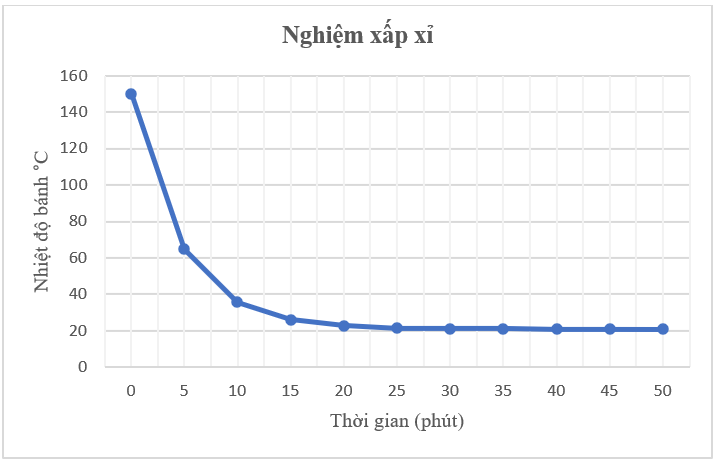
\includegraphics[scale=0.85]{Images/hinh_2_10.png}
	\caption[Biểu đồ nhiệt độ của bánh khi nguội đi trong bài tập Mục 2.4.1
	tính bằng phương pháp Euler tiến.
	]{\itshape\fontsize{13pt}{0pt}\selectfont\centering Biểu đồ nhiệt độ của bánh khi nguội đi trong bài tập Mục 2.4.1 tính bằng phương pháp Euler tiến.}
	\label{hinh2.10}
\end{figure}
\noindent Nhận xét: Dựa vào Bảng \ref{bang6} và Hình \ref{hinh2.10} ta thấy nhiệt độ bánh giảm đi theo thời gian. Trong khoảng 15 phút đầu nhiệt độ giảm khá nhanh, càng về sau giảm càng chậm và từ khoảng 35 phút trở đi, nhiệt độ bánh gần như trở về nhiệt độ~ phòng. 
\subsection{Mô hình hỗn hợp hai dung dịch muối}
\subsubsection{Xây dựng mô hình}
Trộn lẫn hai dung dịch muối có nồng độ khác nhau, lượng muối trong bể trộn tại thời điểm t sẽ được mô hình hóa bởi 1 phương trình vi phân, ta gọi 
${{R}_{in}}$ là tỷ lệ muối đầu vào, là lượng muối đi vào bể đo bằng số kg trong 1 phút (kg/min).\\
${{R}_{out}}$ là tỷ lệ muối đầu ra, là lượng muối bơm ra khỏi bể đo bằng kg/min.\\
${{r}_{in}}$ là tốc độ bơm vào của dung dịch nước muối đo bằng số lít trong 1 phút ($\ell$/min).\\
${{r}_{out}}$ là tốc độ bơm ra của dung dịch nước muối đo bằng $\ell$/min.\\
$c(t)$ là nồng độ muối trong bể tại thời điểm $t$ đo bằng số kg trong $1$ lít (kg/$\ell$).\\
Khi đó ${{R}_{in}}$ được tính bằng tích của nồng độ muối trong dung dịch bơm vào bể và tốc độ bơm vào của nước muối.\\
${{R}_{out}}$ được tính bằng tích của nồng độ muối trong dung dịch trong bể tại thời điểm t (là $c(t)$) và tốc độ bơm ra của nước muối.\\
$A(t)$ biểu thị lượng muối (đo bằng kg) trong bể tại thời điểm t.\\
 Khi đó tốc độ thay đổi của $A(t)$ là hiệu tỷ lệ muối đầu vào và tỷ lệ muối đầu ra, ta có bài toán giá trị ban đầu của mô hình là 
\begin{equation}
	 \left\{ \begin{array}{l}
 	 {A}'(t)={{R}_{in}}-{{R}_{out}}, \\ 
 	 A(0)={{A}_{0}}. \\ 
 \end{array} \right.
\label{eq:2.6}
\end{equation}
 \begin{figure}[H]
 	\centering
 	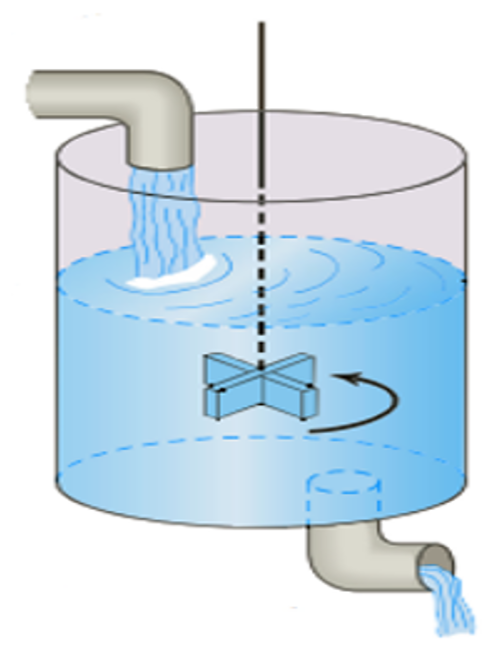
\includegraphics[scale=0.5]{Images/hinh_2_11.png}
 	\caption[Bể trộn dung dịch nước muối, xem \cite{ref4}. 
 	]{\itshape\fontsize{13pt}{0pt}\selectfont\centering Bể trộn dung dịch nước muối, xem \cite{ref4}.}
 	\label{hinh2.11}
 \end{figure}
\noindent\textbf{Ví dụ 2.5.1.} Giả sử rằng một bể trộn lớn ban đầu chứa $1000$ lít nước muối (trong đó có $20$ kg muối được hòa tan trong nước). Một dung dịch nước muối khác được bơm vào bể lớn với tốc độ 10 ($\ell$/min), nồng độ của muối trong dung dịch này là 0.3 (kg/$\ell$). Khi dung dịch trong bể được khuấy đều, nó được bơm ra cùng tốc độ với dung dịch đi vào. Tìm công thức A(t) tính lượng muối trong bể tại thời điểm t và tính lượng muối tại thời điểm t = 10 giây?\\
\textbf{Lời giải.}\\
Từ giả thiết ta tính được ${{r}_{in}}={{r}_{out}}=10\,$($\ell$/min), ${{R}_{in}}=\,0.3\,\times \,10\,=3$(kg/min), \newline ${{R}_{out}}=\dfrac{A(t)}{1000}\times 10\,=\dfrac{A(t)}{100}$(kg/min).\\
Ta có mô hình bài toán giá trị ban đầu là    
$\left\{ \begin{array}{l}
	 {A}'(t)=3-\dfrac{A(t)}{100}, \\ 
	 A(0)=20. \\ 
\end{array} \right.$\\
Áp dụng công thức (\ref{eq:1.8}) ta có
$$A(t)=20{{e}^{-\int\limits_{0}^{t}{\frac{1}{100}ds}}}+\int\limits_{0}^{t}{{{e}^{-\int\limits_{s}^{t}{\frac{1}{100}dz}}}3}\,ds\,\,=-280{{e}^{-\frac{1}{100}t}}+300\,\,\,.$$
Vậy công thức tính lượng muối trong bể tại thời điểm $t$ là $A(t)=300-280{{e}^{-\frac{1}{100}t}}\,.$\\
Tại thời điểm $t=10$ giây lượng muối trong bể là  $A(10)=46.64$ kg.\\
\textbf{Ví dụ 2.5.2.} Với giả thiết như trong Ví dụ 2.5.1, nếu dung dịch được khuấy đều và  được bơm ra với tốc độ chậm hơn, ${{r}_{out}}=7$ ($\ell$/min), tìm công thức tính $A(t)$? Vẽ đồ thị lượng muối trong bể, khi thời gian tăng lượng muối trong bể thay đổi như thế nào?\\
\textbf{Lời giải.}  
Ta có chất lỏng sẽ tích tụ trong bể với tốc độ là ${{r}_{in}}-{{r}_{out}}=10-7=3\, (\ell/min)$
Sau $t$ phút sẽ có $3t$ (lít) chất lỏng sẽ tích tụ trong bể, do đó bể sẽ chứa $(1000 + 3t)$ lít  nước muối. \\
Nồng độ của muối trong bể tại thời điểm $t$ là   $c(t)=\dfrac{A(t)}{1000+3t}\,$ (kg/$\ell$), và tỷ lệ đầu ra của muối là ${{R}_{out}}=c(t).\,{{r}_{out}}=\dfrac{A(t)}{1000+3t}\,\times 7\,=\dfrac{7A(t)}{1000+3t}\,$(kg/min).\\
Khi đó phương trình vi phân của mô hình trở thành ${A}'(t)=3-\dfrac{7A(t)}{1000+3t}.$\\
Áp dụng công thức (\ref{eq:1.8}) với $A(0)=20$ ta có 
$$A(t)=20{{e}^{-\int\limits_{0}^{t}{\frac{7}{1000+3s}ds}}}+\int\limits_{0}^{t}{{{e}^{-\int\limits_{s}^{t}{\frac{7}{1000+3z}dz}}}}.3ds $$
	$$ \Leftrightarrow A(t)=-{{28.10}^{8}}{{(1000+3t)}^{-\frac{7}{3}}}+300+0.9t. $$
Vậy công thức tính lượng muối trong bể tại thời điểm $t$ là $$A(t)=-\dfrac{{{28.10}^{8}}}{{{(1000+3t)}^{{}^{7}/{}_{3}}}}+300+0.9t.$$
Ta có $\underset{t\to +\infty }{\mathop{\lim }}\,A(t)=+\infty $, nghĩa là theo thời gian lượng muối trong bể ngày càng tăng lên đến vô cùng (quan sát Hình 2.12).
 \begin{figure}[H]
	\centering
	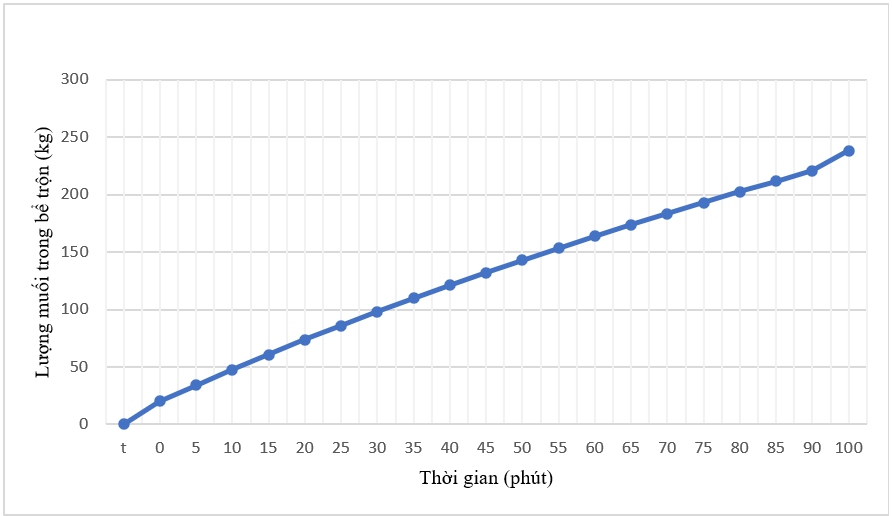
\includegraphics[scale=0.65]{Images/hinh_2_12.png}
	\caption[Đồ thị lượng muối có trong bể trộn trong Ví dụ 2.5.2.
	]{\itshape\fontsize{13pt}{0pt}\selectfont\centering Đồ thị lượng muối có trong bể trộn trong Ví dụ 2.5.2.}
	\label{hinh2.12}
\end{figure}
\noindent\textbf{Ví dụ 2.5.3.} Với giả thiết như Ví dụ 2.5.2, giả sử dung dịch muối được bơm ra với tốc độ 7 ($\ell$/min) và bể có một nắp mở và có tổng dung tích là 1300 lít.

 a) Khi nào bể chứa sẽ tràn ra?
 
 b) Số kg muối trong bể tại thời điểm tràn ra  sẽ là bao nhiêu?
 
 c) Giả sử rằng mặc dù bể đang tràn nước, dung dịch nước muối tiếp tục được bơm vào với tốc độ 10 ($\ell$/min) và dung dịch đã khuấy đều tiếp tục được bơm ra với tốc độ 7 ($\ell$/min). Hãy đưa ra phương pháp xác định số kg muối trong bể ở thời điểm t =150 phút.
 
  d) Vẽ đồ thị $A(t)$ khi $t$ thuộc $[0;200]$\\
\textbf{Lời giải. }\\
a) Ban đầu bể chứa 1000 lít dung dịch. Vì nước muối được bơm vào với tốc độ 10 ($\ell$/min) và hỗn hợp được bơm ra với tốc độ 7 ($\ell$/min), nên sự lượng dung dịch trong bể tăng $10-7=3$ ($\ell$/min).\\
Thời gian để nước trong bể tràn ra là $\dfrac{\left( 1300-1000 \right)}{3}=100$. \\
Vậy sau $100$ phút nước muối trong bể sẽ tràn ra.\\
b) Phương trình vi phân mô tả lượng muối trong bể là ${A}'(t)=3-\dfrac{7A}{1000+3t}$.\\
Theo kết quả của Ví dụ 2.5.2 ta có $$A(t)=-\dfrac{{{28.10}^{8}}}{{{(1000+3t)}^{{}^{7}/{}_{3}}}}\,\,\,+300+0,9t\,\,\,(0\le t\le 100)$$
Khi t=100 thì nước tràn ra, khi đó lượng muối trong bể là
$$A(100)=-\dfrac{{{28.10}^{8}}}{{{(1000+3\times 100)}^{{}^{7}/{}_{3}}}}\,+300+0.9\times 100=238.2\,(kg).\,\,\,\,\,$$
c) Khi bể đầy nước ta có tỷ lệ muối đầu vào và ra là
${{R}_{in}}=\,0.3\,\times \,10\,=3\,$(kg/min) và ${{R}_{out}}=\dfrac{A(t)}{1300}\times 7=\dfrac{7A(t)}{1300}$(kg/min).\\
Lượng muối trong bể được mô hình hóa sử dụng phương trình vi phân
$$\left\{ \begin{array}{l}
	 {A}'(t)=3-\dfrac{7A}{1300}, \\ 
	 \,A(100)=238.2. \\ 
\end{array} \right.$$
Áp dụng công thức (\ref{eq:1.8}) ta được
$$A(t)=238.2{{e}^{-\int\limits_{0}^{t}{\frac{7}{1300}ds}}}+\int\limits_{0}^{t}{{{e}^{-\int\limits_{s}^{t}{\frac{7}{1300}dz}}}.3}ds=-546.5{{e}^{-\frac{7t}{1300}}}+ \dfrac{3900}{7}$$
Vậy công thức tính lượng muối trong bể  tại thời điểm t là 
$$A(t)=-546.5{{e}^{-\frac{7t}{1300}}}+\dfrac{3900}{7}\,\,(t\ge 100)$$
Khi $t=150$ phút, lượng muối trong bể là  
$$A(150)=-546.5{{e}^{-\frac{7\times 150}{1300}}}+\dfrac{3900}{7}=313.5\,\,(kg)$$
d) đồ thị của $A(t)$ trên đoạn $\left[0, 200\right]$.
 \begin{figure}[H]
	\centering
	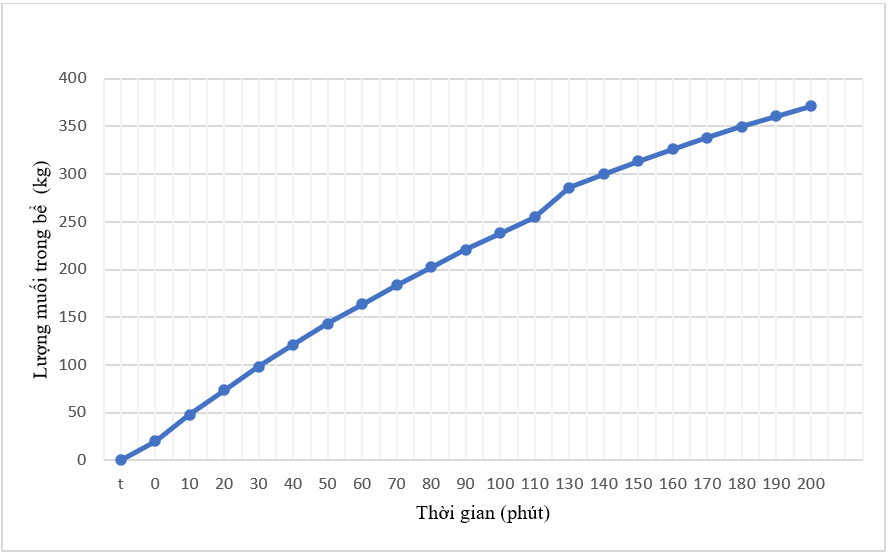
\includegraphics[scale=0.8]{Images/hinh_2_13.png}
	\caption[Đồ thị lượng muối có trong bể trong Ví dụ 2.5.3.
	]{\itshape\fontsize{13pt}{0pt}\selectfont\centering Đồ thị lượng muối có trong bể trong Ví dụ 2.5.3.}
	\label{hinh2.13}
\end{figure}
\subsubsection{Bài tập}
\noindent\textbf{Bài 2.5.1.}  Một bình chứa 200 lít dung dịch, trong đó có 30 gam muối được hòa tan. Nước muối có nồng độ 1 (g/$\ell$) sau đó được bơm vào bình với tốc độ 4 ($\ell$/min), dung dịch trộn đều được bơm ra với tốc độ như nhau. Tìm số gam muối A(t) trong bình tại thời điểm t.\\
\textbf{Lời giải. }\\
Ta có ${{R}_{in}}=1\times 4=4\,$(g/min) và ${{R}_{out}}=\dfrac{A(t)}{200}\times 4=\dfrac{A(t)}{50}\,$(g/min).\\
Mô hình là bài toán giá trị ban đầu  $\left\{ \begin{array}{l}
	 {A}'(t)=4-\dfrac{A(t)}{50}, \\ 
	 A(0)=30. \\ 
\end{array} \right.$\\
Giải phương trình vi phân ${A}'(t)=4-\dfrac{A(t)}{50}$, Áp dụng công thức (\ref{eq:1.8}) ta có
$$A(t)=30{{e}^{-\int\limits_{0}^{t}{\frac{1}{50}ds}}}+\int\limits_{0}^{t}{{{e}^{-\int\limits_{s}^{t}{\frac{1}{50}dz}}}.4}ds=-170{{e}^{-}}^{\frac{t}{50}}+200.$$
Vậy số gam muối trong bình tại thời điểm $t$ là $A(t)=-170{{e}^{-\frac{t}{50}}}+200$.\\
\textbf{Bài 2.5.2.} Với giả thiết như Bài 2.5.1,  giả sử rằng chỉ có nước tinh khiết được bơm vào bể, tìm số gam muối $A(t)$ trong bể tại thời điểm $t$?\\
\textbf{Lời giải.}\\
Nếu nước tinh khiết được bơm vào bể thì 
${{R}_{in}}=0\times 4=0\,$(g/min) \newline và ${{R}_{out}}=\dfrac{A(t)}{200}\times 4=\dfrac{A(t)}{50}\,$(g/min).\\
Mô hình là bài toán giá trị ban đầu  $\left\{ \begin{array}{l}
	 {A}'(t)=-\dfrac{A(t)}{50}, \\ 
	 A(0)=30. \\ 
\end{array} \right.$\\
Áp dụng công thức (\ref{eq:1.5}) ta có nghiệm của bài toán là $A(t)=30{{e}^{-\frac{t}{50}}}$.\\
Vậy số gam muối trong bể tại thời điểm $t$ là $A(t)=30{{e}^{-\frac{t}{50}}}$ .\\
\textbf{Bài 2.5.3.} Một bể lớn có dung tích chứa 1800 lít nước tinh khiết. Nước muối chứa 0.3 kg muối mỗi lít được bơm vào bể với tốc độ 20 ($\ell$/min). Dung dịch trộn đều được bơm ra với tốc độ bằng tốc độ bơm vào. Tìm công thức của A(t) là số kg muối trong bể tại thời điểm $t$.\\
\textbf{Lời giải.}\\
Theo giả thiết ta có ${{R}_{in}}=0.3\times 20=6\,$(kg/min) và ${{R}_{out}}=\dfrac{A(t)}{1800}\times 20=\dfrac{A(t)}{90}\,$(kg/min).\\
Mô hình là bài toán giá trị ban đầu $\left\{ \begin{array}{l}
	{A}'(t)=6-\dfrac{A(t)}{90}, \\ 
	 A(0)=0. \\ 
\end{array} \right.$\\
Áp dụng công thức (\ref{eq:1.8}) ta có nghiệm\\ $$A(t)=\int\limits_{0}^{t}{{{e}^{-\int\limits_{s}^{t}{\frac{1}{90}dz}}}.6}ds=-540{{e}^{-\frac{t}{90}}}+540.$$\\
Vậy lượng muối trong bể tại thời điểm t là $A(t)=-540{{e}^{-\frac{t}{90}}}+540$ .\\
\textbf{Bài 2.5.4. }Một bể lớn được lấp đầy một phần với 400 lít dung dịch, trong đó có 10 kg muối được hòa tan. Nước muối chứa 0.2 kg muối trong mỗi lít được bơm vào bể với tốc độ 20 ($\ell$/min). Dung dịch đã trộn kỹ sau đó được bơm ra với tốc độ 16 ($\ell$/min). Tìm số kg muối trong bể sau 30 phút.\\
\textbf{Lời giải. }\\
Tỷ lệ muối đầu vào là ${{R}_{in}}=0.2\times 20=4\,$(kg/min).\\
Do tốc độ bơm ra chậm hơn bơm vào nên mỗi phút lượng chất lỏng trong bể sẽ tăng thêm ${{r}_{in}}-{{r}_{out}}=20-16=4$ ($\ell$/min), sau t phút sẽ có 4t lít dung dịch sẽ tích tụ trong bể, do đó bể sẽ chứa (400 + 4t) lít nước muối. \\
Nồng độ của muối trong bể tại thời điểm t là $c(t)=\dfrac{A(t)}{400+4t}\,$(kg/$\ell$) và tỷ lệ đầu ra của muối là ${{R}_{out}}=c(t).\,{{r}_{out}}=\dfrac{A(t)}{400+4t}\,\times 16=\dfrac{16A(t)}{400+4t}\,\,=\dfrac{4A(t)}{100+t}\,$(kg/min).\\
Khi đó phương trình vi phân của mô hình trở thành $${A}'(t)=4-\dfrac{4A(t)}{100+t}\Leftrightarrow {A}'(t)=-\dfrac{4A(t)}{100+t}+4.$$
Áp dụng công thức (\ref{eq:1.8}) ta có nghiệm 
$$\begin{array}{lll}
A(t)&=10{{e}^{-\int\limits_{0}^{t}{\frac{4}{100+s}ds}}}+\int\limits_{0}^{t}{{{e}^{-\int\limits_{s}^{t}{\frac{4}{100+z}dz}}}.4}ds\\ &=\dfrac{-{{7.10}^{9}}}{{{(100+t)}^{4}}}+\dfrac{4}{5}(100+t)$$
\end{array}$$
Vậy công thức tính lượng muối trong bể tại thời điểm $t$ là $$A(t)=\dfrac{-7\times {{10}^{9}}}{{{(100+t)}^{4}}}+\dfrac{4}{5}(100+t).$$
Số kg muối trong bể sau 30 phút là $$A(30)=\dfrac{-7\times {{10}^{9}}}{{{(100+30)}^{4}}}+\dfrac{4}{5}(100+30)=79.5\,(kg)$$
\subsubsection{Mô phỏng bằng Excel.}
Xét Ví dụ 2.5.1: Giả sử rằng một bể trộn lớn ban đầu chứa $1000$ lít nước muối (trong đó có 20 kg muối được hòa tan nước). Một dung dịch nước muối khác được bơm vào bể lớn với tốc độ 10 ($\ell$/min), nồng độ của muối trong dung dịch này là 0.3 kg trên mỗi lít. Khi dung dịch trong bể được khuấy đều, nó được bơm ra với cùng tốc độ với dung dịch đi vào. \\
Công thức tính lượng muối trong bể tại thời điểm $t$ là $A(t)=-280{{e}^{-\frac{1}{100}t}}+300$.\\
Sử dụng tính gần đúng bằng phương pháp Euler tiến với $\,{{t}_{n}}={{t}_{0}}+nh$, $h=1.$\\  Áp dụng công thức Euler tiến (1.10) ${{A}_{n+1}}\approx \left( 1-\dfrac{h}{100} \right){{A}_{n}}+3h$, ta có bảng số liệu sau (ta chỉ trích xuất các giá trị tương ứng với các số thứ tự n chia hết cho 5).
\begin{table}[H]
	\centering
	\begin{tabularx}{\textwidth}{
			|>{\centering\arraybackslash}s
			|>{\centering\arraybackslash}s
			|>{\centering\arraybackslash}y
			|>{\centering\arraybackslash}y
			|>{\centering\arraybackslash}y
			|>{\centering\arraybackslash}y|
		}
		\hline
		\bfseries  n
		&\bfseries  $\mathbf{t}_{\mathbf{n}}$
		& \bfseries Nghiệm xấp xỉ
		& \bfseries Nghiệm chính xác
		& \bfseries Sai số 
		tuyệt đối
		& \bfseries Sai số 
		tương đối (\%)
		\\
		\hline
		0  & 0  & 20.000000 & 20.000000 & 0.000000 & 0.00000  \\ \hline
		5  & 5  & 33.722786 & 33.655761 & 0.067025 & 0.199148 \\ \hline
		10 & 10 & 46.773019 & 46.645523 & 0.127496 & 0.273330 \\ \hline
		15 & 15 & 59.183661 & 59.001767 & 0.181894 & 0.308286 \\ \hline
		20 & 20 & 70.986057 & 70.755389 & 0.230668 & 0.326008 \\ \hline
		25 & 25 & 82.210019 & 81.935781 & 0.274239 & 0.334699 \\ \hline
		30 & 30 & 92.883895 & 92.570898 & 0.312997 & 0.338116 \\ \hline
	\end{tabularx}
	\caption[Bảng số liệu lượng muối trong bể trộn trong Ví dụ 2.5.1.]{\itshape\fontsize{13pt}{0pt}\selectfont Bảng số liệu lượng muối trong bể trộn trong Ví dụ 2.5.1.}
	\label{bang7}
\end{table}
\begin{figure}[H]
	\centering
	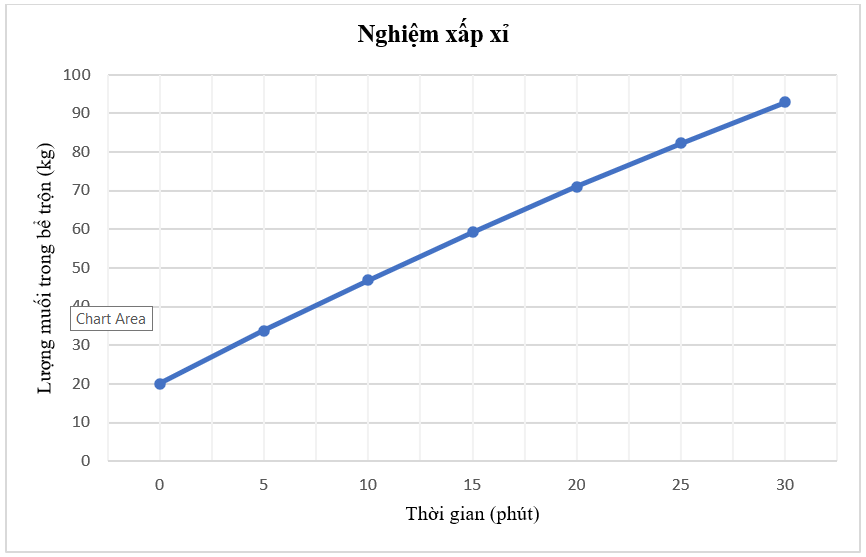
\includegraphics[scale=0.8]{Images/hinh_2_14.png}
	\caption[Biểu đồ lượng muối trong bể trộn trong Ví dụ 2.5.1
	tính bằng phương pháp Euler tiến.
	]{\itshape\fontsize{13pt}{0pt}\selectfont\centering Biểu đồ lượng muối trong bể trộn trong Ví dụ 2.5.1
		tính bằng phương pháp Euler tiến.}
	\label{hinh2.14}
\end{figure}
\subsection{Mô hình mạch điện mắc nối tiếp}
\subsubsection{Xây dựng mô hình}
\noindent\textbf{Trường hợp 1.  Đoạn mạch nối tiếp chỉ chứa một điện trở và một cuộn cảm.}\\
Cường độ dòng điện phụ thuộc vào biến $t$ là $I=I(t)$.\\
Điện áp giữa hai đầu cuộn cảm có độ tự cảm L là $L{I}'(t)$. \\
Điện áp giữa hai đầu điện trở có trở kháng R là $RI(t)$. \\
Theo định luật thứ hai của Kirchhoff  “Tổng giá trị điện áp dọc theo 1 vòng kín thì bằng 0” do đó điện áp  $E(t)$ đặt vào trên một vòng kín phải bằng tổng của các lần giảm điện áp trong vòng kín đó, điện áp $E(t)$ trên đoạn mạch là  
\begin{equation}
	L{I}'(t)+RI(t)=E(t)\Leftrightarrow {I}'(t)=-\dfrac{R}{L}I(t)+\dfrac{E(t)}{L}.
	\label{eq:2.7}
\end{equation}
Đây là phương trình vi phân tuyến  tính cho dòng điện $I(t)$.
\begin{figure}[H]
	\centering
	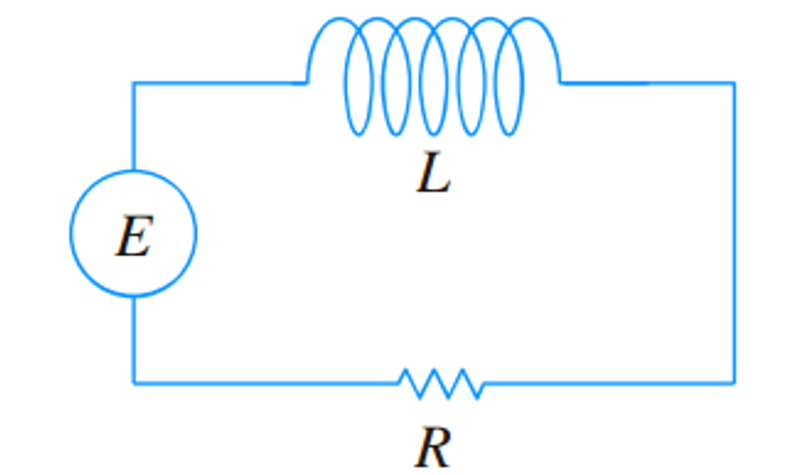
\includegraphics[scale=0.6]{Images/hinh_2_15.png}
	\caption[Mạch điện R, L mắc nối tiếp, xem \cite{ref4}.
	]{\itshape\fontsize{13pt}{0pt}\selectfont\centering Mạch điện R, L mắc nối tiếp, xem \cite{ref4}.}
	\label{hinh2.15}
\end{figure}
\noindent\textbf{Trường hợp 2. Đoạn mạch nối tiếp chỉ chứa một điện trở và một tụ điện.}\\
Điện áp trên tụ điện có điện dung C là $\dfrac{q(t)}{C}$ (trong đó $q(t)$ là điện tích trên tụ điện).
Khi đó theo định luật thứ hai của Kirchhoff điện áp $E(t)$ trên đoạn mạch là
\begin{equation}
	RI(t)+\dfrac{q(t)}{C}=E(t)    
	\label{eq:2.8}
\end{equation}                                    
\begin{figure}[H]
	\centering
	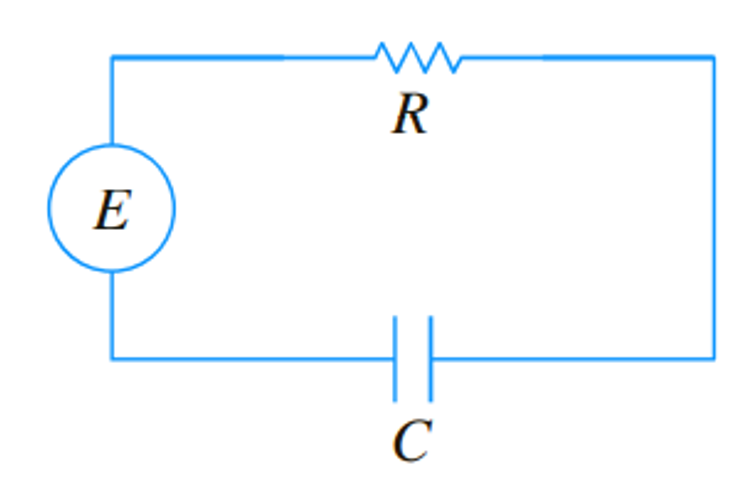
\includegraphics[scale=0.6]{Images/hinh_2_16.png}
	\caption[Mạch điện RC mắc nối tiếp, xem \cite{ref4}.
	]{\itshape\fontsize{13pt}{0pt}\selectfont\centering Mạch điện RC mắc nối tiếp, xem \cite{ref4}.}
	\label{hinh2.16}
\end{figure}
Mà $I(t)={q}'(t)$  nên phương trình (\ref{eq:2.8}) trở thành 
\begin{equation}
	Rq'(t)+\dfrac{q(t)}{C}=E(t)\Leftrightarrow q'(t)=-\dfrac{q(t)}{RC}+\dfrac{E(t)}{R}.  
	\label{eq:2.9}
\end{equation}                                
\textbf{Ví dụ 2.6.1.} Một pin $12$ Vôn được mắc thành mạch nối tiếp với 1 cuộn cảm có độ tự cảm là $\dfrac{1}{2}$ Henry và điện trở là 10 Omh. Xác định cường độ dòng điện I(t) nếu cường độ dòng điện ban đầu bằng 0? Tính cường độ dòng điện tại thời điểm t=0.1 giây, t=0.2 giây?\\
\textbf{Lời giải. }\\
Theo giả thiết E=12 (V), L=$\dfrac{1}{2}$ (H), R=10 (Omh).\\
Áp dụng công thức (\ref{eq:2.7}) và công thức nghiệm (\ref{eq:1.8}) với $I(0)=0$  ta có
$$ {I}'(t)=-\dfrac{R}{L}I(t)+\dfrac{E(t)}{L}\Leftrightarrow {I}'(t)=-20I+24 $$
$$\Leftrightarrow I(t)=\int\limits_{0}^{t}{{{e}^{-\int\limits_{s}^{t}{20dz}}}.24ds}\Leftrightarrow I(t)=-\dfrac{6}{5}{{e}^{-20t}}+\dfrac{6}{5}. $$
Vậy công thức tính cường độ dòng điện là $I(t)=\dfrac{6}{5} -\dfrac{6}{5}e^{-20t}$.\\
Khi $t=0.1s$, cường độ dòng điện là $I(0.1)=\dfrac{6}{5}-\dfrac{6}{5}e^{-2}=1.04 (A)$.\\
 Khi $t=0.2s$, cường độ dòng điện là   $I(0.2)=\dfrac{6}{5}-\dfrac{6}{5}e^{-4}=1.18 (A)$.  
\subsubsection{Bài tập}
\noindent\textbf{Bài 2.6.1.} Người ta đặt một suất điện động 30 Vôn vào một đoạn mạch LR, trong đó có độ tự cảm là 0.1 Henry và cảm kháng là 50 Omh. Tìm cường độ dòng điện I(t) nếu I(0)=0. Hãy xác định cường độ dòng điện khi $t\to +\infty $? \\
\textbf{Lời giải.} Theo giải thiết ta có E=30 (V), L=0,1 (H), R=50 (Omh)\\
Áp dụng công thức (\ref{eq:2.7}) và công thức nghiệm (\ref{eq:1.9}) với $I(0)=0$ ta được
$$ {I}'(t)=-\dfrac{R}{L}I(t)+\dfrac{E(t)}{L}\Leftrightarrow {I}'(t)=-500I+300 $$
	$$ \Leftrightarrow I(t)=\int\limits_{0}^{t}{{{e}^{-\int\limits_{s}^{t}{500dz}}}.300ds}\Leftrightarrow I(t)=\dfrac{3}{5}-\dfrac{3}{5}{{e}^{-500t}}. $$
Vậy công thức tính cường độ dòng điện là $I(t)=\dfrac{3}{5}-\dfrac{3}{5}{{e}^{-500t}}$   và  $\underset{t\to +\infty }{\mathop{\lim }}\,I(t)=\dfrac{3}{5}$. \newpage
\noindent\textbf{Bài 2.6.2.} Người ta đặt suất điện động $100$ Vôn vào đoạn mạch RC có trở kháng là $200$ Omh và điện dung là $10^{-4}$ Fara. Tìm điện tích $q(t)$ trên tụ nếu $q(0)=0$. Tìm cường độ dòng điện $I(t).$\\
\textbf{Lời giải. }\\
Theo giả thiết ta có $R=200$, $C={{10}^{-4}}$ , $E(t)=100$. Áp dụng công thức (\ref{eq:2.9}) ta được
$$q'(t)=-\dfrac{q(t)}{RC}+\dfrac{E(t)}{R}\Leftrightarrow q'(t)=-50q(t)+\dfrac{1}{2}.$$
Áp dụng công thức nghiệm (\ref{eq:1.9}) với $q(0)=0$ ta được
$$q(t)=\int\limits_{0}^{t}{{{e}^{-\int\limits_{s}^{t}{50dz}}}.\dfrac{1}{2}ds=}
-\dfrac{1}{100}{{e}^{-50t}}+\dfrac{1}{100}.$$
Vậy điện tích trên tụ là $q(t)=-\dfrac{1}{100}{{e}^{-50t}}+\dfrac{1}{100}$.\\
Do đó $I(t)=q'(t)=\dfrac{1}{2}{{e}^{-50t}}$.\\
\textbf{Bài 2.6.3.} Một suất điện động $200$ Vôn đặt vào một đoạn mạch RC có trở kháng là $1000$ Omh và điện dung là $5\times10^{-6}$ Fara. Tìm điện tích $q(t)$ trên tụ nếu $I(0)=0.4$. Xác định điện tích và cường độ dòng điện lúc $t= 0.005$ giây. Hãy xác định điện tích khi $t\to +\infty $ ?\\
\textbf{Lời giải.} Theo giả thiết $R=1000\,(\Omega ),\,\,\,C={{5.10}^{-6}}\,(F),\,\,\,E(t)=200\,(V)$.\\
Áp dụng công thức (\ref{eq:2.9}) và công thức nghiệm (\ref{eq:1.9}) ta có
$$ 
\begin{array}{lll}
&q'(t)&=-\dfrac{q(t)}{RC}+\dfrac{E(t)}{R}\Leftrightarrow q'(t)=-200q(t)+\dfrac{1}{5} \\
 \Leftrightarrow &q(t)&=C{{e}^{-\int{200}dt}}+{{e}^{-\int{200}dt}}\int{{{e}^{\int{200}dt}}.\dfrac{1}{5}dt} \\
\Leftrightarrow &q(t)&=C{{e}^{-200t}}+\dfrac{1}{1000}\Rightarrow I(t)={q}'(t)=-200C{{e}^{-200t}}.
\end{array}
$$
Ta lại có $I(0)=0.4$ nên $-50C=0.4\,\,$ hay $C=-\dfrac{1}{500}$. Vậy $I(t)=\dfrac{2}{5}{{e}^{-200t}}$.\\
Điện tích tại $t=0.005s$ là $q(t)=-\dfrac{1}{500}{{e}^{-200\times 0.005}}+\dfrac{1}{1000}=0.0003\,(c)$.\\
Cường độ dòng điện tại $t=0.005s$ là $I(0.005)=\dfrac{2}{5}{{e}^{-200\times 0.005}}=0.1472\,(A)$.\\
Ta có $q(t)=-\dfrac{1}{500}{{e}^{-200t}}+\dfrac{1}{1000}$ do đó $\underset{t\to +\infty }{\mathop{\lim }}\,q(t)=\dfrac{1}{1000}$.\\
\textbf{Bài 2.6.4.} Một suất điện động được xác định như sau
$E(t)=\left\{ \begin{array}{l}
	120\,\,\,khi\,\,\,0\,\le t\le 20, \\ 
	 0\,\,\,\,\,\,\,\,khi\,\,\,\,\,\,\,20<t. \\ 
\end{array} \right.$
được mắc vào mạch nối tiếp LR, trong đó độ tự cảm là $20$ (H) và điện trở là $2\,(\Omega )$ . Tìm cường độ dòng điện $I(t)$ tại thời điểm $t$ nếu $I(0)=0$.\\
\textbf{Lời giải. }\\
Theo giả thiết $L=20$ (H), $R=2(\Omega )$. \\
i)  Đối với $0\le t\le 20$ phương trình (\ref{eq:2.7}) có dạng 
$$ {I}'(t)=-\dfrac{R}{L}I(t)+\dfrac{E(t)}{L} $$
$$ \Leftrightarrow I'(t)=-\dfrac{1}{10}I(t)+6. $$
Áp dụng công thức nghiệm (\ref{eq:1.9}) với $I(0)=0$ ta có
$$I(t)=\int\limits_{0}^{t}{{{e}^{-\int\limits_{s}^{t}{\frac{1}{10}dz}}}.6}ds=60-60{{e}^{-\frac{t}{10}}}.$$
Tại $t =20$, ta có $I(20)=60-60{{e}^{-2}}$. \\
ii) Với $t >20$ phương trình (\ref{eq:2.7}) có dạng ${I}'(t)=-\dfrac{1}{10}I(t)$.\\
Áp dụng công thức nghiệm (\ref{eq:1.5}) ta có $$I(t)=I(20){{e}^{-\int\limits_{20}^{t}{\frac{1}{10}dz}}}=60{{e}^{2}}{{e}^{-\frac{t}{10}}}-60{{e}^{-\frac{t}{10}}}.$$
Vậy $I(t)=\left\{ \begin{array}{l}
	 60-60{{e}^{-\frac{t}{10}}},\,\,\,\,0\le t\le 20, \\ 
	 ({{e}^{2}}-1)60{{e}^{-\frac{t}{10}}},\,\,t>20. \\ 
\end{array} \right.$\\
\textbf{Bài 2.6.5.} Một đoạn mạch điện LR nối tiếp có cuộn cảm với độ tự cảm thay đổi được, độ tự cảm giảm dần theo công thức $L(t)=\left\{ \begin{array}{l}
	 1-\dfrac{1}{10}t $ khi $ 0\le t<10, \\ 
	 0\,\,\,\,\,\,\,\,\,\,\,\,\,\,\,\,\,\,\,\,\,\,\,\, $ khi $ \,\,\,\,\,t\ge 10. \\ 
\end{array} \right.\,\,$\\
Tìm cường độ dòng điện $I(t)$ nếu điện trở là $0.2 \Omega$, suất điện động là $E(t)=4$V và $I(0)=0$. Vẽ đồ thị hàm số $I(t)$?\\
\textbf{Lời giải. }\\
Khi $0\le t<10$  áp dụng công thức (\ref{eq:2.7}) và công thức nghiệm (\ref{eq:1.8}) với $I(0)=0$ ta có
$$  {I}'(t)=-\dfrac{R}{L}I(t)+\dfrac{E(t)}{L}\Leftrightarrow I'(t)=-\dfrac{2}{10-t}I+\dfrac{40}{10-t} $$
	$$ \Leftrightarrow I(t)=\int\limits_{0}^{t}{{{e}^{-\int\limits_{s}^{t}{\dfrac{2}{10-z}dz}}}.}\dfrac{40}{10-s}ds\Leftrightarrow I(t)=20-\dfrac{1}{5}{{(10-t)}^{2}}. $$
Vậy công thức tính $I(t)$ là $I(t)=-\dfrac{1}{5}{{(10-t)}^{2}}+20\,\,=-\dfrac{1}{5}{{t}^{2}}+4t\,\,(0\le t<10)$\\
Khi $t >10, L=0$ ta có phương trình (\ref{eq:2.7}) trở thành  $0.2I(t)=4\Leftrightarrow I(t)=20$.\\
Ta có đồ thị hàm số $I(t)$.
\begin{figure}[H]
	\centering
	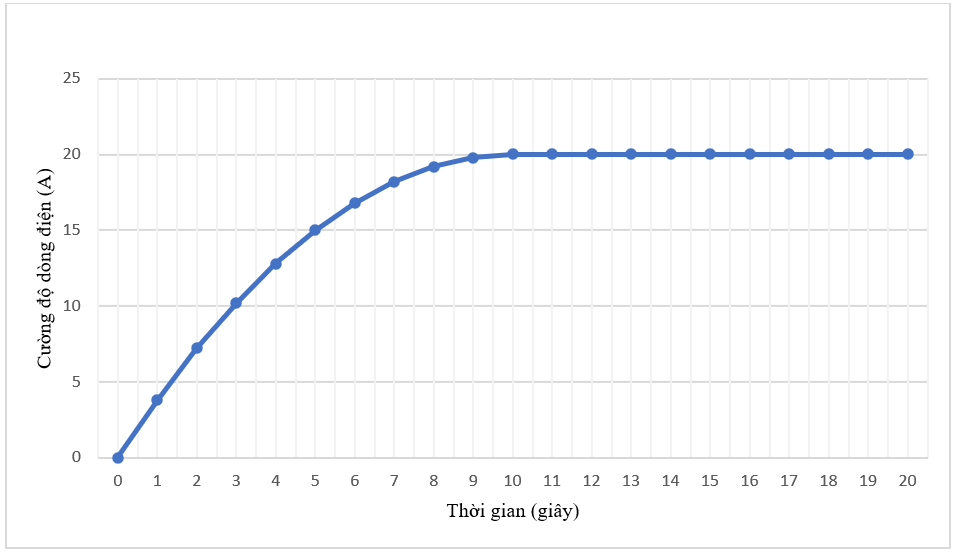
\includegraphics[scale=0.65]{Images/hinh_2_17.png}
	\caption[Đồ thị cường độ dòng điện I(t)
	]{\itshape\fontsize{13pt}{0pt}\selectfont\centering Đồ thị cường độ dòng điện I(t)}
	\label{hinh2.17}
\end{figure}
\subsubsection{Mô phỏng bằng Excel}
\noindent Xét lại Ví dụ 2.6.1:  Một pin $12$ Vôn được mắc thành mạch nối tiếp với 1 cuộn cảm có độ tự cảm là 1/2 Henry và điện trở là 10 Ohm. \\
Áp dụng công thức (\ref{eq:2.7}) ta có bài toán giá trị ban đầu $\left\{ \begin{array}{l}
	 I'(t)=24-20I, \\ 
	 I(0)=0. \\ 
\end{array} \right.$\\
Công thức nghiệm đúng của bài toán là $I(t)=\dfrac{6}{5}-\dfrac{6}{5}{e}^{-20t}$.\\
Sử dụng tính gần đúng bằng phương pháp Euler tiến với ${{t}_{n}}={{t}_{0}}+nh$ trong đó $h=0.01$, ${{I}_{n+1}}\approx (1-20h){{I}_{n}}+24h$, ta có bảng số liệu sau (ta chỉ trích xuất các giá trị trương ứng với số thứ tự n chia hết cho 5)
\begin{table}[H]
	\centering
	\begin{tabularx}{\textwidth}{
			|>{\centering\arraybackslash}s
			|>{\centering\arraybackslash}s
			|>{\centering\arraybackslash}y
			|>{\centering\arraybackslash}y
			|>{\centering\arraybackslash}y
			|>{\centering\arraybackslash}y|
		}
		\hline
			\bfseries  n
			&\bfseries  $\mathbf{t}_{\mathbf{n}}$
			& \bfseries Nghiệm xấp xỉ
			& \bfseries Nghiệm chính xác
			& \bfseries Sai số 
			tuyệt đối
			& \bfseries Sai số 
			tương đối (\%)
			\\
			\hline		
		5  & 0.05 & 0.806784    & 0.758544671 & 0.048239329 & 6.359457956 \\ \hline
		10 & 0.1  & 1.071150981 & 1.03759766  & 0.033553321 & 3.233750643 \\ \hline
		15 & 0.15 & 1.157778753 & 1.140255518 & 0.017523236 & 1.536781472 \\ \hline
		20 & 0.2  & 1.186164942 & 1.178021233 & 0.008143709 & 0.69130406  \\ \hline
		25 & 0.25 & 1.195466528 & 1.191914464 & 0.003552065 & 0.29801338  \\ \hline
		30 & 0.3  & 1.198514472 & 1.197025497 & 0.001488975 & 0.124389545 \\ \hline
		35 & 0.35 & 1.199513222 & 1.198905742 & 0.000607481 & 0.050669582 \\ \hline
	\end{tabularx}
	\caption[Bảng số liệu mô hình mạch điện mắc nối tiếp RL trong Ví dụ 2.6.1]{\itshape\fontsize{13pt}{0pt}\selectfont Bảng số liệu mô hình mạch điện mắc nối tiếp RL trong Ví dụ 2.6.1}
	\label{bang8}
\end{table}
\begin{figure}[H]
	\centering
	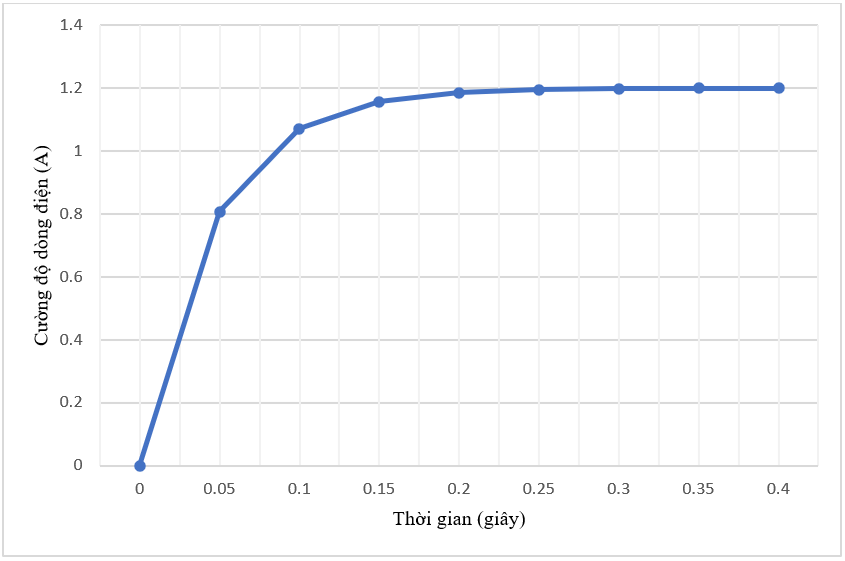
\includegraphics[scale=0.75]{Images/hinh_2_18.png}
	\caption[Biểu đồ cường độ dòng điện tức thời tại thời điểm t trong Ví dụ 2.6.1 tính bằng phương pháp Euler tiến.
	]{\itshape\fontsize{13pt}{0pt}\selectfont\centering Biểu đồ cường độ dòng điện tức thời tại thời điểm t trong Ví dụ 2.6.1 tính bằng phương pháp Euler tiến.}
	\label{hinh2.18}
\end{figure}

\noindent Nhận xét: Dựa vào bảng số liệu và biểu đồ ta thấy cường độ dòng điện ngày càng tăng theo thời gian. Đặc biệt từ 0 giây đến 0.1 giây tốc độ tăng khá nhanh, từ 0.1 giây trở đi tốc độ tăng chậm hơn. Tại t=0.1s và t=0.2s cường độ dòng điện có giá trị là xấp xỉ 0.071A và 0.186A, phù hợp với kết quả tính toán lý thuyết trong Ví dụ 2.6.1.
\subsection{Mô hình vật rơi trong không khí}
\subsubsection{Xây dựng mô hình}
\noindent \textbf{Trường hợp 1. Vật rơi không có lực cản của không khí. }

Để xây dựng một mô hình toán học về chuyển động của một vật thể dưới tác động của một lực ta sử dụng định luật chuyển động của Newton: “một vật thể sẽ đứng yên hoặc sẽ tiếp tục chuyển động với vận tốc không đổi trừ khi bị ngoại lực tác động”. Trong mỗi trường hợp, điều này tương đương với việc nói rằng khi tổng các lực tác dụng lên vật bằng không thì gia tốc a của vật bằng không. Định luật hai về chuyển động của Newton chỉ ra rằng khi lực tác dụng lên một vật khác 0, thì lực tỷ lệ với gia tốc a hay chính xác hơn là F = ma, trong đó m là khối lượng của vật đó.

Bây giờ, giả sử một tảng đá được ném xuống từ mái của một tòa nhà như minh họa trong Hình 2.19. Ta gọi s(t) là khoảng cách của hòn đá so với mặt đất tại thời điểm t. Gia tốc của hòn đá là đạo hàm cấp 2 của s(t) nghĩa là $a={s}''(t)$. 

Ta giả sử  hướng đi lên là dương và không có lực nào tác động lên đá ngoài lực hấp dẫn, thì theo định luật hai của Newton ta có  
\begin{equation}
	m{s}''(t)=-mg\Leftrightarrow {s}''(t)=-g.
\label{eq:2.10}
\end{equation}
Trong đó $g$ là gia tốc trọng trường. Nếu chiều cao của tòa nhà là $s_0$ và vận tốc ban đầu của tảng đá là ${{v}_{0}}$, thì $s$ được xác định từ bài toán giá trị ban đầu bậc hai~ là
\begin{equation}
	\left\{ \begin{array}{l}
	 {s}''(t)=-g, \\ 
	 s(0)={{s}_{0}}, \\ 
	 s'(0)=v(0)={{v}_{0}}. \\ 
\end{array} \right.\,
\label{eq:2.11}
\end{equation}
Từ phương trình (\ref{eq:2.10}) ta suy ra  
\begin{equation}
	s(t)=-\dfrac{1}{2}g{{t}^{2}}+{{v}_{0}}t+{{s}_{0}}.
\label{eq:2.12}
\end{equation}
\begin{figure}[H]
	\centering
	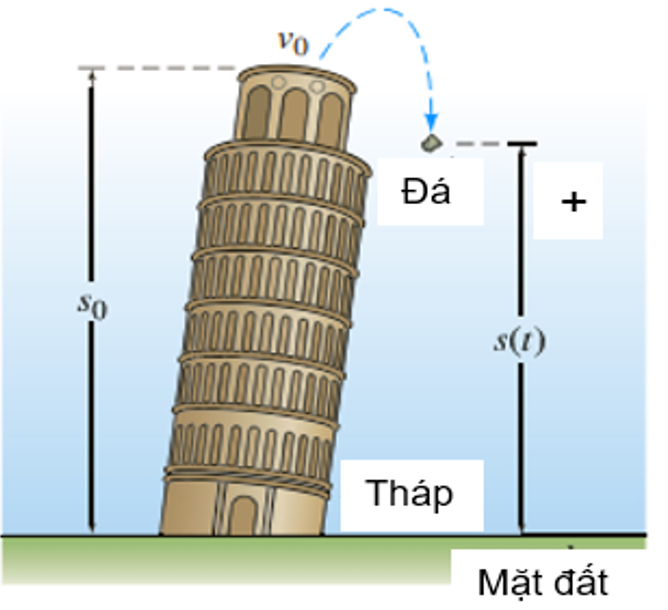
\includegraphics[scale=0.5]{Images/hinh_2_19.png}
	\caption[Vị trí của đá được đo từ mặt đất, xem \cite{ref4}.
	]{\itshape\fontsize{13pt}{0pt}\selectfont\centering Vị trí của đá được đo từ mặt đất, xem \cite{ref4}.}
	\label{hinh2.19}
\end{figure}                                       
\noindent\textbf{Trường hợp 2. Vật rơi có lực cản của không khí.}

Nhà toán học và vật lý người Ý Galileo Galilei (1564–1642) đã làm thí nghiệm thả vật rơi tự do từ tháp nghiêng Pisa, người ta thường tin rằng các vật nặng hơn chẳng hạn như một quả đạn pháo khi rơi tự do sẽ rơi với gia tốc lớn hơn các vật nhẹ hơn, chẳng hạn như như một chiếc lông vũ. Rõ ràng, một viên đạn pháo và một chiếc lông vũ khi được thả xuống đồng thời từ cùng một độ cao sẽ rơi với tốc độ khác nhau, nhưng không phải vì một viên đạn pháo nặng hơn mà nguyên nhân là do có lực cản của không khí. Lực cản không khí tỷ lệ với vận tốc tức thời $v(t)$.

Nếu ta coi chiều dương hướng xuống, thì lực tổng hợp tác dụng lên vật có khối lượng $\mathrm{m}$ sẽ là $F=F_1+F_2=m g-k v$, trong đó $F_1=m g$ là trọng lực tác dụng theo chiều dương và $F_2=-k v$ là lực cản không khí, tác động theo hướng ngược lại hay là hướng lên (xem Hình 2.20).
\begin{figure}[H]
	\centering
	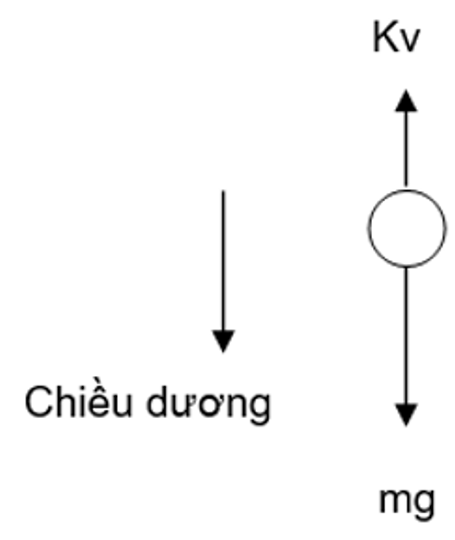
\includegraphics[scale=0.5]{Images/hinh_2_20.png}
	\caption[Vật rơi có khối lượng m
	]{\itshape\fontsize{13pt}{0pt}\selectfont\centering Vật rơi có khối lượng m}
	\label{hinh2.20}
\end{figure} 
Mặt khác vì $v(t)$ liên quan đến gia tốc $a$ bằng công thức  $a=v'(t)$, định luật hai của Newton trở thành $F=ma=mv'(t)$. Bằng cách cân bằng lực thực tế tác động vào vật  với dạng định luật hai này của Newton, chúng ta thu được phương trình vi phân bậc nhất cho vận tốc $v(t)$ của vật thể tại thời điểm $t$ là   
\begin{equation}
	mv'(t)=mg-kv\Leftrightarrow v'(t)=-\dfrac{k}{m}v+g.
\label{eq:2.13}
\end{equation}
với $k$ là hằng số tỷ lệ dương.
Nếu $s(t)$ là quãng đường vật rơi được trong thời gian $t$ kể từ thời điểm ban đầu 
thả thì $v={s}'(t)$do đó $a={v}'(t)={s}''(t)$. Thay vào (\ref{eq:2.13}) ta được phương trình vi phân 
cấp hai đối với $s(t)$ là  
\begin{equation}
	m{s}''(t)=mg-k{s}'(t)\,\,\Leftrightarrow \,m{s}''(t)+k{s}'(t)=mg.
\label{eq:2.14}
\end{equation}
Giả sử vận tốc ban đầu $v(0)={{v}_{0}}$ , ta có mô hình cho vật rơi trong không khí là phương trình vi phân bậc nhất đối với $v(t)$, chính là phương trình (\ref{eq:2.13}). Áp dụng công thức (\ref{eq:1.9}) ta có nghiệm của phương trình (\ref{eq:2.13}) như sau
$$ v(t)=v(0){{e}^{-\int\limits_{0}^{t}{\frac{k}{m}ds}}}+\int\limits_{0}^{t}{{{e}^{-\int\limits_{s}^{t}{\frac{k}{m}dz}}}.gds} $$
	$$\Leftrightarrow v(t)={{v}_{0}}{{e}^{-\int\limits_{0}^{t}{\frac{k}{m}ds}}}+\int\limits_{0}^{t}{{{e}^{-\int\limits_{s}^{t}{\frac{k}{m}dz}}}.gds} $$
	$$\Leftrightarrow v(t)={{e}^{-\frac{kt}{m}}}\left( {{v}_{0}}-\frac{mg}{k} \right)+\dfrac{mg}{k}. $$
Vậy nghiệm của bài toán giá trị ban đầu là 
\begin{equation}
	v(t)=\dfrac{mg}{k}+({{v}_{0}}-\dfrac{mg}{k}){{e}^{-\frac{kt}{m}}}.
\label{eq:2.15}
\end{equation}
Khi đó $\underset{t\to +\infty }{\mathop{\lim }}\,v(t)=\dfrac{mg}{k}$. Do ${s}'(t)=v,\,\,s(0)=0$ nên ta có công thức        
\begin{equation}
	s(t)=\dfrac{mg}{k}t-\dfrac{m}{k}({{v}_{0}}-\dfrac{mg}{k}){{e}^{-\frac{kt}{m}}}+\dfrac{m}{k}({{v}_{0}}-\dfrac{mg}{k}).
\label{eq:2.16}
\end{equation}
\subsubsection{Bài tập}
\noindent\textbf{Bài 2.7.1. }  Giả sử một viên đạn pháo nặng 7 kg được bắn thẳng đứng lên trên, như trong Hình 2.21, với vận tốc ban đầu $v_0=90$ m/s. \\
a) Giả sử bỏ qua lực cản của không khí. Nếu chiều dương hướng lên, thì mô hình chuyển động của viên đạn pháo được cho bởi ${s}''(t)=-g$  (phương trình (\ref{eq:2.9})của Mục 2.7.1). Vì ${s}'(t)=v(t)$ nên phương trình vi phân có dạng $v'(t)=-g$, trong đó ta lấy $g=9.8$ $m/s^2$. Tìm vận tốc $v(t)$ của quả đạn pháo tại thời điểm $t$, tính $v(5)$?\\
b) Sử dụng kết quả thu được ở phần a) để xác định độ cao $s(t)$ của quả đạn pháo được đo từ mặt đất. Tìm độ cao lớn nhất mà quả đạn pháo đạt được?\\
\begin{figure}[H]
	\centering
	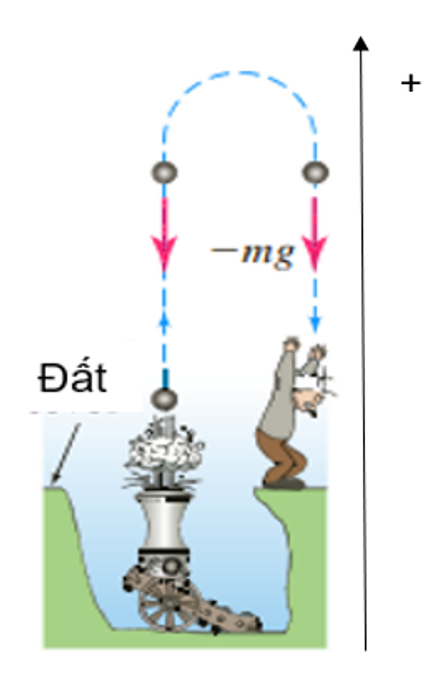
\includegraphics[scale=0.6]{Images/hinh_2_21.png}
	\caption[Viên đạn pháo được bắn lên từ mặt đất, xem \cite{ref4}.
	]{\itshape\fontsize{13pt}{0pt}\selectfont\centering Viên đạn pháo được bắn lên từ mặt đất, xem \cite{ref4}.}
	\label{hinh2.21}
\end{figure} 
\noindent\textbf{Lời giải}\\
a)  Từ phương trình $v'(t)=-g$ ta có $v(t)=-gt+C$.\\
Từ $\mathrm{v}(0)=90$ ta tìm được $\mathrm{C}=90$, và ta có $\mathrm{g}=9.8$, do đó vận tốc tức thời tại thời điểm $\mathrm{t}$ là $\mathrm{v}(\mathrm{t})=-9.8 \mathrm{t}+90$\\
Do đó khi $t=5s$, vận tốc là $v(5)=41 (m/s)$.\\
 b) Từ $\mathrm{v}(\mathrm{t})=-9.8 \mathrm{t}+90$ mà $s^{\prime}(t)=v(t)=-9.8 t+90 $ nên $ s(t)=-4.9 t^2+90 t+~C$.\\
Do $s(0)=0$ nên $C=0$ khi đó ta có $s(t)=-4.9{{t}^{2}}+90t.$\\
Độ cao cực đại đạt được khi $v=0$, ta có $-9.8t+90=0$ ta tính được $t=9.2 (s)$.\\
Khi đó chiều cao tối đa của quả đạn pháo so với mặt đất là    
$$s(9.2)=-4.9\times {{(9.2)}^{2}}+90\times 9.2=413.26\,(m)$$
\textbf{Bài 2.7.2.}  Bắn quả đạn pháo như trong Bài 2.7.1, nhưng lần này giả sử rằng lực cản của không khí tỷ lệ với vận tốc tức thời. Vì vậy độ cao tối đa mà quả đạn pháo đạt được phải nhỏ hơn độ cao quả đạn pháo trong phần (b) của Bài toán 2.6.1. Hãy chứng minh điều này bằng cách giả sử rằng hằng số tỉ lệ là $k=0.0025. $\\
\textbf{Lời giải.}\\
Khi lực cản của không khí tỷ lệ với vận tốc, áp dụng công thức (2.14) khi chiều dương hướng lên $$v(t)=\dfrac{mg}{k}+({{v}_{0}}-\dfrac{mg}{k}){{e}^{\frac{kt}{m}}}.$$
Áp dụng công thức (\ref{eq:2.16}) và sử dụng $s(0) = 0$ ta có
$$s(t)=\dfrac{mg}{k}t+\dfrac{m}{k}({{v}_{0}}-\dfrac{mg}{k}){{e}^{\frac{kt}{m}}}-\dfrac{m}{k}({{v}_{0}}-\dfrac{mg}{k}).$$
Đặt $k = 0.0025$, khối lượng $m =7, v(0) = 90 $ và $g = 9.8$  ta có
$$
\begin{array}{ll}
&s(t)=27440t-75972222{{e}^{0.00036t}}+75972222.\\
&v(t)=27440-27350{{e}^{0.00036t}}.
\end{array}
$$
Độ cao cực đại đạt được khi $v(t)=0\,\Leftrightarrow 27440-27350{{e}^{0.00036t}}=0\,\Leftrightarrow \,\,t=9\,$.\\ 
Khi đó chiều cao tối đa của quả đạn pháo sẽ là $s(9) = 410.8$ m, nhỏ hơn chiều cao tối đa khi không có lực cản không khí trong Bài 2.7.1 là $413.26$ m.\\
\textbf{Bài 2.7.3. } Một vận động viên nhảy dù nặng $60$ kg, còn chiếc dù và thiết bị của cô ấy cộng lại nặng 20 kg nữa. Sau khi thoát ra từ máy bay ở độ cao 4500 m, cô ấy đợi 15 giây và mở dù của mình. Giả sử rằng hằng số tỉ lệ có giá trị k=8 trong khi rơi tự do và k=160 sau khi dù được mở ra. Giả sử rằng vận tốc ban đầu của cô ấy khi rời máy bay bằng không. Vận tốc của cô ấy là bao nhiêu và cô ấy đã đi được quãng đường bao xa sau 20 giây kể từ khi rời máy bay? (xem Hình 2.22). Vận tốc của cô ấy lúc 20 giây như thế nào so với vận tốc lúc cuối của cô ấy? Cô ấy mất bao lâu để đến được mặt~ đất? 
\begin{figure}[H]
	\centering
	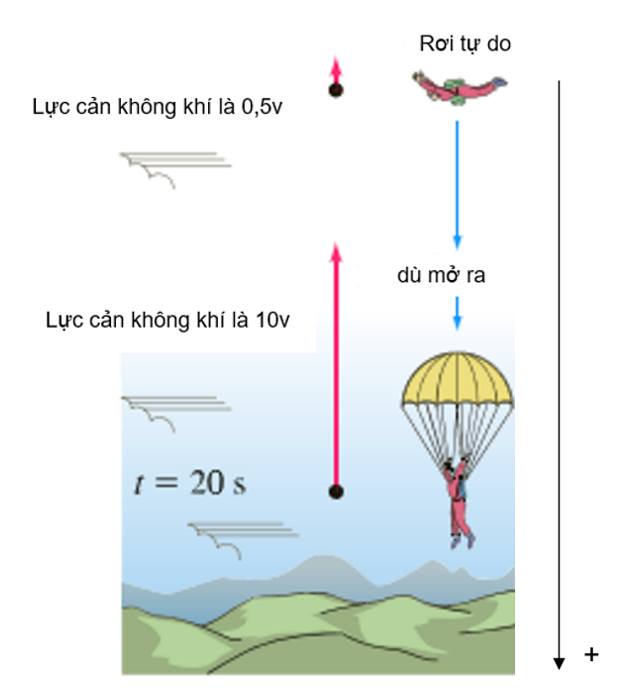
\includegraphics[scale=0.7]{Images/hinh_2_22.png}
	\caption[Minh họa cho bài toán nhảy dù, xem \cite{ref4}.
	]{\itshape\fontsize{13pt}{0pt}\selectfont\centering Minh họa cho bài toán nhảy dù, xem \cite{ref4}.}
	\label{hinh2.22}
\end{figure} 
\noindent\textbf{Lời giải}\\
Giả sử rằng lực cản của không khí tỉ lệ với vận tốc và chiều dương hướng xuống với $s(0) = 0$, mô hình cho vận tốc là công thức (\ref{eq:2.13}).\\
Áp dụng công thức (\ref{eq:2.14}) ta có $v(t)=\dfrac{mg}{k}+({{v}_{0}}-\dfrac{mg}{k}){{e}^{-\frac{kt}{m}}}$.\\
Vì vận tốc ban đầu ${{v}_{0}}=0$ nên $v(t)=\dfrac{mg}{k}+(-\dfrac{mg}{k}){{e}^{-\frac{kt}{m}}}=\dfrac{mg}{k}(1-{{e}^{-\frac{kt}{m}}})$.\\
i) Khi chưa mở dù  $k=8, m=60+20=80$ kg, $g=9.8m/{{s}^{2}}$ thay vào công thức tính vận 
tốc ta được ${{v}_{1}}(t)=98(1-{{e}^{-0.1t}})$ và ${{s}_{1}}(t)=98t+980{{e}^{-0.1t}}+{{C}_{1}}$. \\
Do ${{s}_{1}}(0)=0\Rightarrow {{C}_{1}}=-980\Rightarrow {{s}_{1}}(t)=98t+980{{e}^{-0.1t}}-980$. \\
Tại t=15s, vận tốc đạt được là ${{v}_{1}}(15)=76.13\,$(m/s). \\
Quãng đường đi được là ${{s}_{1}}(15)=708.67\,(m)$.\\
ii) Khi dù mở ra k=160,  vận tốc ban đầu bây giờ là ${{v}^{'}}_{0}={{v}_{1}}(15)=76.13$, thời gian tính từ lúc mở dù coi như t=0, s(0)=0. Áp dụng công thức (\ref{eq:2.14}) và (\ref{eq:2.15}) ta có 
$${{v}_{2}}(t)=\dfrac{mg}{k}+({{v}^{'}}_{0}-\dfrac{mg}{k}){{e}^{-\frac{kt}{m}}}=4.9+71.23{{e}^{-2t}}$$ và ${{s}_{2}}(t)=4.9t-35.615{{e}^{-2t}}+{{C}_{2}}.$\\
do $s(0)=0$ nên ${{C}_{2}}=35.615$ do đó ${{s}_{2}}(t)=4.9t-35.615{{e}^{-2t}}+35.615$.\\
Sau khi rời máy bay 20s, nghĩa là 5s sau khi dù bung ra, vận tốc của vận động viên nhảy dù là ${{v}_{2}}\left( 5 \right)=4.903$ (m/s) và quãng đường đi được là ${{s}_{2}}\left( 5 \right)=60.113\left( m \right).$\\
Vậy tính từ khi nhảy dù, vận tốc của vận động viên là v=4.903 (m/s).\\
Tổng quãng đường đi được là $s={{s}_{1}}+{{s}_{2}}=708.67+60.113=768.78\left( m \right)$\\
Vận tốc cuối của cô ấy là $\underset{t\to +\infty }{\mathop{\lim }}\,{{v}_{2}}(t)=4.9$(m/s), như vậy sau khi nhảy dù được 20s, vận động viên đã gần đạt đến vận tốc cuối cùng.\\
iii) Khoảng cách điểm nhảy dù so với mặt đất là 4500(m).\\
Tại thời điểm 15s sau khi mở chiếc dù ra, khoảng cách còn lại đến mặt đất là \newline
$4500-708.67=3791.33\,\,(m).$\\
Giải phương trình $$s_{2}(t)=3791.33\Leftrightarrow 4.9t-35.615{{e}^{-2t}}+35.615=3791.33~ t=~766.47.$$
Vậy thời gian từ lúc nhảy dù ra khỏi máy bay đến lúc tiếp cận mặt đất là \newline
$766.47+15=781.47(s)=13.0245$ phút.
\subsubsection{Mô phỏng bằng Excel}
Xét bài toán bắn viên đạn pháo (như trong Bài 2.7.2) với $g=9.8\,(m/{{s}^{2}})$, \newline$v_0=90$~ (m/s), 
m=7 kg, hệ số k=0.0025, chọn chiều dương hướng xuống.\\
Mô hình của chuyển động theo vận tốc tức thời là  
$$v'(t)=g-\dfrac{k}{m}v\Leftrightarrow v'(t)=9.8-0.00036v.$$
Công thức tính vận tốc tức thời là $v(t)=-27440+27350{{e}^{0.00036t}}.$\\
Sử dụng tính gần đúng bằng phương pháp Euler tiến với ${{t}_{n}}={{t}_{0}}+n.h$, $h=1.$ \newline Áp dụng công thức Euler tiến (\ref{eq:1.10}) ta có công thức tính nghiệm xấp xỉ\\
${{v}_{n+1}}\approx (1-0.00036h){{v}_{n}}+9.8h,$ ta có bảng số liệu sau (ta chỉ trích xuất các giá trị tương
ứng với số thứ tự n chia hết cho 5).
\begin{table}[H]
	\centering
	\begin{tabularx}{\textwidth}{
			|>{\centering\arraybackslash}s
			|>{\centering\arraybackslash}s
			|>{\centering\arraybackslash}y
			|>{\centering\arraybackslash}y
			|>{\centering\arraybackslash}y
			|>{\centering\arraybackslash}y|
		}
		\hline
		\bfseries  n
		&\bfseries   $\mathbf{t}_{\mathbf{n}}$
		& \bfseries Nghiệm xấp xỉ
		& \bfseries Nghiệm chính xác
		& \bfseries Sai số 
		tuyệt đối
		& \bfseries Sai số 
		tương đối (\%)
		\\
		\hline
		0  & 0  & -90         & -90         & 0           & 0            \\ \hline
		5  & 5  & -40.8733839 & -40.7256664 & 0.147717496 & -0.362713514 \\ \hline
		10 & 10 & 8.164867937 & 8.637440865 & 0.472572928 & 5.471214626  \\ \hline
		15 & 15 & 57.11491445 & 58.08948174 & 0.974567292 & 1.677700098  \\ \hline
		20 & 20 & 105.9769143 & 107.6306165 & 1.653702158 & 1.536460732  \\ \hline
		25 & 25 & 154.7510258 & 157.2610055 & 2.509979668 & 1.596059786  \\ \hline
		30 & 30 & 203.4374072 & 206.9808097 & 3.54340254  & 1.711947376  \\ \hline
		
	\end{tabularx}
	\caption[Bảng số liệu vận tốc tức thời viên đạn pháo trong Ví dụ 2.7.2.]{\itshape\fontsize{13pt}{0pt}\selectfont Bảng số liệu vận tốc tức thời viên đạn pháo trong Ví dụ 2.7.2.}
	\label{bang9}
\end{table}
\begin{figure}[H]
	\centering
	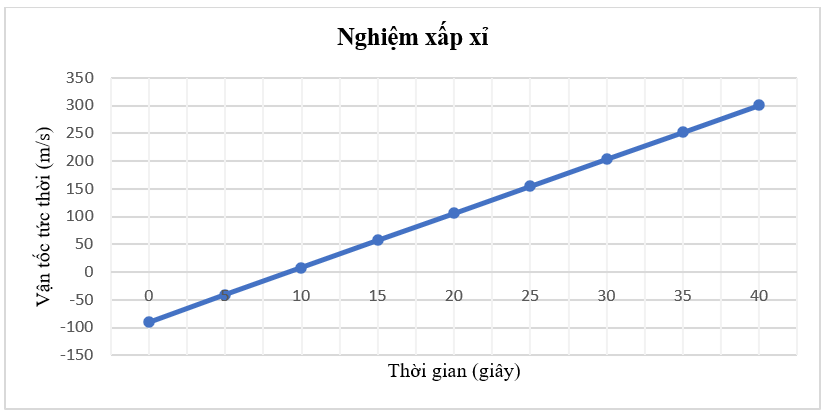
\includegraphics[scale=0.8]{Images/hinh_2_23.png}
	\caption[Biểu đồ vận tốc tức thời của quả đạn pháo trong Ví dụ 2.7.2 tính bằng phương pháp Euler tiến.
	]{\itshape\fontsize{13pt}{0pt}\selectfont\centering Biểu đồ vận tốc tức thời của quả đạn pháo trong Ví dụ 2.7.2 tính bằng phương pháp Euler tiến.}
	\label{hinh2.23}
\end{figure} 
\noindent\textbf{Nhận xét:} Dựa vào bảng số liệu và biểu đồ ta thấy ban đầu quả đạn pháo chuyển động lên trên (thể hiện bởi vận tốc mang dấu âm do chiều dương chọn hướng xuống),  vận tốc quả đạn pháo ngày càng giảm cho đến khi vận tốc bằng 0 thì quả đạn pháo chuyển động xuống mặt đất (thể hiện bởi vận tốc mang dấu dương) và lúc này vận tốc có giá trị tăng dần, quả đạn pháo chuyển động nhanh dần. Đạn pháo đạt độ cao lớn nhất (khi vận tốc bằng 0) vào khoảng hơn 9s sau khi ném (gần đúng với kết quả tính được ở Bài 2.7.1b là 9.2 giây).
\subsection{Mô hình chuyển động của tên lửa}
\subsubsection{Xây dựng mô hình}
\begin{figure}[H]
	\centering
	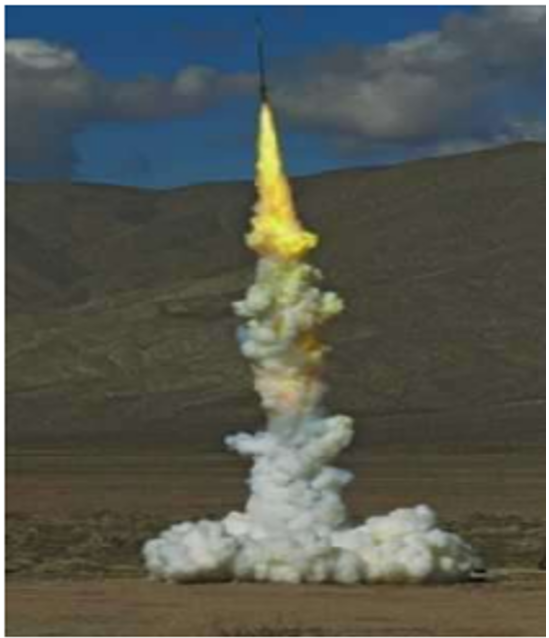
\includegraphics[scale=0.55]{Images/hinh_2_24.png}
	\caption[Tên lửa phóng thẳng đứng lên trời, xem \cite{ref4}.
	]{\itshape\fontsize{13pt}{0pt}\selectfont\centering Tên lửa phóng thẳng đứng lên trời, xem \cite{ref4}.}
	\label{hinh2.24.}
\end{figure} 
     Một tên lửa một tầng nhỏ được phóng thẳng đứng như Hình 2.24. Sau khi phóng, tên lửa tiêu thụ nhiên liệu, và do đó tổng khối lượng m(t) của nó thay đổi theo thời gian t (t > 0), v(t) là vận tốc tức thời tại thời điểm t.\\
Nếu giả thiết rằng chiều dương hướng lên, lực cản của không khí tỷ lệ với vận tốc tức thời v(t) của tên lửa theo hằng số k, và R là lực đẩy hoặc lực hướng lên được tạo ra bởi hệ thống đẩy.\\
Gọi ${{m}_{0}}$ là tổng khối lượng tên lửa tại thời điểm t=0 và $\lambda $ là tốc độ tiêu hao nhiên 
liệu, khi đó lượng nhiên liệu bị tiêu hao tại thời điểm t là $\lambda t$ và khối lượng nhiên 
liệu của tên lửa tại thời điểm t là $m(t)={{m}_{0}}-\lambda t$. \\
F là tổng lực tác dụng lên tên lửa, áp dụng định luật 2 của Newton khi khối lượng của vật thay đổi theo thời gian                             
\begin{equation}
	\begin{array}{ll}
	 F&=(mv{)}'(t)=v{m}'(t)+m{v}'(t) \\ 
	&=v({{m}_{0}}-\lambda t{)}'(t)+({{m}_{0}}-\lambda t){v}'(t) \\ 
	 &=-v\lambda +({{m}_{0}}-\lambda t){v}'(t).
\end{array}
\label{eq:2.17}
\end{equation}
Mặt khác tổng lực tác dụng lên tên lửa là
\begin{equation}
	F=-gm(t)+R-kv=-g({{m}_{0}}-\lambda t)+R-kv
\label{eq:2.18}
\end{equation}
Từ (\ref{eq:2.17}) và (\ref{eq:2.18}) ta có
\[\begin{array}{l}
	 -v\lambda +({{m}_{0}}-\lambda t)v'(t)=-g({{m}_{0}}-\lambda t)+R-kv \\ 
	 \Leftrightarrow ({{m}_{0}}-\lambda t)v'(t)+(k-\lambda )v=-g({{m}_{0}}-\lambda t)+R \\ 
	 \Leftrightarrow v'(t)=-\dfrac{(k-\lambda )}{({{m}_{0}}-\lambda t)}v-g+\dfrac{R}{({{m}_{0}}-\lambda t)}. \\ 
\end{array}\]
Vậy mô hình cho vận tốc tức thời của tên lửa là 
\begin{equation}
	v'(t)=-\dfrac{(k-\lambda )}{({{m}_{0}}-\lambda t)}v-g+\dfrac{R}{({{m}_{0}}-\lambda t)} \ .
\label{eq:2.19}
\end{equation}
\subsubsection{Bài tập}
\noindent \textbf{Bài 2.8.1.} Với giả thiết như Mục 2.8.1 biết ${{m}_{0}}=200\,kg\,,\,\,R=2000\,N,\,\,\lambda =1\,kg/s,\,\,$ $g=9.8\,\,m/{{s}^{2}},\,\,k=3\,\,kg/s,\,\,v(0)=0$.\\
a) Tìm vận tốc v(t) của tên lửa, tính vận tốc tại t=10 giây, 20 giây?\\
b) Tính độ cao s(t) của tên lửa tại thời điểm t. \\
\textbf{Lời giải.}
a) Với các giá trị được đưa ra trong đề bài, bài toán giá trị ban đầu trở thành
$$\left\{ \begin{array}{l}
	 v'(t)=-\dfrac{2}{200-t}v-9.8+\dfrac{2000}{200-t}, \\ 
 v(0)=0. \\ 
\end{array} \right.$$
Áp dụng công thức (\ref{eq:1.9}) ta có nghiệm của bài toán là
\[\begin{array}{lll}
	 &v(t)&=v(0){{e}^{-\int\limits_{0}^{t}{\frac{2}{200-s}ds}}}+\int\limits_{0}^{t}{{{e}^{-\int\limits_{s}^{t}{\frac{2}{200-z}dz}}}}.\left( -9.8+\dfrac{2000}{200-s} \right)ds \\ 
	 \Leftrightarrow &v(t)&=\int\limits_{0}^{t}{{{e}^{-\int\limits_{s}^{t}{\frac{2}{200-z}dz}}}}.\left( -9.8+\dfrac{2000}{200-s} \right)ds \\ 
	 \Leftrightarrow &v(t)&=0.024{{(200-t)}^{2}}+9.8t-960. \\ 
\end{array}\]
Như vậy vận tốc tên lửa tại thời điểm t là
$$v(t)=0.024{{(200-t)}^{2}}+9.8t-960=0.024{{t}^{2}}+0.2t \ .$$
Vận tốc của tên lửa tại $t=10$ giây là $v(10)=4.4$ (m/s).\\
Vận tốc của tên lửa tại $t=20$ giây là $v(20)=13.6$ (m/s).\\
b) Do ${s}'(t)=v(t)$nên $s(t)=\int{v(t)dt}=0.008{{t}^{3}}+0.1{{t}^{2}}+{{C}_{1}}.$\\
Ta giả sử đo độ cao của tên lửa từ mặt đất là s = 0, ta có s(0) = 0 nên $C_1 = 0$.\\
Khi đó độ cao của tên lửa tại thời điểm t là $s(t)=0.008{{t}^{3}}+0.1{{t}^{2}}$.\\
\textbf{Bài 2.8.2.} Phóng một tên lửa với giả thiết như trong Bài toán 2.8.1, giả sử khối lượng ban đầu của tên lửa là $m_0$ và khối lượng của nhiên liệu là 50 kg.\\
a) Thời gian tiêu hao $t_b$ hay thời gian mà tất cả nhiên liệu được tiêu thụ là bao nhiêu?\\
b) Vận tốc của tên lửa lúc đốt hết nhiên liệu là bao nhiêu?\\
c) Độ cao của tên lửa lúc đốt hết nhiên liệu là bao nhiêu?\\
d) Tại sao ta mong đợi tên lửa đạt được độ cao lớn hơn con số trong phần b)?\\
e) Sau khi đốt cháy hết nhiên liệu, một mô hình toán học cho vận tốc của tên lửa là~ gì?\\
\textbf{Lời giải.}\\
a) Gọi $t_b$ là thời gian mà tất cả nhiên liệu được tiêu thụ hết và ${{m}_{f}}(t)$là lượng nhiên liệu tiêu thụ đến thời điểm t. Theo giả thiết ${{m}_{f}}(0)=50\,kg$, tốc độ tiêu thụ nhiên liệu $\lambda =1\,\,(kg/s)$. Khi đó thời gian tên lửa cháy hết nhiên liệu là ${{t}_{b}}=\dfrac{{{m}_{f}}(0)}{\lambda }=\dfrac{50}{1}=50\,(s).$\\
b) Tại thời điểm cháy hết nhiên liệu t=50 giây, khi đó vận tốc tên lửa là
$$v(t)=0.024{{t}^{2}}+0.2t=0.024{{(50)}^{2}}+0.2\times 50=70.$$
c) Độ cao của tên lửa lúc đốt cháy hết nhiên liệu là 
$$s(t)=0.008{{t}^{3}}+0.1{{t}^{2}}=0.008{{(50)}^{3}}+0.1{{(5)}^{2}}=1250\,(m).$$
d) Khi đốt cháy hết nhiên liệu tên lửa sẽ có động lượng hướng lên sẽ đưa nó lên cao~ hơn.\\
e) Sau khi đốt cháy hết nhiên liệu, tổng khối lượng của tên lửa là một hằng số bằng 200 - 50 = 150 kg. \\
Khi đó áp dụng định luật hai Newton với vật có khối lượng không đổi, tổng lực tác dụng lên tên lửa là $F=mv'(t)$.\\
Chọn chiều dương hướng lên, các lực tác dụng vào tên lửa bao gồm lực cản không 
khí, trọng lực của trái đất, lực đẩy tạo ra bởi hệ thống đẩy, ta có
$$mv'(t)=-kv-mg+R.$$
Ta xác định được m = 150, k = 3, g = 9.8  và R = 0, vì lực đẩy bằng 0 sau khi đốt cháy nhiên liệu, do đó mô hình toán học cho vận tốc của tên lửa là 
$$150v'(t)=-3v-150(9.8)+0\Leftrightarrow v'(t)=-\dfrac{v}{50}-9.8.$$
\subsubsection{Mô phỏng bằng Excel}
\noindent Xét Bài toán 2.8.1 cho bởi mô hình sau 
$\left\{ \begin{array}{l}
	 v'(t)=-\dfrac{2}{200-t}v-9.8+\dfrac{2000}{200-t}, \\ 
	 v(0)=0. \\ 
\end{array} \right.$\newline
Công thức nghiệm đúng tính vận tốc tức thời của tên lửa là: $v(t)=0.024{{t}^{2}}+0.2t.$\\
Sử dụng tính gần đúng bằng phương pháp Euler tiến với ${{t}_{n}}={{t}_{0}}+nh$, bước nhảy h=1,
áp dụng công thức (\ref{eq:1.10}) ${{v}_{n+1}}\approx \left( 1-\dfrac{2h}{200-{{t}_{n}}} \right){{v}_{n}}+h\left( -9.8+\dfrac{2000}{200-{{t}_{n}}} \right)$, ta có bảng số liệu sau (ta chỉ trích xuất số liệu ứng với số thứ tự n chia hết cho 5)
\begin{table}[H]
	\centering
	\begin{tabularx}{\textwidth}{
			|>{\centering\arraybackslash}s
			|>{\centering\arraybackslash}s
			|>{\centering\arraybackslash}y
			|>{\centering\arraybackslash}y
			|>{\centering\arraybackslash}y
			|>{\centering\arraybackslash}y|
		}
		\hline
		\bfseries  n
		&\bfseries   $\mathbf{t}_{\mathbf{n}}$
		& \bfseries Nghiệm xấp xỉ
		& \bfseries Nghiệm chính xác
		& \bfseries Sai số 
		tuyệt đối
		& \bfseries Sai số 
		tương đối (\%)
		\\
		\hline
		0  & 0  & 0           & 0    & 0           & 0           \\ \hline
		5  & 5  & 1.48241206  & 1.6  & 0.11758794  & 7.349246231 \\ \hline
		10 & 10 & 4.170854271 & 4.4  & 0.229145729 & 5.207857469 \\ \hline
		15 & 15 & 8.065326633 & 8.4  & 0.334673367 & 3.984206748 \\ \hline
		20 & 20 & 13.16582915 & 13.6 & 0.434170854 & 3.192432752 \\ \hline
		25 & 25 & 19.47236181 & 20   & 0.527638191 & 2.638190955 \\ \hline
		30 & 30 & 26.98492462 & 27.6 & 0.615075377 & 2.228533974 \\ \hline
		35 & 35 & 35.70351759 & 36.4 & 0.696482412 & 1.91341322  \\ \hline
		40 & 40 & 45.6281407  & 46.4 & 0.771859296 & 1.663489863 \\ \hline
	\end{tabularx}
	\caption[Bảng số liệu vận tốc tức thời của tên lửa trong Bài toán 2.8.1.]{\itshape\fontsize{13pt}{0pt}\selectfont Bảng số liệu vận tốc tức thời của tên lửa trong Bài toán 2.8.1.}
	\label{bang10}
\end{table}
\begin{figure}[H]
	\centering
	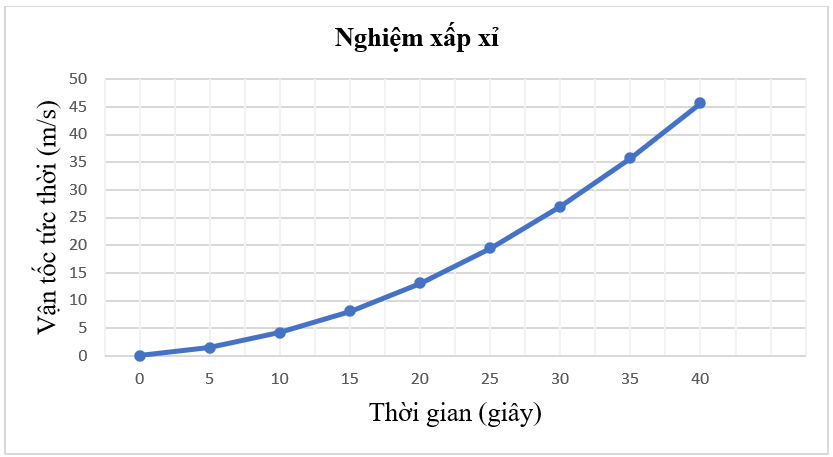
\includegraphics[scale=0.9]{Images/hinh_2_25.png}
	\caption[Biểu đồ vận tốc tức thời của tên lửa trong Bài toán 2.8.1 tính bằng phương pháp Euler tiến.
	]{\itshape\fontsize{13pt}{0pt}\selectfont\centering Biểu đồ vận tốc tức thời của tên lửa trong Bài toán 2.8.1 tính bằng phương pháp Euler tiến.}
	\label{hinh2.25}
\end{figure} 
\subsection{Mô hình hộp trượt trên mặt phẳng nghiêng}
\subsubsection{Xây dựng mô hình}
\begin{figure}[H]
	\centering
	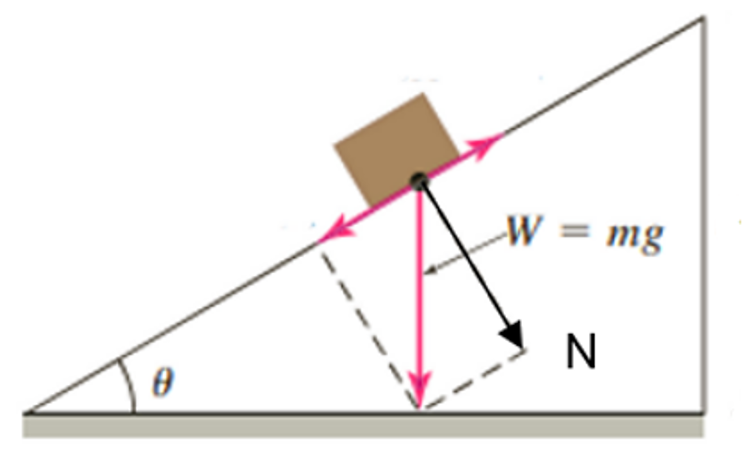
\includegraphics[scale=0.6]{Images/hinh_2_26.png}
	\caption[Hộp trượt trên mặt phẳng nghiêng, xem \cite{ref4}.
	]{\itshape\fontsize{13pt}{0pt}\selectfont\centering Hộp trượt trên mặt phẳng nghiêng, xem \cite{ref4}.}
	\label{hinh2.26}
\end{figure} 
\noindent Một hộp khối lượng m trượt xuống một mặt phẳng nghiêng tạo với phương ngang một góc $\theta $ như Hình 2.27. Gọi v(t) là vận tốc tức thời tại thời điểm t, chọn gốc tọa độ ở vị trí cao nhất, chiều dương cùng chiều với hướng chuyển động, v(0)=0, s(0)=0. Ta sẽ đi tìm phương trình vi phân cho vận tốc v(t) trong ba trường hợp sau. \\
\textbf{Trường hợp 1. }Không có ma sát trượt và không có lực cản của không khí.
Khi đó lực tác dụng lên hộp chỉ có trọng lực, chiếu lên phương chuyển động có độ lớn là $mg\sin \theta $.\\
Sử dụng định luật hai của Newton ta có $F=ma=mv'(t)$.\\
Phương trình vi phân của vận tốc v(t) là 
\begin{equation}
	mv'(t)=mg\sin \theta \,\,hay\,\,\,v'(t)=g\sin \theta 
\label{eq:2.20}
\end{equation}
\textbf{Trường hợp 2. } Có ma sát trượt và không có lực cản của không khí.\\
Lực ma sát trượt là lực hãm tác dụng ngược lại với hướng chuyển động.\\
Với $\mu $là hệ số ma sát trượt,  N là thành phần pháp tuyến của trọng lượng của hộp, khi đó $N=mg\cos \theta $, lực ma sát trượt có độ lớn là $\mu mg\cos \theta $. Mô hình trở thành       
\begin{equation}
	mv'(t)=mg\sin \theta -\mu mgcos\theta \Leftrightarrow v'(t)=g\sin \theta -\mu gcos\theta .\,\,
\label{eq:2.21}
\end{equation}
\textbf{Trường hợp 3.}  Có lực ma sát trượt và lực cản của không khí\\
Lực ma sát trượt có độ lớn là $\mu mg\cos \theta $.\\
Lực cản của không khí tỷ lệ thuận với vận tốc tức thời, ngược hướng với hướng chuyển động. Độ lớn lực cản không khí là $kv$, trong đó k>0 là hệ số của lực cản. Mô hình của chuyển động là                                    
\begin{equation}
	\begin{array}{ll}
	&m{v}'(t)=mg\sin \theta -\mu gcos\theta -kv \\ 
	\Rightarrow &{v}'(t)=g\sin \theta -\mu gcos\theta -\dfrac{kv}{m}.
\end{array}
\label{eq:2.22}
\end{equation}
\subsubsection{Bài tập}
\noindent\textbf{Bài 2.9.1.} Xét hộp trượt như trong Mục 2.9.1, giả sử rằng chiếc hộp nặng 50 kg, góc nghiêng của mặt phẳng là $\theta ={{30}^{o}}$ hệ số của ma sát trượt là $\mu =\dfrac{\sqrt{3}}{4}$ ,và hệ số lực cản không khí là $k=\dfrac{m}{4}$. Hãy giải phương trình vi phân trong ba trường hợp trên, giả sử rằng hộp bắt đầu từ trạng thái nghỉ từ điểm cao nhất cách mặt đất 15m.\\
\textbf{Lời giải}\\
\textbf{Trường hợp 1.}  Không có ma sát trượt, không có lực cản không khí.\\
Phương trình vi phân (2.20) trở thành
$$v'(t)=g\sin {{30}^{o}}=g\dfrac{1}{2}\Rightarrow v(t)=\dfrac{gt}{2}+{{C}_{1}}.$$
Vì $v(0)=0 $ nên ${{C}_{1}}=0$. Khi đó $v(t)=\dfrac{gt}{2}=4.9t$.\newpage
\noindent\textbf{Trường hợp 2.} Có ma sát trượt và không có lực cản không khí.\\
Phương trình vi phân (\ref{eq:2.21}) trở thành
$$v'(t)=g\sin \theta -\mu gcos\theta =g\times \dfrac{1}{2}-\dfrac{\sqrt{3}}{4}\times g\times \dfrac{\sqrt{3}}{2}=\dfrac{g}{8}\Rightarrow v(t)=\dfrac{gt}{8}+{{C}_{2}}.$$
Do $v(0)=0$ nên ${{C}_{2}}=0$. Vậy $v(t)=\dfrac{g}{8}t$.\\
\textbf{Trường hợp 3.}  Khi có lực ma sát trượt và lực cản không khí.\\
Phương trình vi phân (\ref{eq:2.22}) trở thành
$$\begin{array}{ll}
	 v'(t)&=g\sin \theta -\mu gcos\theta -\dfrac{kv}{m}\,\,\, \\ 
	 &=g\sin {{30}^{o}}-\dfrac{\sqrt{3}}{4}g\cos {{30}^{o}}-\dfrac{v}{4} \\ 
	 &=\dfrac{g}{2}-\dfrac{3g}{8}-\dfrac{v}{4}=-\dfrac{v}{4}+\dfrac{g}{8}. \\ 
\end{array}$$
Giải phương trình vi phân trên áp dụng công thức (\ref{eq:1.8}) với $v(0)=0$ ta được nghiệm $$v(t)=\int\limits_{0}^{t}{{{e}^{-\int\limits_{s}^{t}{\frac{1}{4}dz}}}.\dfrac{g}{8}ds}=\dfrac{g}{2}-\dfrac{g}{2}.{{e}^{-\frac{t}{4}}}.$$
Vậy $v(t)=\dfrac{g}{2}-\dfrac{g}{2}.{{e}^{-\frac{t}{4}}}=4.9-4.9{{e}^{-0.25t}}.$ \\
Vận tốc của hộp tại $t=10$ giây là $v(10)=4.5 $ (m/s).\\
Vận tốc của hộp tại $t=20$ giây là $v(20)=4.867$ (m/s).\\ 
\noindent\textbf{Bài 2.9.2. }\\
a) Trong Bài 2.9.1, gọi s(t) là khoảng cách đo được đến chân mặt phẳng nghiêng từ điểm cao nhất. Tính thời gian để hộp trượt hoàn toàn xuống chân mặt phẳng nghiêng. \\
b) Trong trường hợp có ma sát $\left( \mu \ne 0 \right)$nhưng không có lực cản của không khí, giải thích tại sao hộp không trượt trên mặt phẳng bắt đầu từ điểm cao nhất khi góc nghiêng $\theta $ thỏa mãn $\tan \theta \le \mu $.\\
c) Hộp sẽ trượt trên mặt phẳng khi $\tan \theta \le \mu $ nếu nó được truyền một vận tốc ban đầu $v(0)={{v}_{0}}>0$. Giả sử rằng $\mu =\dfrac{\sqrt{3}}{4}\,\,\,v\grave{a}\,\,\,\theta ={{23}^{o}}$, chứng minh rằng $\tan \theta \le \mu $. Hộp sẽ trượt trên mặt phẳng quãng đường bao xa nếu ${{v}_{0}}=0.3$(m/s)?\\
d) Sử dụng các giá trị $\mu =\dfrac{\sqrt{3}}{4}\,\,\,v\grave{a}\,\,\,\theta ={{23}^{o}}$, tính gần đúng vận tốc ban đầu ${{v}_{0}}$ nhỏ nhất có thể truyền cho hộp sao cho khi bắt đầu từ điểm cao nhất cách mặt đất 15m, nó sẽ trượt hoàn toàn xuống chân mặt phẳng nghiêng. Sau đó cho biết thời gian tương ứng mà nó cần để trượt xuống chân mặt phẳng?\newpage
\textbf{Lời giải. }
\begin{figure}[H]
	\centering
	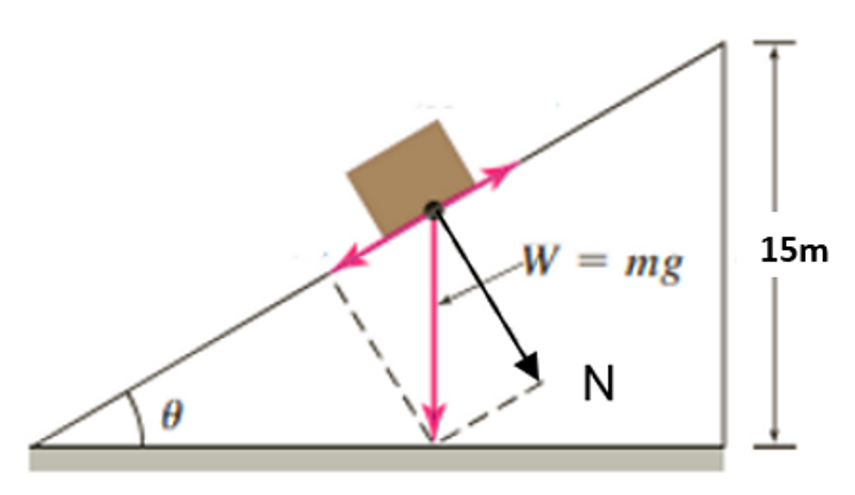
\includegraphics[scale=0.6]{Images/nocaption.png}
%	\caption[Vị trí của đá được đo từ mặt đất, xem \[4\].
%	]{\itshape\fontsize{12pt}{0pt}\selectfont\centering Vị trí của đá được đo từ mặt đất, xem \cite{ref4}.}
%	\label{hinh2.19}
\end{figure}   
\noindent a) Với $\theta ={{30}^{o}}$\\
\textbf{Trường hợp 1.}  Khi không có ma sát trượt và không có lực cản không khí.\\
Áp dụng công thức (\ref{eq:2.20}) với $v(0)=0$, do đó công thức tính vận tốc tức thời là 
$$v(t)=t\times g\times \sin \theta =t\times g\times \sin {{30}^{o}}=t\times \dfrac{g}{2}$$
Áp dụng $s'(t)=v(t)$, $s(0)=0$, ta có $s(t)={{t}^{2}}\times \dfrac{g}{4}$, chiều dài mặt phẳng nghiêng chính là quãng đường đi được của hộp, khi đó $s(t)=\dfrac{15}{\sin \theta }=\dfrac{15}{\sin {{30}^{0}}}=30\,(m)$.\\
Từ đó ta có ${{t}^{2}}\times\dfrac{g}{4}=30$ hay $t=3.5\,(s)$.\\
Vậy thời gian để hộp trượt từ đỉnh xuống chân mặt phẳng nghiêng là $3.5$ giây.\\
\textbf{Trường hợp 2.} Khi có ma sát trượt và không có lực cản không khí.\\
Áp dụng công thức (\ref{eq:2.21}) do $v(0)=0$ nên $v(t)=t[g\sin \theta -\mu gcos\theta ]$.   \\
Áp dụng $s'(t)=v(t)$, $s(0)=0$, ta có phương trình sau
$$\begin{array}{l}
s(t)=\dfrac{1}{2}{{t}^{2}}\times [g\sin \theta -\mu gcos\theta ]\\=\,\,\dfrac{g}{2}{{t}^{2}}[sin\,{{30}^{o}}-\dfrac{\sqrt{3}}{4}\cos {{30}^{o}}]=\dfrac{g}{16}{{t}^{2}}.\\
\end{array}$$
Thay $s(t)=30$ do đó $\dfrac{g}{16}\times{{t}^{2}}=30$ ta tính được $ t=7$.\\
Vậy thời gian để hộp trượt từ đỉnh xuống chân mặt phẳng nghiêng là $7$ giây.\\
\textbf{Trường hợp 3.}  Có lực ma sát trượt và có lực cản của không khí.\\
Áp dụng phương trình (\ref{eq:2.22}) ta có $$v'(t)=g\sin \theta -\mu gcos\theta -\dfrac{kv}{m}\,\,=g\times \sin {{30}^{o}}-\dfrac{\sqrt{3}}{4}g\times \cos {{30}^{o}}-\dfrac{v}{4}=\dfrac{g}{8}-\dfrac{v}{4}.$$
Với $v(0)=0$, áp dụng công thức (\ref{eq:1.8}) giải phương trình vi phân ta được 
$$v(t)=\int\limits_{0}^{t}{{{e}^{-\int\limits_{s}^{t}{\frac{1}{4}dz}}}.\dfrac{g}{2}ds}=\dfrac{g}{2}t-\dfrac{g}{2}{{e}^{-\frac{t}{4}}}.$$
Do $s'(t)=v(t)$suy ra $s(t)=\dfrac{g}{2}t+2g{{e}^{-\frac{t}{4}}}+C$. \\
Vì $s(0)=0 $ hay $2g+C=0$, do đó $C=-2g$. Vậy $s(t)=\dfrac{g}{2}t+2g{{e}^{-\frac{t}{4}}}-2g$.\\
Thay s(t)=30, giải phương trình $\dfrac{g}{2}t+2g{{e}^{-\dfrac{t}{4}}}-2g=30$ ta được $t\approx 9.8\,.$ \\
Vậy thời gian để hộp trượt từ đỉnh xuống chân mặt phẳng nghiêng là 9.8 giây.\\
b) Khi có ma sát $\left( \mu \ne 0 \right)$  nhưng không có lực cản của không khí.\\
Phương trình vi phân của mô hình là (\ref{eq:2.21}) có dạng
$$\begin{array}{l}
v'(t)=g\sin \theta -\mu gcos\theta \\ \Leftrightarrow v'(t)=g\cos \theta (\dfrac{\sin \theta }{cos\theta }-\mu )\\ \Leftrightarrow v'(t)=g\cos \theta (tan\theta -\mu ).
\end{array}$$
\textbf{Trường hợp 1.}  Nếu $\tan \theta =\mu \Rightarrow v'(t)=0\Rightarrow v(t)=C.$ \\
Mà   $v(0)=0$ nên C=0. Vậy v(t)=0, nghĩa là hộp không chuyển động.\\
\textbf{Trường hợp 2. } Nếu  $\tan \theta <\mu ;\,\,v(0)=0\,\Rightarrow v(t)=g\cos \theta (tan\theta -\mu )t<0\,\,\forall t$. \\
Vậy nếu $\tan \theta \le \mu $ thì vật không trượt xuống.\\
c) Từ phương trình vi phân (\ref{eq:2.21}) ta có
$$\begin{array}{l}
	 \,\,\,\,\,v'(t)=g\sin \theta -\mu gcos\theta \Leftrightarrow v'(t)=g\cos \theta (\dfrac{\sin \theta }{cos\theta }-\mu ) \\ 
	 \,\,\,\,\,\Leftrightarrow v'(t)=g\cos \theta (tan\theta -\mu )\Rightarrow v(t)=g\cos \theta (tan\theta -\mu )t+C. \\ 
\end{array}$$
Do $v(0)=0.3$ (m/s) ta tính được $C=0$, $\tan \theta =tan{{23}^{o}}=0.4245,\,\,\cos 23{{\,}^{o}}=~0.92,$\\
 $
 \begin{array}{ll}
 \mu ={}^{\sqrt{3}}/{}_{4}=0.4330$, $v(t)&=9.8\times 0.92.(0.4245-0.4330)\times t+0.3\\
 &=-0.077\times t+0.3
 \end{array}
 $ \\
Khi hộp dừng lại $v(t)=-0.077t+0.3=0\Rightarrow t=3.896\,(s)$. \\
Mà $s'(t)=v(t),\,\,s(0)=0$ do đó $s(t)=-0.0385{{t}^{2}}+0.3t.$\\
Độ dài mà hộp trượt đi được là $s\,(3.896)=0.548\,(m)$. \\
d) Với ${{v}_{0}}>0$ ta có $v(t)=-0.077t+{{v}_{0}}$ và $s(t)=-0.0385{{t}^{2}}+{{v}_{0}}t$ (do $s(0)=0$).\\
Quãng đường hộp trượt cần di chuyển là $s(t)=30\,(m)$, ta có phương trình
$$-0.0385{{t}^{2}}+{{v}_{0}}t-30=0.$$
Phương trình này có nghiệm khi và chỉ khi
$$\Delta \ge 0\Leftrightarrow {{({{v}_{0}})}^{2}}-4\times (0.0385)\times 30\ge 0\Leftrightarrow {{({{v}_{0}})}^{2}}\ge 4.62\Leftrightarrow \left[ \begin{array}{l}
	 {{v}_{0}}\ge 2.15 \\ 
	 {{v}_{0}}\le -2.15 \\ 
\end{array} \right.$$
Do ${{v}_{0}}>0$ nên vận tốc ban đầu nhỏ nhất là $v{}_{0}=2.15\,\,(m/s)$. \\
Khi đó $\Delta =0$ phương trình $-0.0385{{t}^{2}}+{{v}_{0}}t-30=0$ có nghiệm là $t =28$ (s).\\
Vậy thời gian hộp trượt xuống chân mặt phẳng là $28$ giây. 
\subsubsection{Mô phỏng bằng Excel}
\noindent Xét hộp trượt (trong Bài 2.9.1) trên mặt phẳng nghiêng có góc nghiêng của mặt phẳng là $\theta ={{30}^{o}}$, hệ số của ma sát trượt là $\mu =\dfrac{\sqrt{3}}{4}$ và hệ số lực cản không khí là $k=\dfrac{m}{4}$. Mô hình cho chuyển động này là
$$\begin{array}{ll}
	 v'(t)&=g\sin \theta -\mu gcos\theta -\dfrac{kv}{m}\,\,\,\\&=g\sin {{30}^{o}}-\dfrac{\sqrt{3}}{4}g\cos {{30}^{o}}-\dfrac{v}{4}\, \\ 
 &=\dfrac{g}{2}-\dfrac{3g}{8}-\dfrac{v}{4}=1.225-\dfrac{v}{4}.
\end{array}$$
Công thức tính vận tốc của hộp trượt là $v(t)=4.9-4.9{{e}^{-0.25t}}.$\\
Sử dụng tính gần đúng bằng phương pháp Euler tiến với ${{t}_{n}}={{t}_{0}}+nh$, $h=1$, và áp dụng công thức (\ref{eq:1.10})  ${{v}_{n+1}}\approx \left( 1-\dfrac{h}{4} \right){{v}_{n}}+1.225h$, ta có bảng số liệu sau (ta chỉ trích xuất các giá trị tương ứng với các số thứ tự $n$ chia hết cho $5$).
\begin{table}[H]
	\centering
	\begin{tabularx}{\textwidth}{
			|>{\centering\arraybackslash}s
			|>{\centering\arraybackslash}s
			|>{\centering\arraybackslash}y
			|>{\centering\arraybackslash}y
			|>{\centering\arraybackslash}y
			|>{\centering\arraybackslash}y|
		}
		\hline
		\bfseries  n
		&\bfseries  $\mathbf{t}_{\mathbf{n}}$
		& \bfseries Nghiệm xấp xỉ
		& \bfseries Nghiệm chính xác
		& \bfseries Sai số 
		tuyệt đối
		& \bfseries Sai số 
		tương đối (\%)
		\\
		\hline
		0  & 0  & 0           & 0           & 0           & 0           \\ \hline
		5  & 5  & 3.737207031 & 3.496126495 & 0.241080536 & 6.89564683  \\ \hline
		10 & 10 & 4.624063778 & 4.497783507 & 0.126280271 & 2.807611149 \\ \hline
		15 & 15 & 4.834519041 & 4.784763045 & 0.049755996 & 1.039884217 \\ \hline
		20 & 20 & 4.884461061 & 4.86698406  & 0.017477002 & 0.359093056 \\ \hline
		25 & 25 & 4.896312537 & 4.890540775 & 0.005771762 & 0.118018898 \\ \hline
		30 & 30 & 4.899124948 & 4.897289887 & 0.001835061 & 0.037470953 \\ \hline
		35 & 35 & 4.899792346 & 4.89922354  & 0.000568806 & 0.011610136 \\ \hline
		40 & 40 & 4.899950723 & 4.89977754  & 0.000173182 & 0.003534495 \\ \hline
	\end{tabularx}
	\caption[Bảng số liệu trong mô hình hộp trượt trong Bài 2.9.1.]{\itshape\fontsize{13pt}{0pt}\selectfont Bảng số liệu trong mô hình hộp trượt trong Bài 2.9.1.}
	\label{bang11}
\end{table}
\begin{figure}[H]
	\centering
	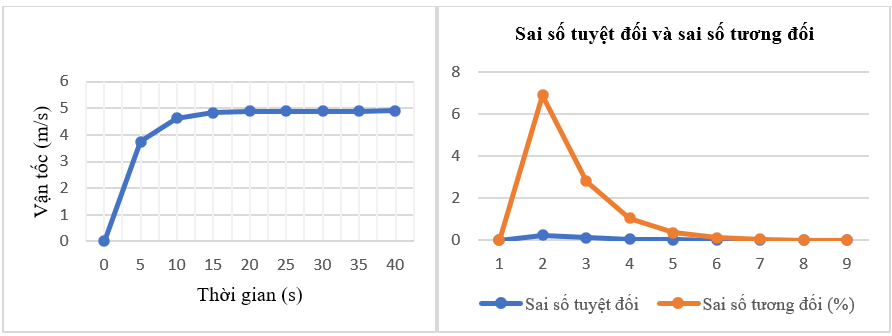
\includegraphics[scale=0.83]{Images/hinh_2_27.png}
	\caption[Biểu đồ vận tốc của hộp trượt khi có ma sát trượt và có sức cản của không khí và biểu đồ sai số trong Bài 2.9.1 tính bằng phương pháp Euler tiến.
	]{\itshape\fontsize{13pt}{0pt}\selectfont\centering Biểu đồ vận tốc của hộp trượt khi có ma sát trượt và có sức cản của không khí và biểu đồ sai số trong Bài 2.9.1 tính bằng phương pháp Euler tiến.}
	\label{hinh2.27}
\end{figure} 
\noindent\ Nhận xét: Nhìn vào bảng số liệu và Hình \ref{hinh2.27} ta thấy vận tốc tên lửa tại $t=10$s và $t=20$s xấp xỉ $4.624$ (m/s) và $4.884$ (m/s), kết quả này phù hợp với kết quả lý thuyết tính được trong Bài tập 2.9.1.
\newpage
\section*{KẾT LUẬN}
\phantomsection\addcontentsline{toc}{section}{\numberline {}KẾT LUẬN}
Luận văn tập trung phân tích và mô phỏng một số bài toán thực tế bằng phương trình vi phân tuyến tính bậc nhất như mô hình sự phát triển của vi khuẩn, sự phân hủy của chất phóng xạ, tuổi của hóa thạch, sự nóng lên/nguội đi của vật, hỗn hợp 2 dung dịch, vật rơi trong không khí, mạch điện mắc nối tiếp, chuyển động của tên lửa, hộp trượt xuống chân mặt phẳng nghiêng. 

Trong mỗi bài toán thực tế, bên cạnh việc xây dựng mô hình dưới dạng bài toán giá trị ban đầu (IVP) và tìm công thức nghiệm của các bài toán đó, luận văn còn đưa ra một số bài tập luyện tập để vừa rèn luyện cho học sinh khả năng tư duy và tính toán, cũng như hiểu rõ thêm về mô hình. Dựa vào phương pháp Euler tiến luận văn cũng sử dụng công cụ Excel để lập bảng tính các nghiệm xấp xỉ với số điểm cần thiết và vẽ đồ thị minh họa. Việc sử dụng Excel khá đơn giản, và dựa vào đồ thị có thể có cái nhìn trực quan về bài toán thực tế đang tìm~hiểu.

Tuy nhiên với một số lớp phương trình vi phân đặc biệt thì có phương pháp tìm nghiệm của chúng, nhưng không phải bất kỳ phương trình vi phân nào cũng tìm được nghiệm một cách dễ dàng. Trong khoa học, kỹ thuật đôi chỉ cần đòi hỏi độ chính xác tới một mức nào đó là chấp nhận được, do vậy việc tìm nghiệm chính xác đôi khi mất thời gian và có khi không cần thiết. Vì vậy luận văn cũng trình bày một phương pháp tính nghiệm xấp xỉ đó là phương pháp Euler tiến.
\newpage
\phantomsection\addcontentsline{toc}{section}{\numberline {}TÀI LIỆU THAM KHẢO}
% \SBtitlestyle{bar}
% \SBsubtitlestyle{none}

\begin{thebibliography}{99}
%	\addcontentsline{toc}{section}{{\bf Tài liệu tham khảo}\rm }%
	
 \centerline{\textbf{Tiếng Việt}\qquad\qquad\qquad\qquad\qquad\qquad\qquad\qquad\qquad\qquad\qquad\;\;\;}	
	
	\bibitem{ref1}
	Nguyễn Thế Hoàn, Phạm Phu (2009),
	{\it Cơ sở phương trình vi phân và lý thuyết ổn định},
	NXB Giáo dục.
	
	\bibitem{ref2}
	Trần Văn Trản (2020), 
	{\it Phương pháp số thực hành. Tập 1},
	NXB Đại học Quốc gia Hà Nội.
	
	\bibitem{ref3} 
	Trần Trung, Đặng Xuân Cương, Nguyễn Văn Hồng, Nguyễn Danh Nam (2011), 
	{\it Ứng dụng công nghệ thông tin vào dạy học môn toán ở trường phổ thông},  
	NXB Giáo dục Việt Nam.
	
	\vskip .5cm
	\centerline{\textbf{Tiếng Anh}\qquad\qquad\qquad\qquad\qquad\qquad\qquad\qquad\qquad\qquad\qquad\;\;\;}	
	
	\bibitem{ref5}
	E. Joseph Billo (2007), 
	{\it Excel for Scientists and Engineers: Numerical Methods}
	(Chapter 10), Wiley.
	
	\bibitem{ref6}
	K. K. Tung (2007), 
	{\it Topics in Mathematical Modeling}
	(Chapter 10), Princeton University Press.
	
	\bibitem{ref4}
	Dennis G. Zill (2018),
	{\it A First Course in Differential Equations with \newline Modeling Applications}
	(Chapters 1 \& 3), 11 ed., Cengage Learning.
	
	\bibitem{ref7}	
	{\it American Chemical Society National Historic Chemical Landmarks. Discovery of Radiocarbon Dating. }
	\url{http://www.acs.org/content/acs/en/education/whatischemistry/landmarks/radiocarbon-dating.html}
	
	
\end{thebibliography}



\end{document}

